\def\bbbar{\ensuremath{\mathrm{b\bar{b}}}}
\def\ccbar{\ensuremath{\mathrm{c\bar{c}}}}
\newcommand{\PZ}{Z}
\newcommand{\ZZ}{ZZ}
\newcommand{\WW}{WW}
\newcommand{\WZ}{WZ}
\newcommand{\pp}{\Pp\Pp\xspace}
\newcommand{\Wjets}{\ensuremath{\PW+\text{jets}}\xspace}
\def\Wmnbb{\ensuremath{\mathrm{W}(\Pgm\cPgn)+\bbbar}}
\def\WmnH{\ensuremath{\mathrm{W}(\Pgm\cPgn)\mathrm{H}}}
\def\Wbb{\ensuremath{\mathrm{W+\bbbar}}}
\def\hbb{\ensuremath{\mathrm{W+h\rightarrow\bbbar}}}
\def\Wc{\ensuremath{\mathrm{W+c}}}
\def\Wmn{\ensuremath{\mathrm{W}\rightarrow \mu\nu}}
\def\Wln{\ensuremath{\mathrm{W}\rightarrow \ell\nu}}
\def\Wcc{\ensuremath{\mathrm{W+\ccbar}}}
\def\Zll{\ensuremath{\mathrm{Z\rightarrow\ell\ell}}}
\def\MT{M_\mathrm{T}}
\def\ET{$E_\mathrm{T}$}
\def\pt{p_\mathrm{T}}
\def\GeV{$\mathrm{GeV}$}
\def\TeV{$\mathrm{TeV}$}
\def\tev{$\mathrm{TeV}$}
\def\PYTHIA{$\mathtt{PYTHIA}$}
\def\POWHEG{$\mathtt{POWHEG}$}
\def\MADGRAPH{$\mathtt{MADGRAPH}$}
\def\GEANTfour{$\mathtt{GEANT4}$}
\def\TAUOLA{$\mathtt{TAUOLA}$}
\def\ptvec{$\vec{p_{T}}$}
\def\VEtmiss{$\vec{MET}$}
\def\La{\mathscr{L}}
\def\fbinv{fb^\mathrm{-1}}
\def\Pg{\mathrm{g}}
\def\Pp{\mathrm{p}}
\def\Pgt{\mathrm{\tau}}
\def\tauh{\mathrm{\tau_{h}}}
\def\Pgm{\mathrm{\mu}}
\def\Pe{\mathrm{e}}
\def\cPZ{\mathrm{Z}}
\def\PW{\mathrm{W}}
\def\pt{\mathrm{p_{T}}}
\def\cPqt{\mathrm{q}}
\def\cPaqt{\mathrm{\bar{q}}}%%%%%CHECK THIS
\def\Pg{$\mathrm{g}$}
\def\vecEtm{\overline{\slash{E_{T}}}}
\def\vecPtmu{\overline{p_{T}(\mu)}}
\def\MET{\slash{E_{T}}}
\def\ttbar{${t\bar{t}}$}
\def\vecEtm{\ensuremath{\vec{E}_\mathrm{T}^{\mathrm{miss}}}\;}
\def\MET{\ensuremath{E_\mathrm{T}^{\mathrm{miss}}}\;}
\def\vecPtmu{\ensuremath{\vec{P}_\mathrm{T}^{\mu}}\;}

\newcommand{\Lint}{\ensuremath{{\cal L}_{\mathrm{int}}}}
\newcommand{\dytt}{\ensuremath{\cPZ/\Pgg^*\to\tau^+\tau^-}}
\newcommand{\dyll}{\ensuremath{\cPZ/\Pgg^*\to \ell^+\ell^-}}
\newcommand{\stat}{\ensuremath{\,\mathrm{(stat.)\;}}}
\newcommand{\syst}{\ensuremath{\,\mathrm{(syst.)\;}}}
\newcommand{\lumi}{\ensuremath{\,\mathrm{(lum.)\;}}}
\newcommand{\theo}{\ensuremath{\,\mathrm{(theo.)}}\;}



\RequirePackage{lineno}
\documentclass[oneside, letterpaper, oldfontcommands]{memoir}
%\documentclass[oneside, letterpaper, 12pt, oldfontcommands]{article}


%%%% Import uwthesis.sty to get official formatting, then set your variables.
%\usepackage{uwthesis}
%% Set the upper and lower margins (automatically adjust the textblock)
%% Upper margin needs to be larger than 1in to allow room for the page number
\setulmarginsandblock{1.5in}{1in}{*}
%% Left margin is a little larger to allow room for binding
%% Set the left and right margins (automatically adjust the textblock)
\setlrmarginsandblock{1.5in}{1in}{*}
%% Set the distance between the top of the page and the top of the header
%% The first argument is headdrop (distance from top of page to top of header)
\setheaderspaces{1in}{*}{*}
%% Implement the above changes
\checkandfixthelayout



%%%%%%%%%%%%%%%%%%%%%%%%%%%%%%%%%%%%%%%%%%%%%%%%%%%%%%%%%%%%%%%%%%%%%%%%%%%%%
%%%% INTERFACE (variables for the user to set)
%%%%%%%%%%%%%%%%%%%%%%%%%%%%%%%%%%%%%%%%%%%%%%%%%%%%%%%%%%%%%%%%%%%%%%%%%%%%%

%% For the title/committee page
\newcommand{\settitle}[1]{\def\uwtitle{#1}}  % your title
\newcommand{\setauthor}[1]{\def\uwauthor{#1}} % you
\newcommand{\setdepartment}[1]{\def\uwdepartment{#1}}  % your title
\newcommand{\masters}{\def\uwdegree{Master of Arts}}
\newcommand{\doctors}{\def\uwdegree{Doctor of Philosophy}}
\newcommand{\setgraddate}[1]{\def\uwgraddate{#1}} % graduation date
\newcommand{\setdefensedate}[1]{\def\uwdefensedate{#1}} % defense date
\newcommand{\setabstract}[1]{\def\uwabstract{#1}} % abstract

%% Members of the Final Oral Committee
\newcommand{\setfoca}[3]{\def\uwfoca{#1}\def\uwranka{#2}\def\uwdepa{#3}}
\newcommand{\setfocb}[3]{\def\uwfocb{#1}\def\uwrankb{#2}\def\uwdepb{#3}}
\newcommand{\setfocc}[3]{\def\uwfocc{#1}\def\uwrankc{#2}\def\uwdepc{#3}}
\newcommand{\setfocd}[3]{\def\uwfocd{#1}\def\uwrankd{#2}\def\uwdepd{#3}}
\newcommand{\setfoce}[3]{\def\uwfoce{#1}\def\uwranke{#2}\def\uwdepe{#3}}
\newcommand{\setfocf}[3]{\def\uwfocf{#1}\def\uwrankf{#2}\def\uwdepf{#3}}



%%%%%%%%%%%%%%%%%%%%%%%%%%%%%%%%%%%%%%%%%%%%%%%%%%%%%%%%%%%%%%%%%%%%%%%%%%%%%
%%%% REFERENCES
%%%%%%%%%%%%%%%%%%%%%%%%%%%%%%%%%%%%%%%%%%%%%%%%%%%%%%%%%%%%%%%%%%%%%%%%%%%%%
%% Make the reference section single-spaced
\let\oldbib\bibliography
\renewcommand*{\bibliography}{\SingleSpace\oldbib}
\setlength{\bibitemsep}{\onelineskip}



%%%%%%%%%%%%%%%%%%%%%%%%%%%%%%%%%%%%%%%%%%%%%%%%%%%%%%%%%%%%%%%%%%%%%%%%%%%%%
%%%% TITLE/COMMITTEE page
%%%%%%%%%%%%%%%%%%%%%%%%%%%%%%%%%%%%%%%%%%%%%%%%%%%%%%%%%%%%%%%%%%%%%%%%%%%%%

%% Command to determine how the members of the committee are formatted
\newcommand{\boxfoc}[3]{\makebox[0.4\textwidth][r]{#1} $\cdot$ \makebox[0.4\textwidth][l]{#2 of #3}}

%% Command to create the title page
\newcommand{\thetitlepage}{%
  \thispagestyle{empty}
  \begin{center}
    \vfill
    {\Large\sc\uwtitle\par}
    \vfill
    \emph{by} \\ 
    \uwauthor \\
    \vfill
    A dissertation submitted in partial fulfillment of \\
    the requirements for the degree of \\
    \vfill
    \uwdegree \\
    (\uwdepartment) \\
    \vfill
    \emph{at the} \\
    \textsc{University of Wisconsin -- Madison}\\
    \uwgraddate \\
    \vfill
    \noindent Defended on \uwdefensedate{}\\ Dissertation approved by the following members of the Final Oral Committee: \\
    \ifx\uwfoca\undefined {} 
      \else \boxfoc{\uwfoca}{\uwranka}{\uwdepa} \\
    \fi
    \ifx\uwfocb\undefined {} 
      \else \boxfoc{\uwfocb}{\uwrankb}{\uwdepb} \\
    \fi
    \ifx\uwfocc\undefined {} 
      \else \boxfoc{\uwfocc}{\uwrankc}{\uwdepc} \\
    \fi
    \ifx\uwfocd\undefined {} 
      \else \boxfoc{\uwfocd}{\uwrankd}{\uwdepd} \\
    \fi
    \ifx\uwfoce\undefined {} 
      \else \boxfoc{\uwfoce}{\uwranke}{\uwdepe} \\
    \fi
    \ifx\uwfocf\undefined {} 
      \else \boxfoc{\uwfocf}{\uwrankf}{\uwdepf} \\
    \fi
    \vfill
  \end{center}
  \clearpage
}

%%%%%%%%%%%%%%%%%%%%%%%%%%%%%%%%%%%%%%%%%%%%%%%%%%%%%%%%%%%%%%%%%%%%%%%%%%%%%
%%%% COPYRIGHT Page
%%%%%%%%%%%%%%%%%%%%%%%%%%%%%%%%%%%%%%%%%%%%%%%%%%%%%%%%%%%%%%%%%%%%%%%%%%%%%

% If you're registering copyright
\newcommand{\thecopyrightpage}{%
  \thispagestyle{empty}
  \begin{center}
    \null
    \vfill
    \copyright{} Copyright \uwauthor{} \uwgraddate{}\\
    All Rights Reserved
    \vspace{1in}
  \end{center}
}

% If you don't want to pay the copyright fee
\newcommand{\theblankcopyrightpage}{%
  \thispagestyle{empty}
  \null
  \vfill
}


%%%%%%%%%%%%%%%%%%%%%%%%%%%%%%%%%%%%%%%%%%%%%%%%%%%%%%%%%%%%%%%%%%%%%%%%%%%%%
%%%% UMI ABSTRACT
%%%%%%%%%%%%%%%%%%%%%%%%%%%%%%%%%%%%%%%%%%%%%%%%%%%%%%%%%%%%%%%%%%%%%%%%%%%%%

\newcommand{\theumiabstract}{%
  \clearpage

  %% The UMI abstract is not part of the document, so we skip pagination
  \savepagenumber
  \thispagestyle{empty}

  \begin{center}
    {\Large \textsc{\uwtitle}} \\
    \uwauthor \\
    Under the supervision of  \uwranka \uwfoca \\
    At the University of Wisconsin--Madison \\
  \end{center}

  \vspace{\baselineskip}

  \uwabstract

  \clearpage
  \restorepagenumber
}



%%%%%%%%%%%%%%%%%%%%%%%%%%%%%%%%%%%%%%%%%%%%%%%%%%%%%%%%%%%%%%%%%%%%%%%%%%%%%
%%%% Other STYLE stuff
%%%%%%%%%%%%%%%%%%%%%%%%%%%%%%%%%%%%%%%%%%%%%%%%%%%%%%%%%%%%%%%%%%%%%%%%%%%%%

% myheadings is used to define custom content for the headings
% We set headings on both odd and even pages blank, as required by UW
\pagestyle{myheadings}
\markboth{}{}

% By default, the first page of a chapter has a special style, 
% so we need to explicitly set the chapter style to myheadings as well
\aliaspagestyle{chapter}{myheadings}

% Set memoir's DoubleSpacing
\DoubleSpacing
\usepackage{graphicx}
\usepackage{mathtools}
\usepackage{subcaption}
\usepackage{graphicx}
\usepackage{caption}
\usepackage{subcaption}
\usepackage{amsfonts}
\usepackage{mathrsfs}
\usepackage{amsmath}
\usepackage{adjustbox}
\usepackage{xr}
\usepackage{multirow}
\usepackage{mathtools}
\usepackage{rotating}
\DeclarePairedDelimiter{\abs}{\lvert}{\rvert}

%\usepackage[sorting=none]{biblatex}

\settitle{A Search for Lepton Flavor Violating Decays of the Higgs Boson and a Measurement of W Boson Production using the CMS Detector at the LHC}
\setauthor{Aaron Levine}
\setdepartment{Physics}
\doctors % or \masters
\setgraddate{2016}
\setdefensedate{} % or whatever format you want

%%%% Members of the Final Oral Committee (FOC)
%%%% Give name, rank, and department
%%%% 
\setfoca{ Sridhara Dasu}{Professor}{Physics} % <- Your advisor
\setfocb{Wesley Smith}{Professor}{Physics}
\setfocc{Matt Herndon}{Professor}{Physics}
\setfocd{Lisa Everett}{Professor}{Physics}
\setfoce{Jay Gallager}{Professor}{Astronomy}

%The places you're going to are never on the map.
%-Jim Hensen

%%%% Your abstract, used for the UMI abstract and in your front matter
\setabstract{
This thesis presents the first direct search for lepton flavor violating decays of the recently discovered Higgs boson. The search is performed in the $H \rightarrow \mu \tau_{e}$ and $H \rightarrow \mu \tau_{h}$ decay channels, where $\tau_{e}$ and $\tau_{h}$ denote the electronic and hadronic tau decay channels respectively. The search is performed using the proton-proton collisions data gathered at the Compact Muon Solenoid detector at the Large Hadron Collider. The search uses 19.7 fb$^{-1}$ of $\sqrt{s}$ = 8 TeV data taken in 2012 as well as 2.3 fb$^{-1}$ of $\sqrt{s}$ = 13 TeV data taken in 2015. The limits on the branching fraction $B(H\rightarrow \mu\tau)$ are measured, and the existing limits from indirect searches are reduced by an order of magnitude. This thesis also presents a measurement of the differential cross section of a W boson produced in associated with jets. This measurement was performed with 2.5 fb$^{-1}$ of $\sqrt{s}$ = 13 TeV proton-proton collision data produced by the Large Hadron Collider in 2015 and recorded at the Compact Muon Solenoid detector. Cross sections are computed as a function of jet multiplicity, and the results are compared to theoretical predictions from leading order and next-to-leading order Monte Carlo generators.

}

%%%%%%%%%%%%%%%%%%%%%%%%%%%%%%%%%%%%%%%%%%%%%%%%%%%%%%%%%%%%%%%%%%%%%%%%%%%%%
%%%% Document
%%%%%%%%%%%%%%%%%%%%%%%%%%%%%%%%%%%%%%%%%%%%%%%%%%%%%%%%%%%%%%%%%%%%%%%%%%%%%

\begin{document}
%%%%%%SETLINE NUMBERS
%%\setpagewiselinenumbers
%\modulolinenumbers[1]
%\linenumbers
%%%%%%%END SETLINE NUMBERS
%% Tell the memoir class to set up lowercase roman for pagination, etc.
\frontmatter

%%%% Uncomment this to create a UMI abstract page.
%%%% If you are submitting electronically, however, this page is unnecessary.
 %\theumiabstract

% The title page
\thetitlepage

\title{A Search for Lepton Flavor Violating Decays of the Higgs Boson and a Measurement of W Boson Production using the CMS Detector at the LHC}
\author{Aaron Levine\\ Department of Physics\\University of Wisconsin-Madison}
\date{}
%\maketitle
% The copyright page, if you want to pay the fee and register copyright.
\thecopyrightpage
\cleardoublepage

% These above pages should not be counted, so we reset the counter to 1.
\setcounter{page}{1}

% An abstract may be required by your department.
\section{Abstract}
\uwabstract
\cleardoublepage



% Acknowledgements go here if you want to include them.
\section{Acknowledgements}
Placeholder for better acknowledgements section later. Thank parents, advisors, good teachers, fellow grad students/researchers.
\clearpage

% Table of contents

\maxtocdepth{paragraph}
\tableofcontents* % the * means that there isn't an entry for the TOC itself
\setcounter{tocdepth}{5}
\setcounter{secnumdepth}{5}
\setsecnumdepth{subsection}
 \clearpage


\makeatletter
     \renewcommand*\l@figure{\@dottedtocline{1}{1em}{3.2em}}
\makeatother
 \listoffigures*  % if you have any figures
 \clearpage
 \listoftables   % if you have any tables

% Tell the memoir class to set up normal pagination, etc. for the main doc
\mainmatter
\setsecnumdepth{subsubsection}
\chapter{Theoretical Motivation}\label{theory}
\qquad The goal of high energy particle physics is to use high energy densities to probe small distance scales and investigate properties of fundamental particles and the forces that govern them. This thesis describes the search for exotic decays of the recently discovered Higgs boson. The observation of exotic Higgs boson decays would signify the existence of new physics beyond the Standard Model, the most comprehensive theory of particle interactions to date. They would represent signs of a deeper theory that would significantly enhance our perception of forces and particles. This thesis also contains a measurement of the production of W bosons and associated jets of particles. This process involves key forces and particles of the Standard Model, and precise measurements of the process will improve understanding of the existing theory. These measurements take place at the Compact Muon Solenoid (CMS) detector using the Large Hadron Collider (LHC). 

\section{The Standard Model}\label{sm}

\qquad Our knowledge of particle interactions is summarized in a theory called the Standard Model. The theoretical framework of the Standard Model was developed over the course of the 20th century as more and more fundamental particles and forces were discovered and studied. The Standard Model is not without its flaws. Firstly, it contains many free parameters, such as the masses of the particles, that can only be determined from experiment. It also fails to include gravitational interactions, thus describing only three of the four fundamental forces. The ad hoc design of the Standard Model and the lack of grand unification provides a strong motivation for particle physicists to search for a more profound, comprehensive theory. The current state of particles physics takes a two pronged approach, with physicists making precision measurements of the Standard Model and searching for physics beyond the Standard Model. The goal is to measure the parameters of the Standard Model while searching for the theory's extension. This thesis contains both aspects. The W+jets production cross section measurement directly tests the Standard Model while the search for lepton flavor violating Higgs couplings tests hypotheses that extend the theory.

\subsection{Elementary Particles}\label{elemparticles}
\qquad The fundamental particles in the Standard Model are summarized in Figure \ref{fig:SMParticles} 

%**professional figure***lll
. The fundamental particles consist of fermions and bosons. The fermions are particles that have half integer spin, and the bosons have integer spin. Spin is the intrinsic quantized angular momentum of a particle. The bosons mediate the fundamental forces and provide mass. They will be discussed further in section \ref{elemforces} and section \ref{higgstheory}. The fermions consist of the quarks, leptons, and neutrinos. 

\qquad There are three generations of quarks, with two flavors in each generation. Each quark generation consists of a quark with +2/3 of an electron charge (+2/3e) and a quark with -1/3 of an electron charge (-1/3e). Quarks also have a property known as ``color." There are three possible colors for each quark: red, green, or blue. The concept of color is important for understanding the strong nuclear force, as discussed in section \ref{elemforces}. As shown in figure ~\ref{fig:SMParticles} the masses of the quarks vary significantly from one generation to the next.

\qquad Free quarks have never been observed in nature. Only color neutral combinations of quarks have been observed. For example, a red, green, or blue quark can form a stable state with a corresponding antiquark, with an anticolor of antired, antigreen, or antiblue. This state is known as a meson. The baryons consists of three quarks, one of each color. The proton (uud), and the neutron (udd), are both baryons. Matter than is composed of quarks is called hadronic matter. At CMS, hadrons are often found in collimated streams of particles known as jets. 

\begin{figure}[here]
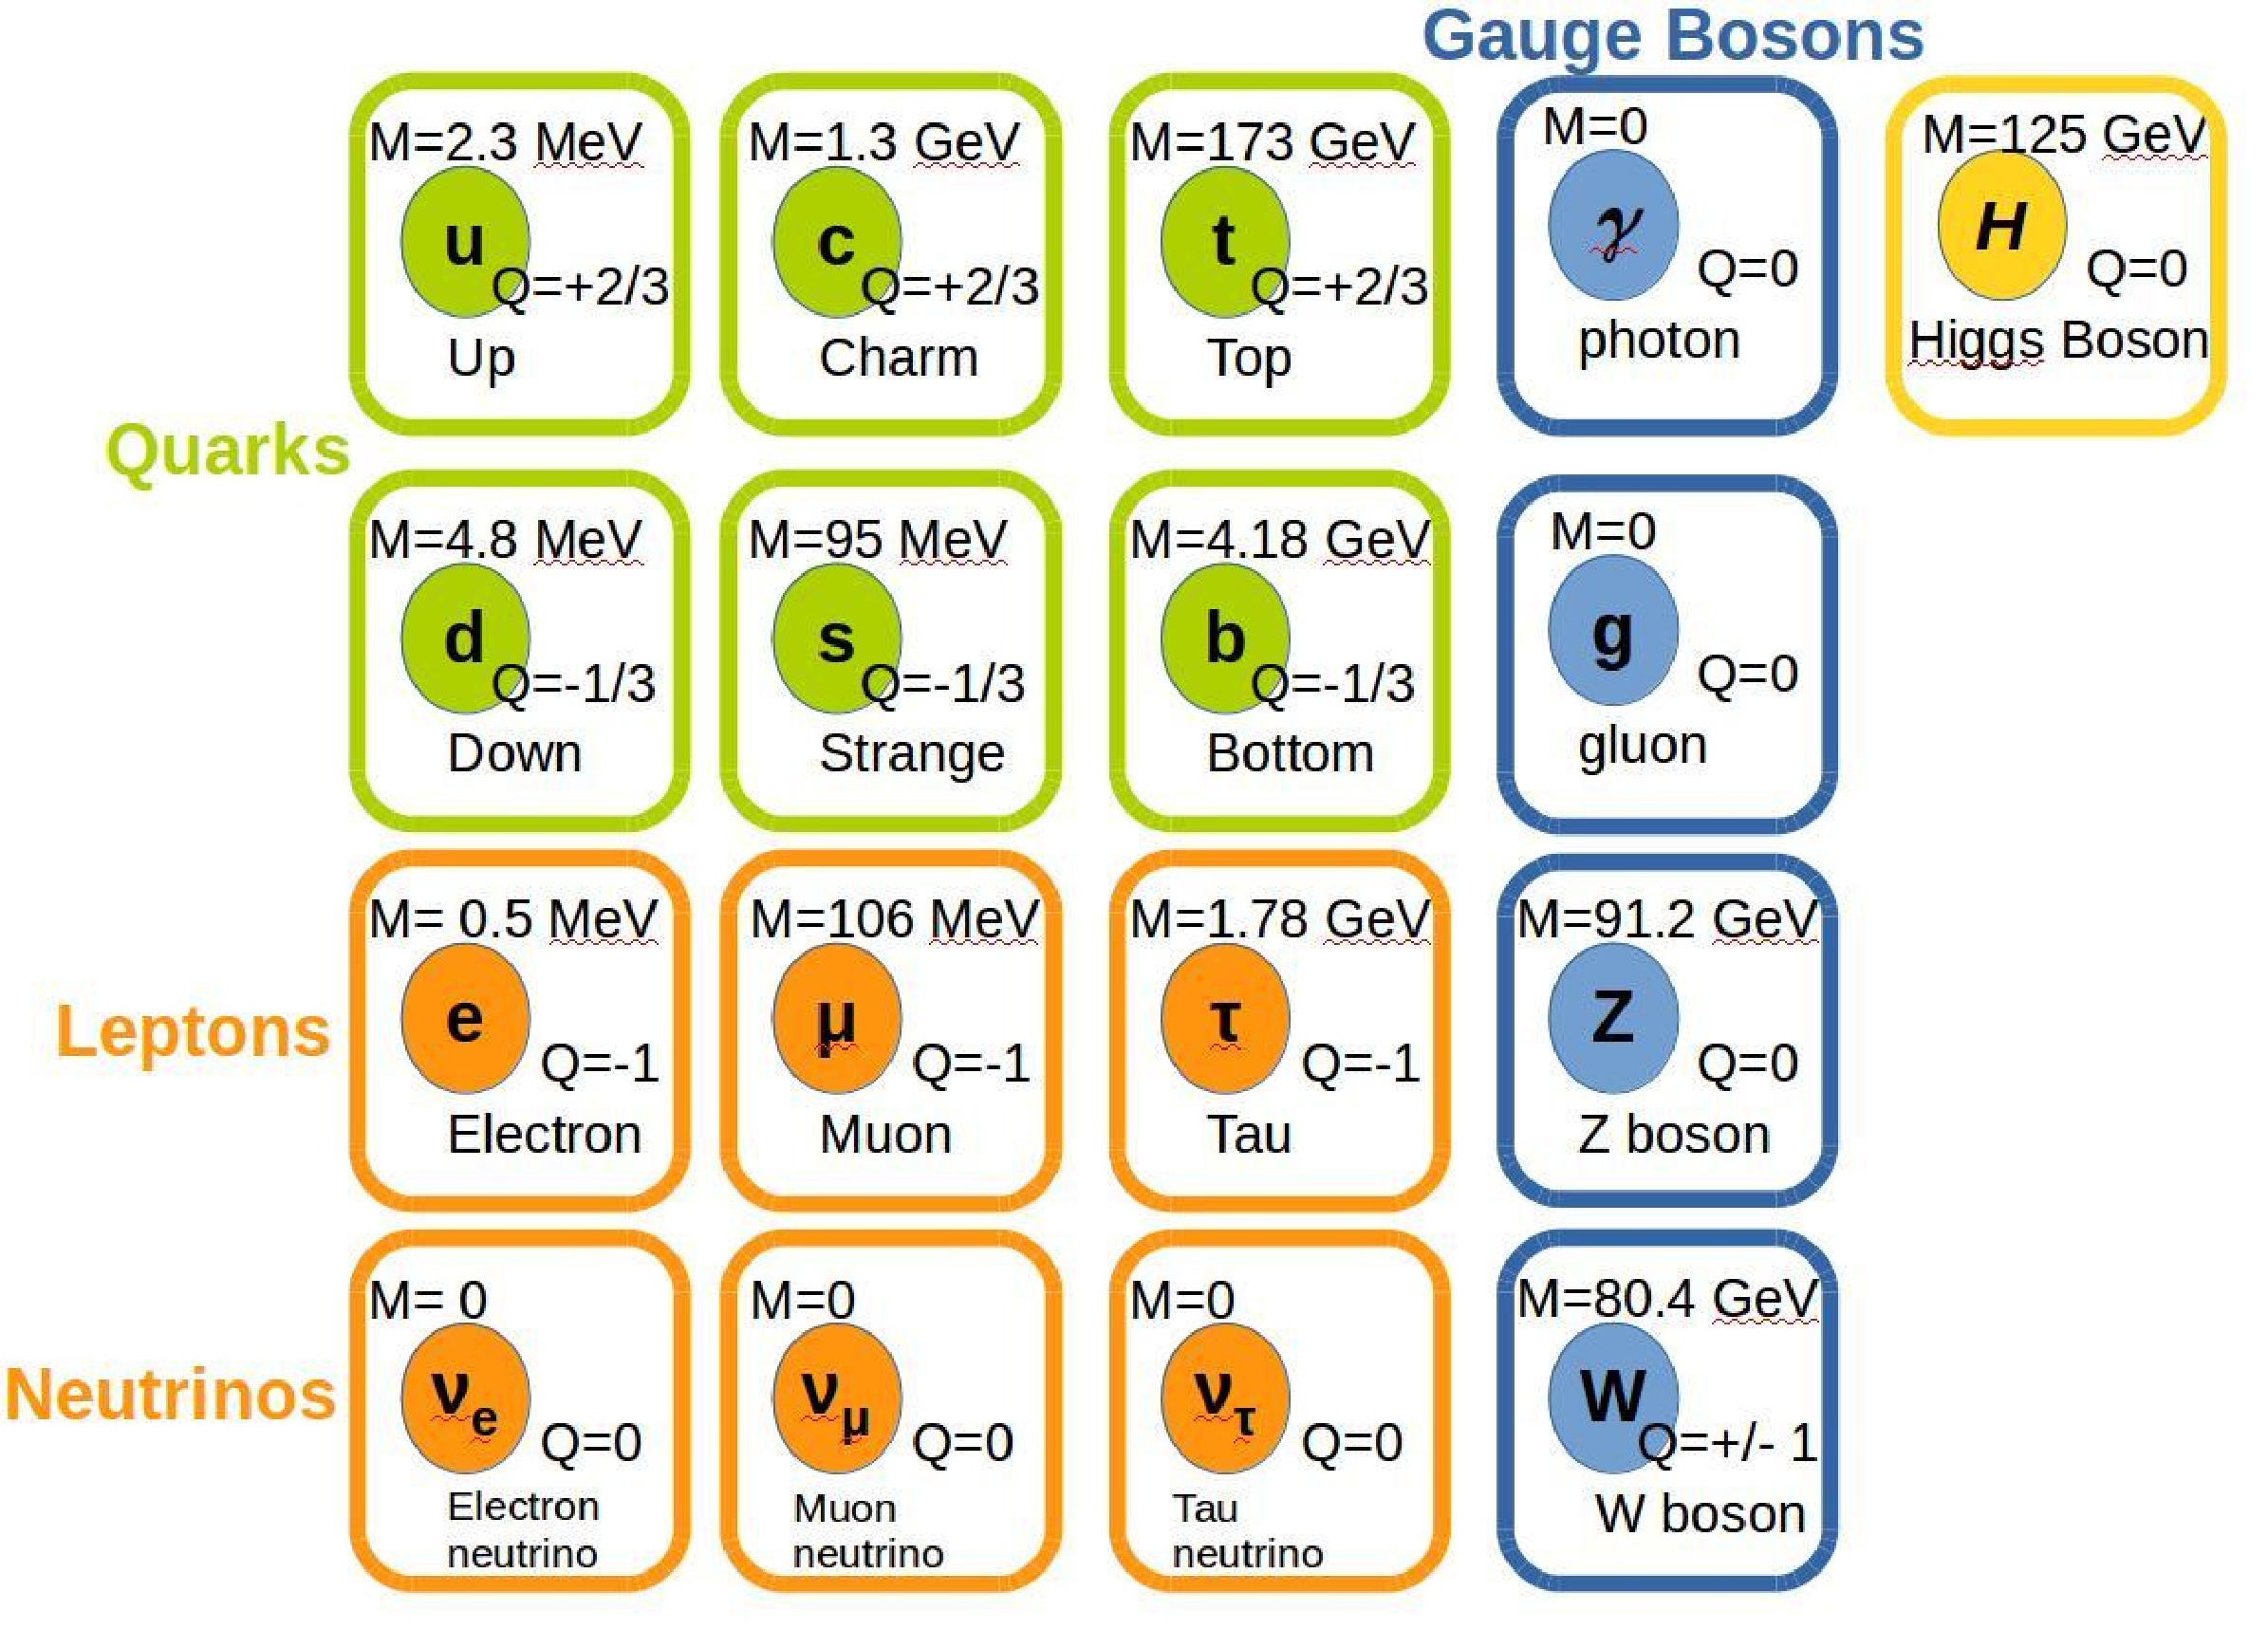
\includegraphics[width=0.9\textwidth]{StandardModel.pdf}
\caption{The fundamental particles of the Standard Model. Charges are expressed in units of electron charge.\cite{Agashe:2014kda} }
\label{fig:SMParticles}
\end{figure}


%Mesons consist of a quark antiquark pair, and baryons consist of three quarks, such as the proton (uud). In both cases, the charges of the quarks must sum to an integer multiple of the electron charge. Particles with non integer charges are not found by themselves in nature. It should be noted that it is simplistic to model a proton as a collection of two up quarks and a down quark. Those three quarks are known as valence quarks, which give the proton its charge and spin. In high energy collisions the "sea quarks," which are a vast number of quark antiquark pairs, dominate the model. This will be discussed further in chapter 2 ***. All matter that is made out of quarks is known as hadronic matter.

\qquad There are three generations of leptons, each with a neutrino pair. The electron is extremely light and does not decay, but the muon and the tau are heavier and have lifetimes on the order of $10^{-6}s$ and $10^{-15}s$ respectively\cite{Agashe:2014kda}. The mechanisms for lepton decay will be discussed in section \ref{elemforces} . In the Standard Model, there is a conserved quantity known as the lepton number. The lepton number is defined for each lepton generation. Each lepton/neutrino pair in the generation has a generation lepton number of one and the corresponding antiparticle pair has a generation lepton number of -1. For example, and $e$ and an $\nu_{e}$ each will have an electron lepton number of 1, and the corresponding antiparticle pair will have an electron lepton number of -1. Figure~\ref{fig:TauDecay} gives an example of a typical Standard Model decay that conserves lepton number. In the initial state only the tau exists and the tau lepton number of the system is one while the muon and electron lepton numbers of the system are 0. The decay produces a tau neutrino which also has a tau lepton number of one along with an electron and an antielectron neutrino, which have electron lepton numbers of one and negative one, respectively. So the final state also has a tau lepton number of one. Also note that lepton number and flavor are conserved at each vertex. In the lepton flavor violating couplings studied in this thesis, a muon and a tau share a vertex, which is not allowed in the Standard Model. 
%*** professional feynman diagrams ***

Figure \ref{fig:TauDecay} displays an example of a Feynman diagram, which are pictorial representations of particle interactions. These diagrams are actually very powerful tools in high energy physics because they used to calculate the matrix elements of the interaction. Matrix elements are used to compute the cross sections, which, as described in section \ref{elemforces}, are a measurement of the likelihood of the process occurring. Matrix elements can be thought of as an entry in the matrix $V_{if}$, which relates a particle in the initial state $i$ to the final state $f$ via a potential $V$. The square of the matrix element will define the probability of the transfer occurring.

\begin{figure}[here]
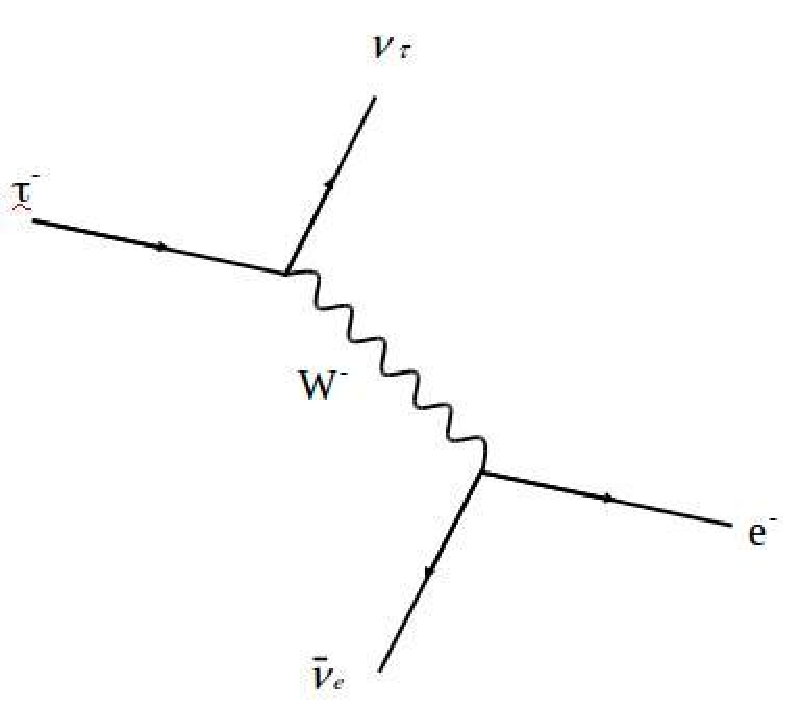
\includegraphics[width=0.4\textwidth]{TauDecay.pdf}
\caption{Decay of the tau lepton, as mediated by the W boson. The W boson is discussed further in section \ref{elemforces}.}
\label{fig:TauDecay}
\end{figure}

\subsection{Elementary Forces}\label{elemforces}

\begin{table}[htbp]
  \centering
  \begin{tabular}{ | l | c | r |}
    \hline
    Force & Relative Strength & Mediator \\ \hline \hline
    Strong & 1 & Gluon \\ \hline
    Electromagnetic & $10^{-3}$ & Photon \\ \hline
    Weak & $10 ^{-11}$ & W,Z Boson \\ \hline
    
  \end{tabular}
  \caption{Fundamental forces of the Standard Model\cite{Halzen:1984mc}.}
  \label{tab:FundForces}
\end{table}

\qquad The fundamental forces of the Standard Model are shown in Table~\ref{tab:FundForces}. Note that gravity is not included in the table. Gravity is not contained in the Standard Model and has a strength on the order of $10^{-30}$ \cite{Barger:0201058766} relative to the weak nuclear force. It plays a negligible role in high energy physics.

\qquad The theory of the electromagnetic force is known as quantum electrodynamics (QED). The electromagnetic force is mediated by the photon, which is a spin 0 massless particle and only interacts with particles that carry charge. Two examples of electromagnetic interactions are show in figure~\ref{fig:eeScattering}.

\begin{figure}[here]
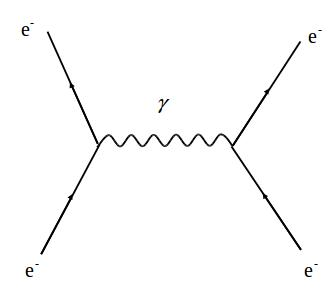
\includegraphics[width=0.4\textwidth]{eeScattering.jpg}
\caption{A photon mediating scattering between two electrons}
\label{fig:eeScattering}
\end{figure}


\qquad The weak nuclear force is mediated by the W and Z bosons. The Z boson is a massive neutral spin 1 particle. It decays into pairs of quarks, leptons, or neutrinos. The W boson is a massive charged spin 1 particle. It has the special property of changing flavors of quarks and leptons. For example, the W boson can mediate the decay of a tau to an electron. This is illustrated in figure ~\ref{fig:TauDecay}. Note that lepton number is still conserved in these types of interactions. The W boson can change flavors of leptons in accordance with the Cabbibo-Kobayashi-Maskawa (CKM) matrix\cite{Agashe:2014kda} shown in equation\ref{eq:ckm}. The CKM matrix is a unitary matrix whose elements $|V_{ij}|^{2}$ give a measure of the likelihood of a W boson mediating the transition from quark $i$ to quark $j$. As shown in equation \ref{eq:ckm}, these transitions are favored for quarks in the same generation, but are not entirely forbidden for quarks in different generations. The weak nuclear force only involves ``left handed" doublets of quarks and neutrinos. The concept of ``handedness" is defined by helicity. Right handed particles are those with parallel spin and momentum vectors, and left handed particles have anti parallel spin and momentum vectors. Only left handed particles participate in the weak interaction.

\begin{equation}
\label{eq:ckm}
\left| \begin{array}{ccc} V_{ud} & V_{us} & V_{ub} \\ V_{cd} & V_{cs} & V_{cb} \\ V_{td} & V_{ts} & V_{tb} \end{array} \right| = \left| \begin{array}{ccc} 0.97 & 0.23 & 0.004 \\ 0.23 & 0.99 & 0.04 \\ 0.009 & 0.04 & 0.999 \end{array} \right|
\end{equation}

\qquad The theory of the strong nuclear force is known as quantum chromodynamics (QCD). The strong nuclear force is mediated by the gluon. Each gluon is a color doublet, with a corresponding color and anticolor. For example, a gluon could be red and antigreen, or blue and antired, et cetera. Gluons only interact with particles that share one of their color charges. Therefore, the quarks are the only particles involved in strong interactions. Virtual gluons can self interact which increases the strength of the color charge surrounding a quark. At small distance scales the virtual gluon cloud is penetrated and the effective color charge decreases. This effect is known as asymptotic freedom. \cite{Halzen:1984mc} At larger distances, as a quark antiquark pair move apart from each other, the increase in potential energy allows new quark antiquark pairs to be created from the vacuum. The new quarks will be bound to the initial quarks by the strong nuclear force, which is why free quarks have never been observed. 
\qquad The coupling constant for QCD, $\alpha_{s}$, is energy dependent and scales as $\alpha_{s}(Q^{2}) \propto 1/ln(\frac{Q^{2}}{\Lambda_{QCD}^{2}})$. Here $Q^{2}$ represents the momentum transfer of the process and $\Lambda_{QCD}$ is a constant, referred to as the QCD scale, with a measured value of 214 MeV\cite{Agashe:2014kda}. At the TeV scale collision energies of the Large Hadron Collider, $\alpha_{s}$ is small and interactions are modelled using perturbative QCD (pQCD). Leading order terms that depend on $\alpha_{s}$ and next to leading order terms that depend on $\alpha_{s}^{2}$ dominant the computation and higher order terms can be neglected.

\qquad As mentioned in section \ref{wboson}, both the strong force and the weak force play important roles in the production of W bosons and associated jets. The strong force governs quark-gluon interactions and jet formation, while the weak force is responsible for the W boson couplings to initial start quarks and final state muons. Thus, a precision measurement of W+jets production is an powerful channel to evaluate the accuracy of the Standard Model.



\subsection{The Higgs Boson}\label{higgstheory}
\qquad In classical physics, the equations of motion of a system are governed by the Lagrangian. The Lagrangian is defined as $L = T - V$ where $T$ is the kinetic energy and $V$ is the potential energy. In the Standard Model, we can also define a Lagrangian that governs all particle interactions\cite{Halzen:1984mc} However, when mass terms for W and Z bosons are added to the Lagrangian, the Standard Model breaks down. Loops formed by W and Z bosons contribute infinities to Standard Model calculations that cannot be removed. This means that the Standard Model becomes non renormalizable. 

\begin{figure}[here]
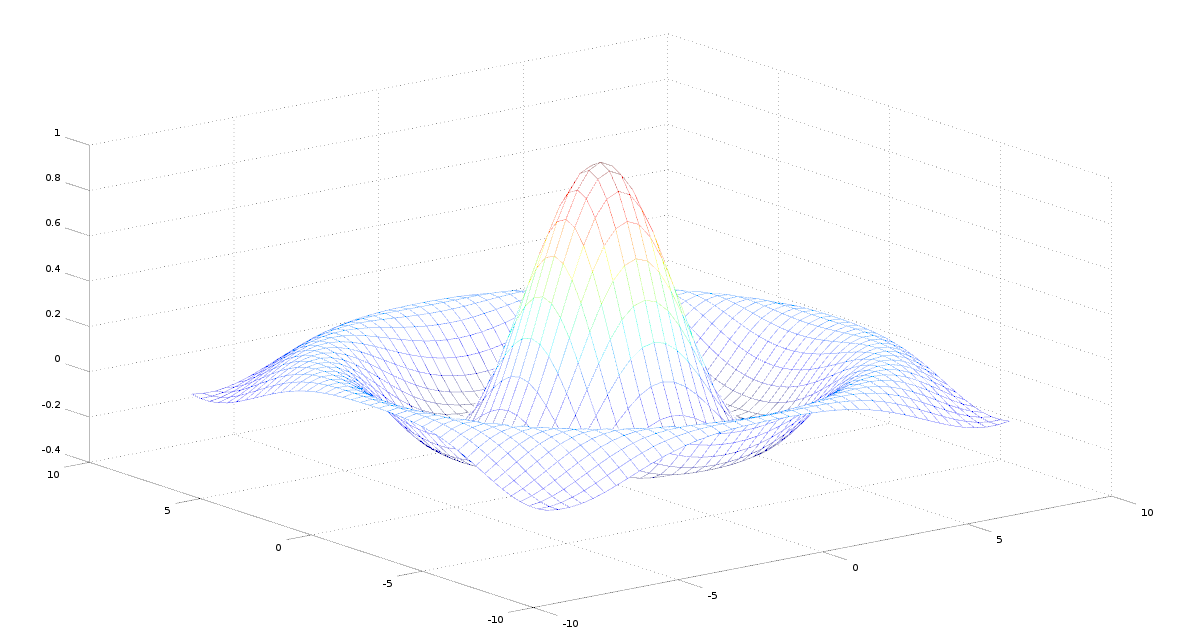
\includegraphics[width=0.9\textwidth]{HiggsPotential.png}
\caption{The potential of the Higgs Field. Note the nonzero minima.}
\label{fig:HiggsPotential}
\end{figure}

\qquad To resolve this, we introduce a field with a potential shown in figure ~\ref{fig:HiggsPotential}. This potential has a minimum that is not at the origin of the coordinate system. We can break the symmetry by shifting our reference point to the minimum of the potential and expanding for small deviations about the minimum. When this shift is introduced to the Lagrangian, it results in mass terms appearing for the W and Z bosons, the quarks and leptons, and a mass term for the particle associated with the field itself. That particle is known as the Higgs Boson. In addition to providing the theoretical framework to add mass terms to the Lagrangian, the Higgs Boson couples to every massive particle in the Standard Model. These couplings are called Yukawa couplings. The couplings of the Higgs to the W and Z bosons cancel out the infinities mentioned earlier.\cite{Halzen:1984mc} Thus, the field that naturally gives rise to masses in the Standard Model also cancels out the divergences that prevented us from simply placing mass terms in the Lagrangian to begin with. A Higgs Boson with a mass of 125 GeV was discovered at CERN on July 4 2012. \cite{Agashe:2014kda}
 

\section{Beyond the Standard Model}\label{BSM}

\qquad As mentioned in section \ref{sm} the Standard Model requires many free parameters determined by experiment and fails to unify gravity with the other four fundamental forces. Additionally, it doesn't address the hierarchy problem\cite{ArkaniHamed:1998rs}. 

Quantum field theory states that the masses of particles from scalar fields, such as the Higgs, are vulnerable to quantum corrections. The large difference in strength between the weak nuclear force and gravity (section \ref{elemforces}) means that these quantum corrections can raise the Higgs mass all the way up to the mass scale of gravity, on the order of $10^{18}$ GeV. The paradox between the existence of a low mass scalar Higgs needed for electroweak symmetry breaking and the fact that such a low mass scalar particle seems prohibited by quantum field theory is known as the hierarchy problem. The hierarchy problem can be solved by specifying a partner for each existing Standard Model particle, such that the loop corrections to the Higgs mass from the existing standard model particle and its partner cancel out, leaving the Higgs mass stable. This solution to the hierarchy problem is known as Supersymmetry. In particular, supersymmetry states that each boson has a fermion superpartner whose spin differs by $1/2$ from the boson's spin, and vice versa. This will require at least one additional Higgs doublet field\cite{Csaki:1996ks}. Supersymmetry has yet to be observed, and much is unknown experimentally about the couplings that will solve the hierarchy problem. Higgs couplings that involve heavier leptons, such as a tau, will be stronger and play a larger role in the Higgs mass than couplings to muons, electrons, and the lighter quarks. Therefore, lepton flavor violating couplings such as  $Y_{\mu\tau}$ will play a significant role in calculations related to the hierarchy problem. One can think of a matrix of $Y_{ij}$ couplings between leptons $i$ and $j$ as analogous to the CKM matrix discussed in section \ref{elemforces}.

A more fundamental theory must exist, and the recently discovered Higgs boson provides a rich environment for probing the existence of such a theory. Many proposed theories that solve the hierarchy problem, such as Randall-Sundrum models \cite{Randall:1999ee} or supersymmetric Two Higgs Doublet models \cite{Branco:2011iw} 
predict a Higgs boson with couplings that violate lepton flavor conservation. The strength of Higgs couplings are proportional to the masses of the particles involved, so the most logical place to start a search for lepton flavor violation would be a Higgs boson coupling directly to the two heaviest leptons: a muon and a tau.

\qquad There have been no direct searches for $H \rightarrow \mu\tau$ prior to the result contained in this dissertation. Null searches for $\tau \rightarrow \mu\gamma$ constrain the branching fraction for $H \rightarrow \mu\tau$ to $\mathcal{O}(10\%)$.\cite{Harnik:2012pb}

\qquad Lepton flavor violating couplings may explain a discrepancy in the anomalous magnetic moment of the muon. The magnetic moment is a quantity defined for a current loop that describes the torque the current loop experiences in a magnetic field. Muons are point particles, so according to classical electrodynamics they lack a magnetic moment. However, in QED, loop interactions will effectively generate a magnetic moment, known as the anomalous magnetic moment of the muon. The current measured value differs from the expected standard model value by $2.87 \times 10^{-9}$, a significance of $3.6 \sigma$ \cite{Bennett:2004pv}\cite{Agashe:2014kda}. Loop corrections, as shown in Figure\ref{fig:mutauloop} from a Higgs coupling to a muon and a tau could resolve this discrepancy \cite{Harnik:2012pb}. 
%***professional feynman diagrams***

\begin{figure}[here]
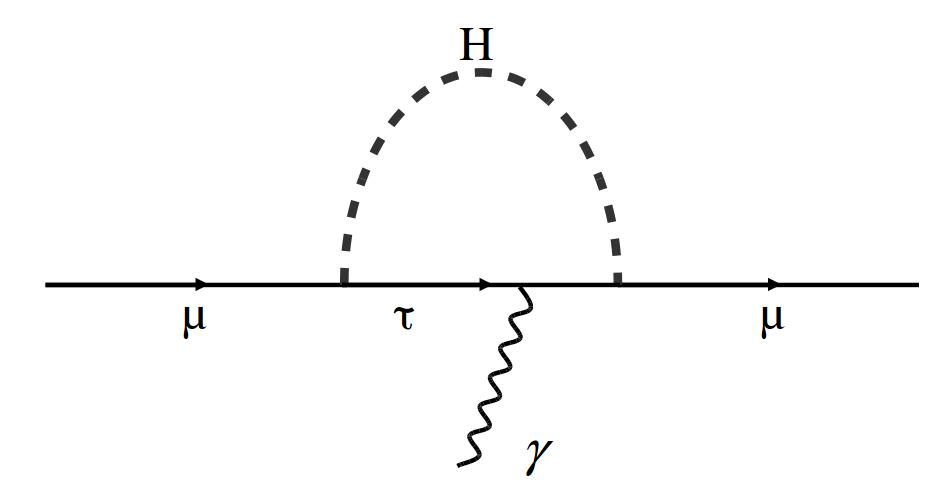
\includegraphics[width=0.9\textwidth]{mutauloop.jpg}
\caption{Loop contribution of lepton flavor violating couplings between muons and taus to the anomalous magnetic moment of the muon.}
\label{fig:mutauloop}
\end{figure}

\chapter{Collider Phenomenology}\label{pheno}
\qquad Now that the underlying physics has been described in sections \ref{sm} and \ref{BSM}, the question remains: how exactly are W+jets and lepton flavor violating Higgs events produced and studied? Before proceeding further, some basic terms of collider physics must be defined. The cross section of a particle interaction is an effective area that gives a sense of the likelihood of the interaction. In collider physics, cross sections are measured in barns (b), where $1b = 10^{-24}cm^{2}$. The luminosity is defined as the rate of observed events divided by the cross section. The integrated luminosity is computed by summing the luminosity with respect to time. Integrated luminosity is used to define how much total data has been used in a measurement. These terms will be used for describing proton proton collisions, W boson production, and Higgs boson production in the coming sections of this chapter.

\section{Kinematics Definitions}\label{kindef}
\qquad The subsequent sections in the chapter require knowledge of relevant kinematic variables, which will be defined here. The protons are accelerated up to almost the speed of light, so a relativistic treatment must be used to study the collisions.   In special relativity, the energy of the system, $E$, is defined as $E^{2} = m^{2}+p^{2}$. Here the speed of light, $c$, is set to 1, in accordance with natural units. The energy momentum 4-vector is defined as $ \hat{P} = (E, \vec{p})$, and the dot product is defined such that $\vec{P} \dot \vec{P} = E^{2}-p^{2}$, which is the Lorentz invariant mass of the particle. The square of the sum of four momentum vectors gives the invariant mass of a system of particles. Lorentz invariant quantities are useful because they are independent of the frame of reference. 

\qquad For two colliding particles, $p_{1}$ and $p_{2}$ we can define a quantity: $s = (p_{1}^2+p_{2}^2)$, which is the Lorentz invariant square of the total center of mass energy of the event. This variables is used to express the energy of particle collisions.

\qquad The rapidity $y$ of a particle is defined as: $y = \frac{1}{2}ln(\frac{E+p_{z}}{E-p_{z}}$, where $p_{z}$ is the component of the momentum parallel to the beam axis. The rapidity gap between two particles, $\Delta y_{12}$, is Lorentz invariant. The pseudorapidity $\eta$ is defined as : $\eta = \frac{1}{2}ln(\frac{p+p_{z}}{p-p_{z}}$. This can be expressed in terms of polar angle (section \ref{cms}) as $\eta = ln(cot(\theta /2))$. The pseudorapidity is equal to the rapidity if the rest mass is 0. At high energy collisions at the LHC, $E \gg m$ and $y \approx \eta$.

\section{Proton-Proton Collisions}\label{ppcoll}
\qquad The Large Hadron Collider (LHC), which will be discussed further in section \ref{lhc}, is a proton-proton collider. The proton, as mentioned in section \ref{elemparticles}, is considered to be the bound state of three quarks: two up quarks and a down quark. However, proton-proton collisions cannot simply be thought of as six up and down quarks interacting. Inside the proton, massive amounts of quark and antiquark pairs, known as ``sea quarks", pop in and out of existence, along with the gluons that bind them together. At the high energies and short distance scales probed by the LHC, the valence quarks play essentially no role in the outcome of these collisions. In fact, the gluons carry about 50$\%$ of the proton's momentum\cite{Halzen:1984mc}, and at high momentum transfer they play the dominant role in LHC collisions, as shown in Figure \ref{fig:cteq6PDF} .So when two protons collide at the LHC, it is effectively a collision between two clouds of gluons and quarks.These collisions can be studied via the parton model. This model defines the protons as collections of point particles (partons) carrying a fraction $x$ of the hadron's momentum. The distribution of $x$ depends on the momentum scale $Q^{2}$ that is probed. 

\qquad When the two proton beams in the LHC intersect, the partons from one beam will interact with the partons from the other beam. In each collision there will be multiple high momentum transfer, ``hard" scattering interactions between different pairs of protons. As discussed in section \ref{trigger}, the probability of producing an interesting physics event with high energy leptons or hadrons is low. Therefore, each time a physics event is stored for detailed analysis, in addition to the high energy, hard scattering process of interest, there will be additional hard scattering processes in the event. These additional hard scattering interactions are referred to as ``pileup". The additional particles produced threaten to cloud our knowledge of the hard scattering process at the primary vertex. Methods of vetoing and subtracting pileup contributions to the event are discussed in sections \ref{electrons}, \ref{muons}, and \ref{hadrons}. The ``underlying event" includes any particles in the event not due to the hard scattering process of interest. In addition to pileup, this includes intial and final state radiation from the beam, as well as lower energy ``soft" scattering interactions between protons. 

\qquad As quarks and gluons move apart after the collision, the increase in potential energy from the strong interaction produces a stream of collimated hadrons, known as a jet. Jet formation is shown in Figure \ref{fig:JetFormation}. First, energetic quarks radiate gluons, which split into quarks. These quarks may still be energetic enough to radiate gluons, and the process continues. This is known as parton showering. Detailed simulations of this process are described in section \ref{partonshower}. QCD confinement requires that the quarks and gluons are naturally grouped into colorless clusters. These clusters then separate into groups of hadrons after the conclusion of parton showering, which is known as hadronization. The identification of jets is discussed in section \ref{jets}. 

\begin{figure}[here]
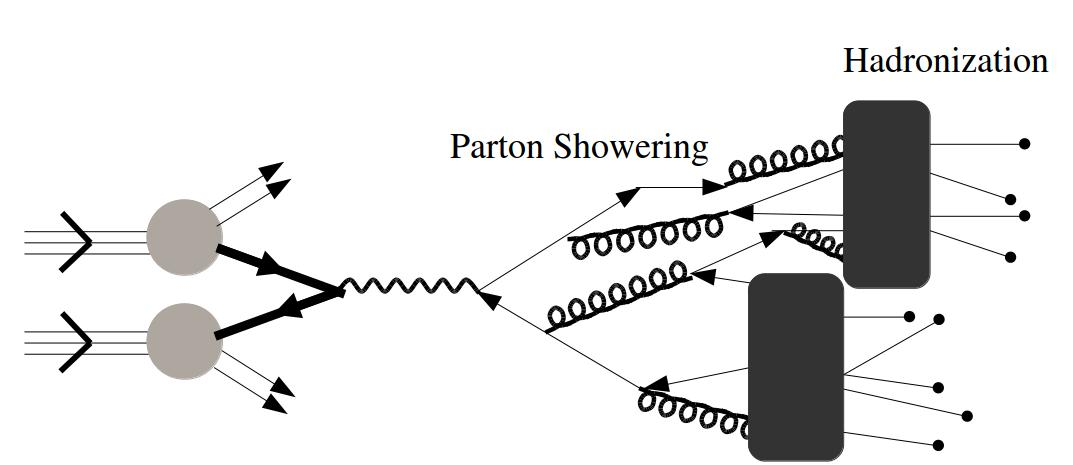
\includegraphics[width=0.9\textwidth]{jetformation.jpg}
\caption{Diagram of jet formation occurring after a hard scatter event. First quarks and gluons are radiated in parton showering. Then they combine into colorless cluster before condensing into the hadrons that make up jets.}
\label{fig:JetFormation}
\end{figure}



\section{W Boson Production}\label{wboson}
\qquad W bosons are produced by deep inelastic scattering between partons, as show in Figure \ref{fig:WFormation}. The cross section of this process depends on the parton distribution functions. Examples of CTEQ6 parton distribution functions are show in Figure \ref{fig:cteq6PDF}\cite{Pumplin:2002vw}. These parton distribution functions are used in {\sc Pythia}, as discussed in section \ref{partonshower}.

\begin{figure}[here]
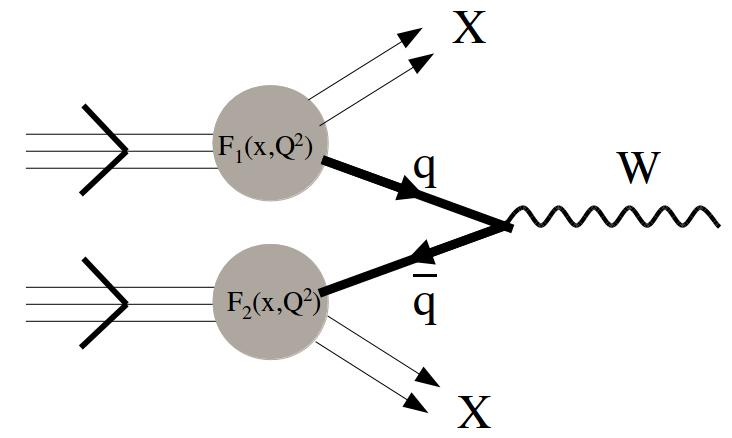
\includegraphics[width=0.9\textwidth]{WFormation.jpg}
\caption{Diagram of W Boson production. The function $F_{1}$ and $F_{2}$ are the parton distribution functions of the incoming protons.}
\label{fig:WFormation}
\end{figure}

\begin{figure}[here]
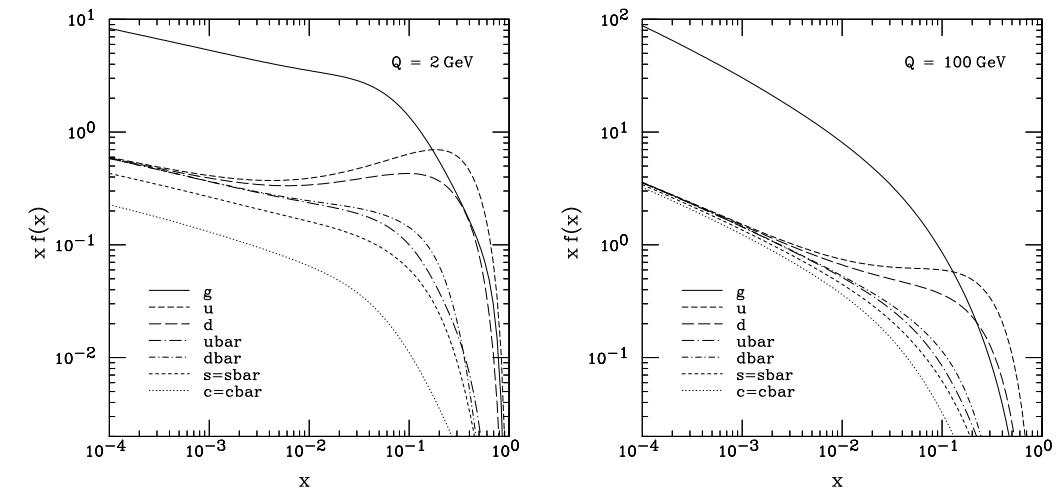
\includegraphics[width=0.9\textwidth]{cteq6PDF.jpg}
\caption{Parton distribution functions in the CTEQ6 scheme\cite{Pumplin:2002vw}. As the energy $Q$ of the collision increases, the quarks involved carry less and less of the proton's momentum and the applicability of pQCD increases.}
\label{fig:cteq6PDF}
\end{figure}

\qquad W bosons decay to leptons and quarks at equal rates. The W may decay to an up/down quark pair, a charm/strange quark pair, or a lepton/lepton neutrino pair. The presence of the associated neutrino in the final state of the leptonic decay is necessary to conserve lepton flavor in the Standard Model, as discussed in section \ref{elemforces}.  The decay to a bottom/top quark pair is suppressed because of the high mass of the top quark. Each quark has three flavors, and there are three total leptons, so ultimately W decay has six hadronic final states and three leptonic final states. This means that W bosons decay to hadrons approximately 67$\%$ of the time and decay to leptons about $33\%$ of the time. As discussed in section \ref{muonsys}, due to CMS's ability to detect and reconstruct muons with high efficiency, we look for W bosons decaying to a muon and a muon neutrino. Because of lepton universality, the branching fraction of $W \rightarrow \mu\nu_{\mu}$ is about 11$\%$. 

\qquad W boson production is studied based on the number of jets produced in association with the W boson. An example of a single radiated jet is shown in Figure \ref{fig:WOneJet}. The cross section for W boson production from two partons scattering is given by equation \ref{eq:wprod} \cite{Barger:0201058766}. Here, $V_{ud}$ defines the probability for up-down quark transitions, $G_{F}$ is a fundamental constant of the Standard Model, $M_{W}$ is the mass of the W boson, and $\hat{s}$ is the momentum of the diquark system. The hats on $\hat{s}$ and $\hat{\sigma}$ indicate that these values apply to one parton scatting off of another parton. To calculate the full cross section of W production we must integrate over the parton distribution functions of the quarks involved.

\begin{equation} \label{eq:wprod}
\hat{\sigma}(u d \rightarrow W) = 2\pi |V_{ud}|^{2}\frac{G_{F}}{\sqrt{2}}M_{W}^{2}\delta(\hat{s} - M_{W}^{2})
\end{equation}

\begin{figure}[here]
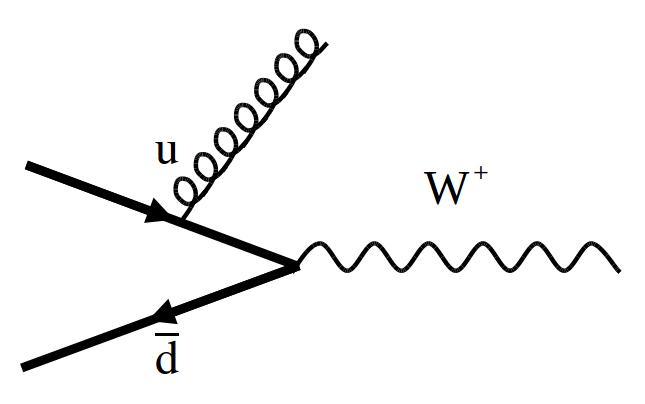
\includegraphics[width=0.7\textwidth]{WOneJet.jpg}
\caption{Example of the production of a W plus one jet event.}
\label{fig:WOneJet}
\end{figure}

Previous results from CMS measured at 7 TeV center of mass collisions\cite{Khachatryan:2014uva} are shown in Figure \ref{fig:wjets7TeV}. 

\begin{figure}[here]
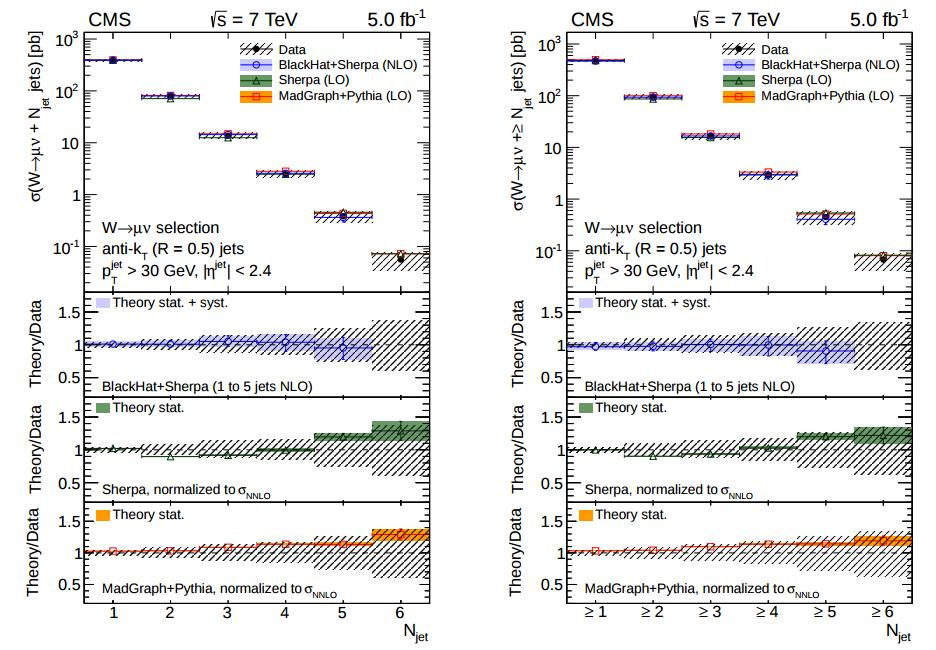
\includegraphics[width=0.9\textwidth]{wjets7TeV.jpg}
\caption{W+jets production at CMS in 2011. Cross sections are show in units of picobarns. The left plot shows exclusive jet binned (= NJets) results and the right plot shows inclusive jet binned ($\geq$ NJets) results. Comparisons between theoretical predictions and data are shown in the ratio plots. Agreement is within statistical uncertainty. }
\label{fig:wjets7TeV}
\end{figure}


\section{Higgs Boson Phenomenology}\label{higgspheno}
\qquad As mentioned in section \ref{higgstheory}, the Higgs boson couples to all massive Standard Model particles, and the couplings take the form of mass terms in the Standard Model Lagrangian. The discovery of a Higgs boson with a mass of 125 GeV was announced on July 4 2012. The Higgs was discovered by searching for its signature decays, as shown in figure \ref{fig:higgsBR}. The search was carried out in the $b\bar{b}$, WW, ZZ, $\tau\tau$, and $\gamma\gamma$ channels \cite{Khachatryan:2016vau}. The largest significances were found in the ZZ and $\gamma\gamma$ channels. Those channels only required the straightforward reconstruction of electrons, muons, and photons, whereas the WW channel required the reconstruction of missing energy (section \ref{met}), the $\tau\tau$ channel required the reconstruction of missing energy and hadronic taus (section \ref{taus}) and the $b\bar{b}$ channel required the reconstruction of b-jets (section \ref{bjets}). Note that the $H \rightarrow \gamma\gamma$ channel does not imply that the Higgs couples directly to massless particles like the photon. The Higgs boson couples to photons via quark or vector boson loops, as shown in figure \ref{fig:higgsgg}. Expected Standard Model branching ratios in the channels used to discover the Higgs are given in table \ref{tab:higgsbr}. The agreement between theory and experiment is shown in figure \ref{fig:higgsSMBR}. 

%\begin{table}[htbp]
%  \centering
%  \begin{tabular}{ | l | c | c |}
%    \hline
%    Channel & Expected ($\sigma$)  & Observed ($\sigma$) \\ \hline \hline
%     ZZ & 3.8 & 3.2 \\ \hline
%     $\gamma\gamma$ & 2.8 & 4.1 \\ \hline
%    WW & 2.5 & 1.6 \\ \hline
%    $b\bar{b}$ & 1.9 & 0.7 \\ \hline
%    $\tau\tau$ & 1.4 & - & \\ \hline
%    
%  \end{tabular}
%  \caption{Expected and observed excesses in the major channels used to discover the Higgs. The combined %significance is 5.0$\sigma$ **cite Higgs paper***}
%  \label{tab:higgsdisc}
%\end{table}

\begin{table}[htbp]
  \centering
  \begin{tabular}{ | l | c |}
    \hline
    Channel & Branching Fraction (\%) \\ \hline \hline
     $H \rightarrow ZZ$ & 2.7 \\ \hline
     $H \rightarrow \gamma\gamma$ & 0.2 \\ \hline
    $H \rightarrow WW$ & 21.6 \\ \hline
    $H \rightarrow b\bar{b}$ & 57.5 \\ \hline
    $H \rightarrow \tau\tau$ & 6.3\\ \hline
    
  \end{tabular}
  \caption{Expected branching fractions in the channels used to discover the Higgs\cite{Khachatryan:2016vau}}
  \label{tab:higgsbr}
\end{table}

\begin{figure}[here]
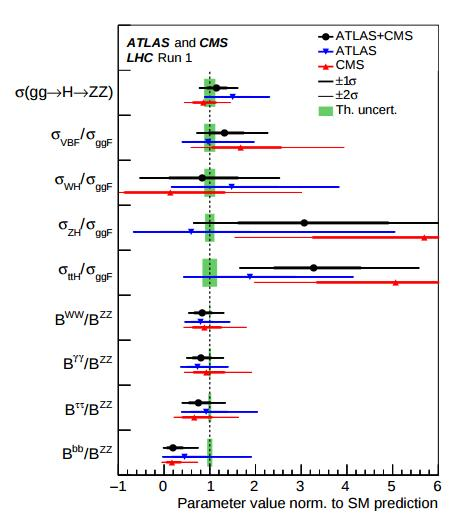
\includegraphics[width=0.7\textwidth]{higgscouplings.jpg}
\caption{Comparison of experimental and theoretical measurements of Higgs production and decay modes. The decay modes are expressed as ratios of the $H \rightarrow ZZ$ decay mode. \cite{Khachatryan:2016vau}}
\label{fig:higgsSMBR}
\end{figure}

\begin{figure}[here]
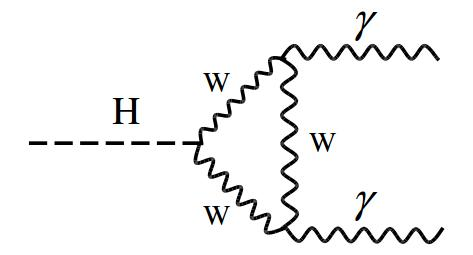
\includegraphics[width=0.7\textwidth]{higgswwgammagamma.jpg}
\caption{Production of $H \rightarrow \gamma \gamma$ via a virtual W boson loop. Analogous diagrams with top quark loops also contribute to the process.}
\label{fig:higgsgg}
\end{figure}

\qquad The four lepton final state signatures of the $H \rightarrow ZZ$ and $H \rightarrow \gamma\gamma$ channels were used to reconstruct the mass of the Higgs boson. The results are shown in figure \ref{fig:higgsmass}. 

\begin{figure}[here]
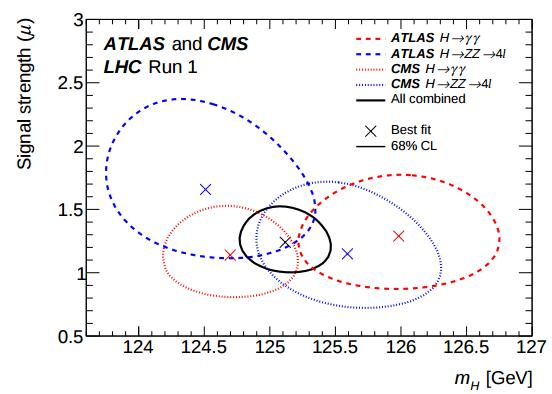
\includegraphics[width=0.9\textwidth]{higgsmass.jpg}
\caption{Results of Higgs mass measurements. The combined result is approximately 125 GeV \cite{Aad:2015zhl}}
\label{fig:higgsmass}
\end{figure}

\qquad As discussed in section \ref{higgstheory}, Higgs boson couplings are mass dependent. The more massive the particle, the stronger its coupling is to the Higgs. Top quarks, with a mass of 172 GeV, are the heaviest standard model particle. As a result, the dominant method of Higgs production is when two energetic gluons fuse together via a top quark loop, as shown in Figure \ref{fig:ggfHiggs}. This is called gluon-gluon fusion. The estimated cross section is 19.27 pb at $\sqrt{s} = $ 8 TeV and 43.92 pb at $\sqrt{s}$ = 13 TeV.

\begin{figure}[here]
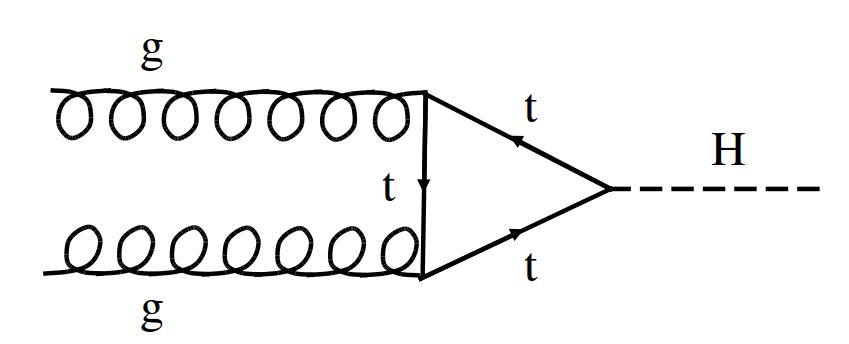
\includegraphics[width=0.9\textwidth]{ggfHiggs.jpg}
\caption{Higgs production via gluon gluon fusion.}
\label{fig:ggfHiggs}
\end{figure}


\qquad Vector boson fusion (VBF) is the second most likely method of Higgs boson production, with an estimated crosss section of 1.578 pb at $\sqrt{s}$ = 8 TeV and 3.748 pb at $\sqrt{s}$ = 13 TeV.
It is shown in Figure \ref{fig:vbfHiggs}. The two quarks that seed the jets are thrust apart in $\eta$ after vector boson radiation. This rapidity gap between the two highest $p_{T}$ jets in vector boson fusion allows us to distinguish this signal from events with a top quark and an antitop quark ($t\bar{t}$ events). The vector bosons that connect the final state quarks are colorless, and the final state jets will have no inherent strong force connection (section \ref{elemforces}). However, in $t\bar{t}$ (figure \ref{fig:ttbarcolor}) the top and antitop quarks will be connected at a gluon vertex. Because gluons are color doublets (section \ref{elemforces}) the two final state quarks may be color connected, meaning that they share the same color. If this is the case, then the increase in potential energy will cause central jet formation within the rapidity gap, distinguishing this background from the VBF Higgs signal. \ref{fig:higgsproduction}\cite{Dittmaier:2011ti}. The Higgs may also be produced in associated with a vector boson or in associated with two top quarks. These channels are essentially negligible in a $H \rightarrow \mu\tau$ search.

\begin{figure}[here]
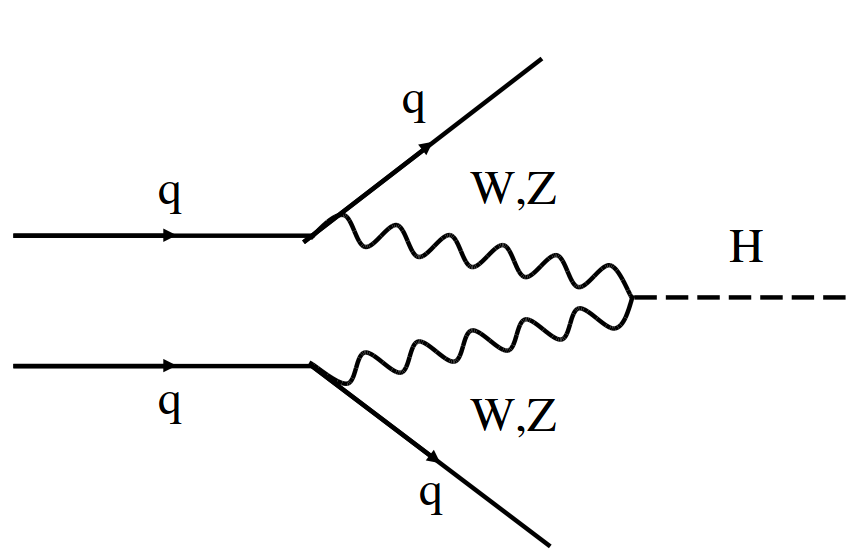
\includegraphics[width=0.9\textwidth]{vbfHiggs.png}
\caption{Higgs production via vector boson fusion.}
\label{fig:vbfHiggs}
\end{figure}

\begin{figure}[here]
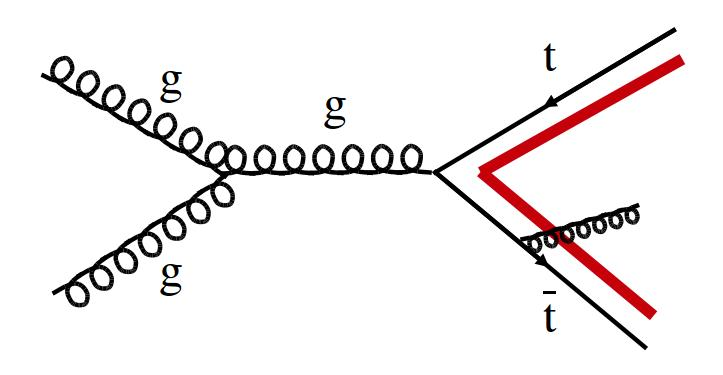
\includegraphics[width=0.9\textwidth]{ttbarcolor.jpg}
\caption{Color connected $t\bar{t}$ production. The bold (red) line indicates a color connection between the final state quarks. Central jets are beginning to form due to the increase in potential energy as the color connected quarks move apart.}
\label{fig:ttbarcolor}
\end{figure}

\begin{figure}[here]
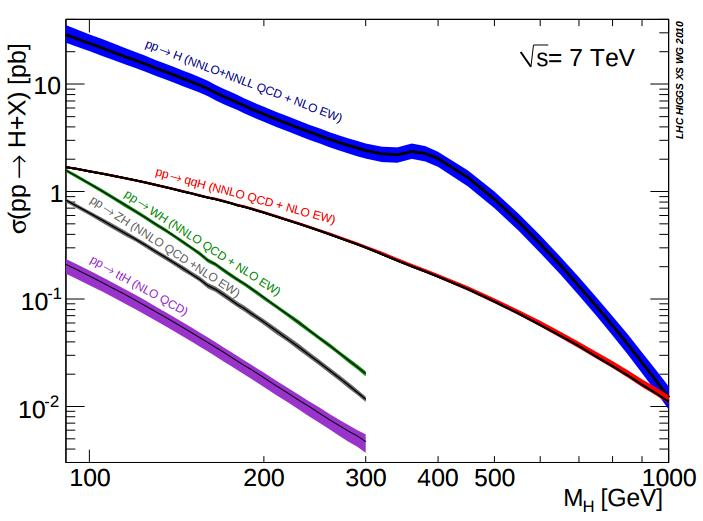
\includegraphics[width=0.9\textwidth]{higgsproduction.jpg}
\caption{Higgs production cross sections\cite{Dittmaier:2011ti}. At a mass of 125 GeV, the two most likely production modes are gluon gluon fusion and vector boson fusion.}
\label{fig:higgsproduction}
\end{figure}

\qquad There is no known Higgs branching ratio to guide this search. This is the first direct measurement of $H \rightarrow \mu \tau$. The kinematics of this search are similar to the kinematics $H \rightarrow \tau\tau$ search carried out at CMS \cite{Chatrchyan:2012xdj}. As discussed in section ~\ref{taus}, tau leptons are detected at CMS via their hadronic decay mode ($\tau_{h}$) or their leptonic decay modes ($\tau_{e}, \tau_{\mu}$). Therefore, the final state objects, a muon and a tau, are exactly the same between the $H \rightarrow \mu \tau$ and the $H \rightarrow \tau_{\mu} \tau$ channel of $H \rightarrow \tau\tau$, making $H \rightarrow \tau\tau$ a major background of the search. A significant difference between $H \rightarrow \tau_{\mu} \tau$ and $H \rightarrow \mu \tau$ is the distribution of missing transverse energy (MET) in the event. MET, which is discussed further in section ~\ref{met}, arises from neutrinos and other particles that CMS cannot detect. As shown in figure ~\ref{fig:TauDecay}, tau decays will always produce neutrinos. The $H \rightarrow \tau_{\mu} \tau$ channel will contain a muon neutrino associated with the muonic decay of the tau, but $H \rightarrow \mu \tau$ contains no such neutrino. The only neutrinos will be associated with the tau decay. The MET distribution will be used to define the signal region in section 6. A graphic of Higgs boson decay branching fractions is shown in Figure \ref{fig:higgsBR}\cite{Heinemeyer:2013tqa}

\begin{figure}[here]
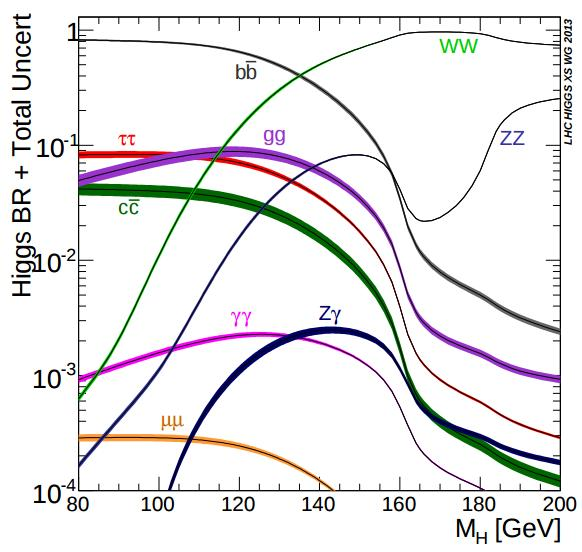
\includegraphics[width=0.9\textwidth]{higgsBR.jpg}
\caption{Higgs decay branching fractions\cite{Heinemeyer:2013tqa}. The mass of the Standard Model Higgs is 125 GeV. }
\label{fig:higgsBR}
\end{figure}



\chapter{Experimental Design}\label{experiment}

\section{LHC}\label{lhc}

\qquad The Large Hadron Collider (LHC) is a proton-proton collider located at CERN in Geneva, Switzerland \cite{1748-0221-3-08-S08001}. The LHC was designed to collide protons at a center of mass energy of 14 TeV. It has operated at a center of mass energy of 7 TeV in 2011, 8 TeV in 2012, and 13 TeV in 2015. The following paragraphs will explain how the LHC creates and collides its proton beams.

\qquad The protons used in LHC collisions begin the process as the nuclei of hydrogen atoms in a bottle of hydrogen gas. An electric field is applied, separating the protons and electrons in hydrogen. The protons are then accelerated through Linac 2 (figure \ref{fig:cernacc}) up to an energy of 50 MeV. Linac 2 uses radiofrequency (RF) cavities that create alternating electrical fields in conductors. These alternating fields continuously accelerate the protons along the beamline.

\begin{figure}[here]
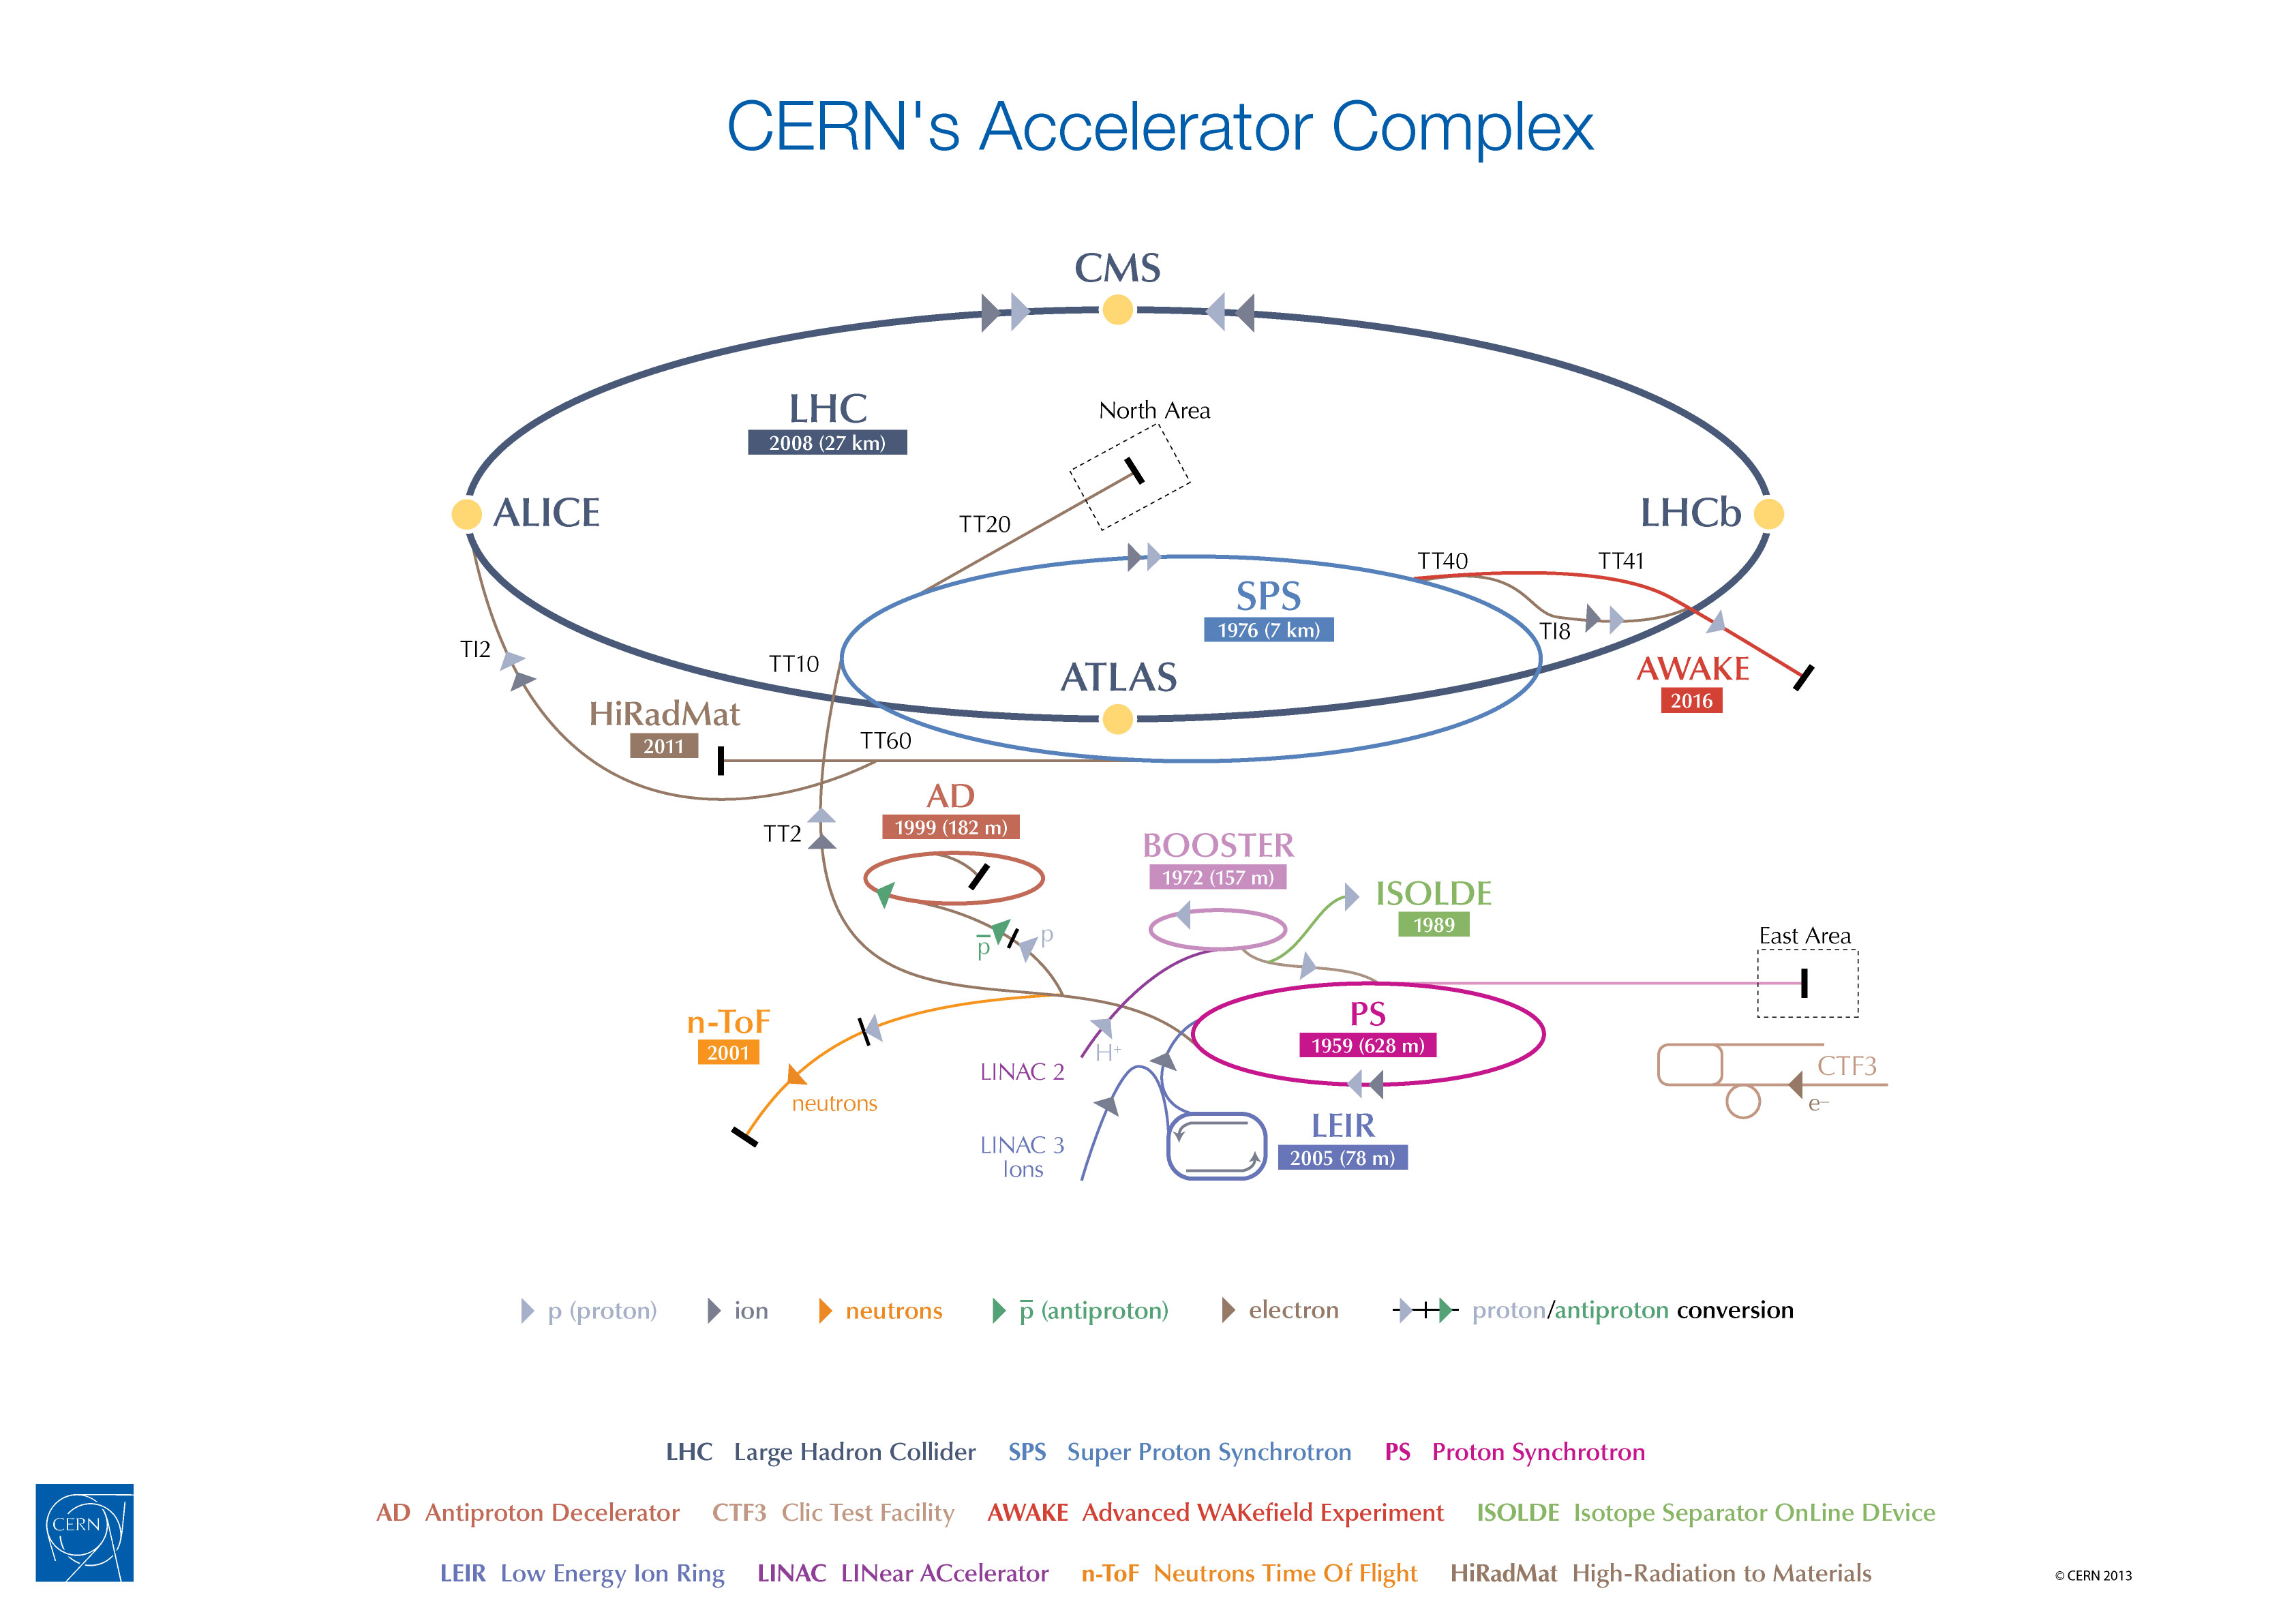
\includegraphics[width=0.9\textwidth]{CERN's-accelerator-complex2013.jpg}
\caption{The series of accelerators and experiments that make up CERN \cite{Marcastel:1621583}}
\label{fig:cernacc}
\end{figure}

\qquad The protons then enter the Proton Synchotron Booster (PSB), which accelerates them up to 1.4 GeV. The PSB accelerates the protons in a circle, using RF cavities in conjunction with dipole magnets to guide the circular path of the beam and quadropole magnets to focus the beam. The Proton Synchotron (PS) accelerates the protons up to 25 GeV, and finally the Super Proton Synchotron (SPS) accelerates the protons up to 450 GeV, preparing them for their arrival in the LHC.

\qquad After entering the LHC, the protons are further accelerated up to their intended collision energy. The first run, in 2011, accelerated the protons up to 3.5 TeV. This was increased to 4 TeV in 2012, and to 6.5 TeV in 2015. The two proton beams travel in opposite directions around the LHC ring, which is 27 km in circumference. Therefore, the center of mass energy of collisions is twice as much as the energy of the individual beams. The beams are crossed at points within each of the major LHC experiments, producing proton-proton collisions.

\qquad The beams in the LHC travel in opposite directions around the LHC in vacuum sealed beam pipes and are controlled using superconducting NbTi magnets, which are cooled down to below 2K using liquid helium. The magents are designed to produce a magnetic field of 8.3 T, which requires a current of 11850 A. Superconducting magnets are required so that the magnets don't act as resistors against the high current needed to sustain the high magnetic field. There are 1232 dipole magnets, which bend the beams in their circular paths, and 392 quadropole magnets, which keep the beams focused. The beam is accelerated by RF cavities operating at a frequency of 400 MHz.

\qquad The protons in the beam are divided up into ``bunches". Each bunch contained about $1.7 \times 10^{11}$ protons in 2012 and about $1.1 \times 10^{11}$ protons in 2015. In 2012, the LHC ran with 1374 bunches per beam, with 50 ns spacing in between bunches. In 2015, the number of bunches per beam was gradually increased up to 2244 bunches per beam, with 25 ns bunch spacing. However, the intensity of the beam was lower in 2015 than in 2012. The transverse emittance ($\epsilon$) is a measure of the beam's cross sectional area in its phase space. It was 1.8 $\mu$m in 2012 and about 3 $\mu$m in 2015. The $\beta$ function in accelerator physics relates the transverse emittance to the cross section area of the beam ($\sigma_{x}\sigma_{y}$) via: $ \beta	= \sigma_{x}\sigma_{y} / \epsilon$. The value of the $\beta$ function at the interaction point is referred to as $\beta^{*}$, which has increased from 0.6m in 2012 to 0.8m in 2015.

\qquad The performance of the LHC can be measured by how many proton proton collisions it creates. The number of events generated per second at the LHC ($N$) is given by: $N = L\sigma$, where $\sigma$ is the proton-proton cross section (section \ref{ppcoll}) and $L$ is the luminosity. The luminosity is proportional to the square of the number of particles per bunch, the number of bunches, and the revolution frequency of 11.2 kHz, and inversely proportional to $\epsilon$ and $\beta^{*}$. The peak luminosity delivered to CMS by the LHC in 2012 was $7 \times 10^{33} s^{-1} cm^{-2}$, and at 2015 it was $5.33 \times 10^{33} s^{-1} cm^{-2}$. While 2016 data is not contained in this thesis, the LHC performance has improved significantly. The luminosity is currently at $1.0 \times 10^{34} s^{-1} cm^{-2}$, which has been achieved by decreasing $\beta^{*}$ to 0.4m.


\section{CMS}\label{cms}
\subsection{Overview}

\qquad The Compact Muon Solenoid (CMS) detector is a mostly hermetic detector at the LHC that is responsible for detecting the hadrons, photons, and charged leptons in an event after the proton-proton collisions \cite{1748-0221-3-08-S08001}. CMS contains a superconducting magnet which produces a 3.8T magnetic field along the beamline. The innermost component, the tracker, measures the trajectory of all charged particles in the event. The electromagnetic and hadronic calorimeters measure the energy deposits of electrons, photons, and hadrons in the event. Muons are highly penetrating particles, so the muon system must reside furthest from the interaction point, outside the magnet. The iron yoke in the muon system responds to the magnetic flux of the 3.8 T magnet and creates a 2 T magnetic field, allowing the $p_{T}$ of the muons to be measured. A cross section of CMS is shown in figure \ref{fig:cmsxsec}. 

\begin{figure}[here]
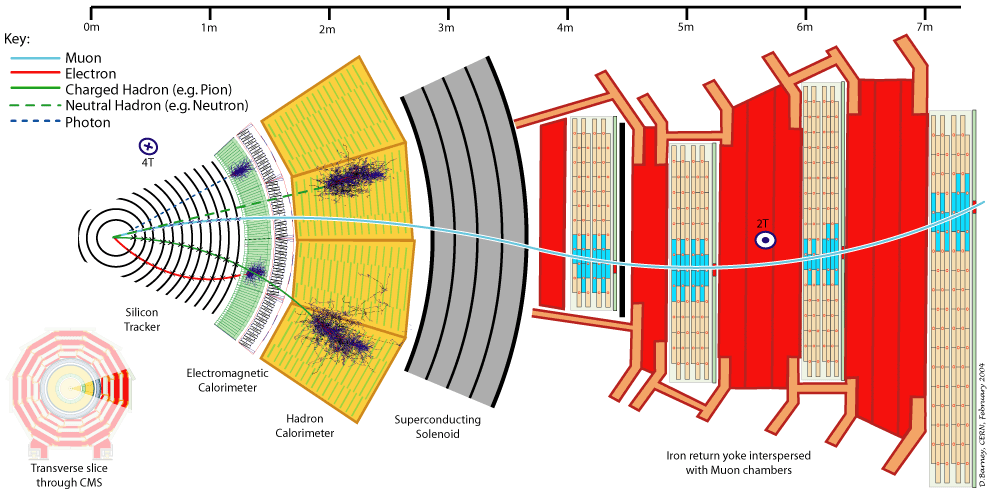
\includegraphics[width=0.9\textwidth]{CMS_SLICE.png}
\caption{An illustration of the passage of particles through the CMS detector. \cite{CMS_SLICE}}
\label{fig:cmsxsec}
\end{figure}

\qquad A diagram of CMS's geometry is in figure \ref{fig:cmscoord}. The $z$ direction points along the beamline and the $x-y$ coordinate system is perpendicular to the beamline, with the $x$ axis pointing towards the center of the LHC. The azimuthal angle in the $x-y$ plane is $\phi$ and the polar angle with respect to the $z$ axis is $\theta$. The lorentz invariant quantity $\eta$ (pseudorapidity) is commonly used in place of $\theta$, where $\eta = ln(tan(\theta/2))$.

\begin{figure}[here]
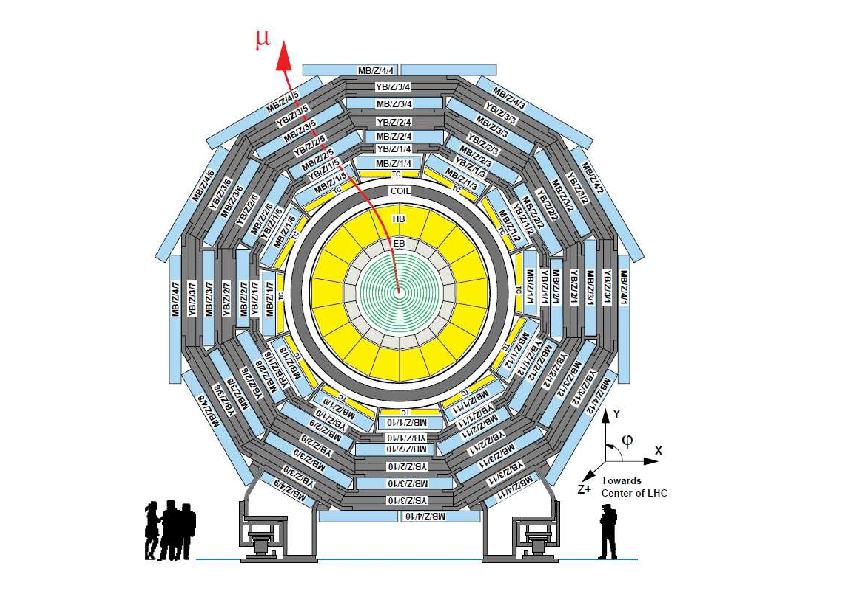
\includegraphics[width=0.9\textwidth]{CMSview.png}
\caption{A cross section of CMS, showing the trajectory of a muon. The coordinate system is in the lower right hand corner. \cite{Chatrchyan:2009hg}}
\label{fig:cmscoord}
\end{figure}

\subsection{Tracker}\label{tracker}

\qquad The tracking system was built to provide accurate measurements of the trajectories of charged particles.  A charged particle in a magnetic field will move in a circle of radius $R = qBp_{T}$, where $q$ is the charge, $B$ is the magnetic field, and $p_{T}$ is the momentum transverse to the magnetic field. Therefore, by reconstructing the trajectories of charged particles, we can determine their radius of curvature and hence their momentum. The tracker also enables us to determine if particles originated from primary or secondary vertices.

\qquad The tracker has two major components: an inner pixel detector and an outer silicon strip tracker. The pixel detector has three layers, at 4.4, 7.3, and 10.2 cm from the beamline. The silicon strip tracker has 10 layers extending to a radius of 1.1 m. Endcaps in each system extend the range in $\eta$ out to 2.5. There are 1440 pixel modules and 15148 silicon strip modules. The radiation length of the tracker varies as a function of $\eta$, as shown in figure \ref{fig:trackerlength}. A laser alignment system with a wavelength of 1075 nm is regularly used during data taking to check the position of the tracker. The system can monitor movements down to 10$\mu m$. 

\begin{figure}[here]
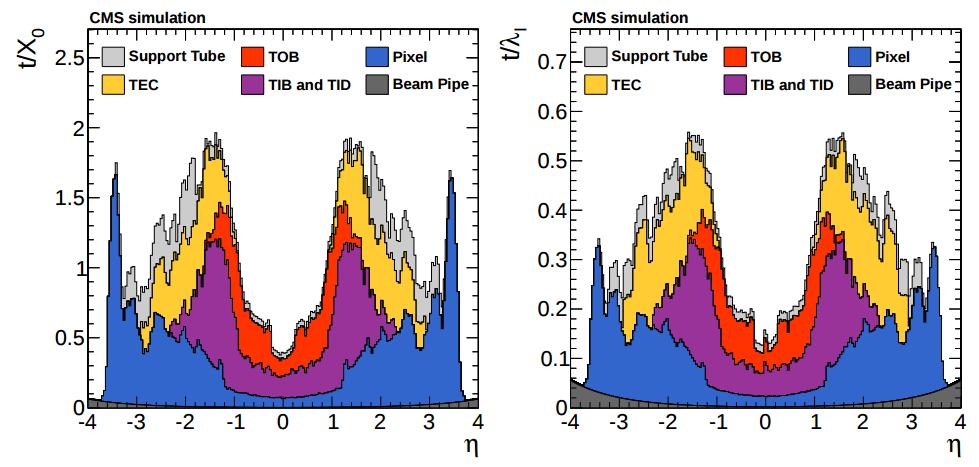
\includegraphics[width=0.9\textwidth]{trackerlength.jpg}
\caption{Width of the tracker in unites of radiation length (left) and nuclear interaction length (right) \cite{Chatrchyan:2014fea}}
\label{fig:trackerlength}
\end{figure}


\qquad A high resolution pixel detector is necessary to deal with the high particle flux close to the beamline.  At the design luminosity of $10^{34} cm^{-2} s^{-1}$, the pixel detector must withstand a hit rate density of 1 MHz/$mm^{2}$ at its inner radius of 4.4 cm. The high rate requires the use of pixelated detectors close to the beamline. The pixel sensors are rectangles of size $100 \times 150 \mu m^{2}$. The resolution in the pixel detector is about 20 $\mu$m in the radial direction and 25$\mu$m in the longitudinal direction\cite{Meier:1977837}. This degree of resolution allows the pixel detector to detect displaced secondary vertices from the decay of B hadrons, as discussed in section \ref{bjets}. The pixel detector is divided into two components: the barrel layers (BPix) and the endcap disks (FBix). The BPix contains 48 million pixel sensors while the FPix contains 18 million.

\qquad The pixel sensors are n+ doped and are bonded to an n doped substrate, with a pn junction on the backplane of the substrate. This means that both the pixel sensors and the substrate have more electrons that holes, but the electron to hole ratio is higher in the pixel sensor than in the substrate. When a charged particle passes through the substrate, it causes a cascade of electrons to move towards the pixels, creating an electrical impulse. Readout chips, which amplify the signal, are bump bonded \cite{Chiochia:2007pu} to the pixel sensors. The Token Bit Manager (TBM) chip controls the readout of groups of pixel sensors. It is connected via optical fibers to the data acquisition system (DAQ) and requires the pixel output to be synchronized with the trigger.

\qquad Further from the beamline, the lower flux of particles permits the use of silicon micro-strips of size $10 cm \times 80 \mu m$ between 20 cm $< r < $ 55 cm and size $25 cm \times 180 \mu m$ in the region 55 cm $ < r < $ 110 cm. The microstrips are n-p silicon sensors, and there are 9.3 million in total. The inner barrel of the silicon strip tracker contains four cylinders which are 25.5 cm, 33.9 cm, 41.85 cm, and 49.8 cm away from the beam axis. The barrel extends in the z direction from +70 cm to -70 cm. To extend the range in $\eta$, inner disks of the tracker are placed in groups of three in between $\pm$80 cm and $\pm$90 cm in the z direction. This setup gives coverage throughout the $\eta<$  2.5 region.

\qquad The outer barrel of the tracker consists of a wheel with 688 rods, which support the silicon strips. The rods with the silicon detectors are inserted into the wheel at radii of 60.8 cm, 69.2 cm, 78.0 cm, 86.8 cm, 96.5 cm and 108.0 cm. The rods are angled such that they overlap in $\phi$ and provide full coverage in each layer.

\qquad The tracker endcaps extend the range of the tracker in the $z$ direction, from $\pm$ 124.0 cm to $\pm$ 280.0 cm. They also cover the radial range of 22.0 cm to 113.5 cm. Each endcap consists of nine circular discs, and each disc holds 16 petals, which are structures that hold modules of silicon sensors. The modules are angled to overlap and give full coverage in $\phi$. A full schematic of the tracker is show in figure \ref{fig:cmstracker}.

\begin{figure}[here]
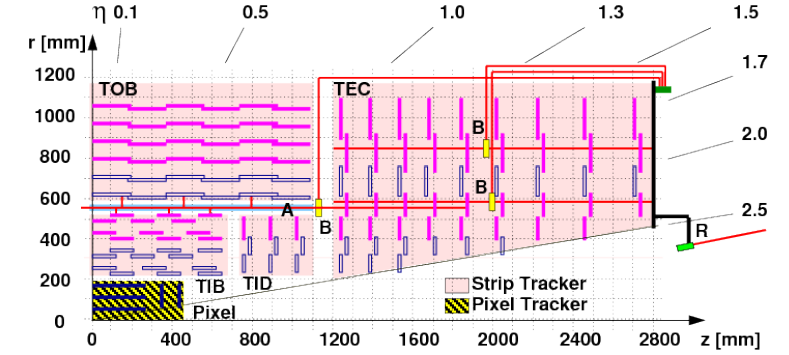
\includegraphics[width=0.9\textwidth]{cmstracker.png}
\caption{Layout in $r$, $\eta$, and $z$ of the CMS tracker and its components.  \cite{Chatrchyan:2014wfa}}
\label{fig:cmstracker}
\end{figure}

\subsection{ECAL}\label{ecal}

\qquad The electromagnetic calorimeter (ECAL) is a mostly hermetic homogeneous hermetic calorimeter that measures the energy deposits from electrons and photons. The calorimeter is composed of approximately 68000 crystals in the barrel and endcaps. A drawing of the ECAL is shown in figure \ref{fig:cmsecal}.

\begin{figure}[here]
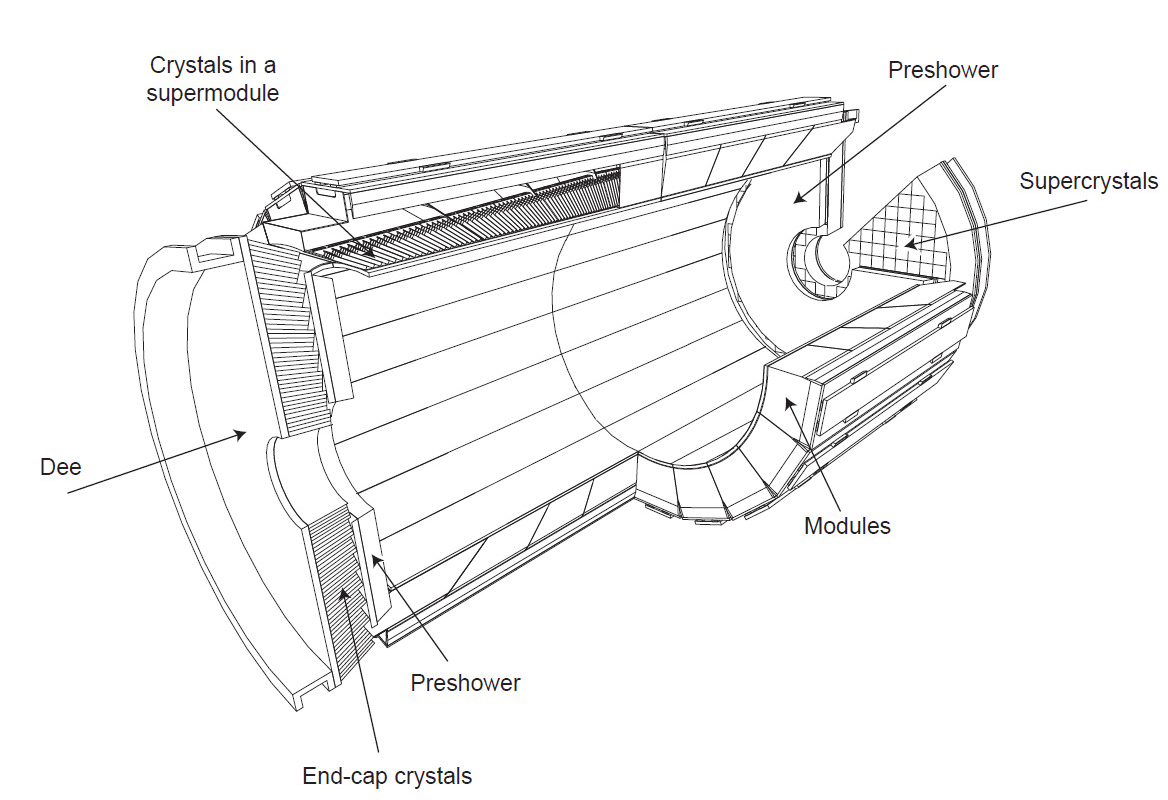
\includegraphics[width=0.9\textwidth]{cmsecal.png}
\caption{Diagram of the ECAL\cite{1748-0221-3-08-S08001}.}
\label{fig:cmsecal}
\end{figure}

\qquad The lead tungstate crystals are well suited for the ECAL. The crystals are have a high density of 8.28 $g/cm^{3}$, a short radiation length of 0.89 cm, and small Moliere radius of 2.2 cm. The radiation length is defined as the mean distance for an electron's energy to decrease by $1/e$. The Moliere radius is defined as the radius of a cylinder that contains 90\% of the electron shower's radiation. The density, radiation length, and Moliere radius of the lead tungstate crystals allows the ECAL to be compact and have high granularity. The crystals respond to the passage of electrons and photons by emitting blue/green scintillation light at a wavelength of 420-430 nm. The crystals emit 80\% of their scintillation light in 25 ns, which corresponds well to the design 25 ns bunch spacing of the LHC, as discussed in section \ref{lhc}. The crystals are radiation resistant, but do have a limited tendency to develop defects when exposed to radiation. These defects will absorb the scintillated light. The crystal behavior is also very sensitive to temperature. Corrections for these irregularities are determined by applying laser pulses with a known intensity to the crystals and measuring the response.

\qquad The barrel of the ECAL (EB) contains 61,200 crystals and covers the range $|\eta| < 1.4442$. The crystals are angled slightly to avoid creating cracks in the ECAL. The crystals cover an area in the $\eta - \phi$ plane of $0.0174 \times 0.0174$. The barrel has a radial depth of 25.8 radiation lengths, which corresponds to 23.0 cm. The crystals are grouped into modules which have an $\eta$ dependent geometry and each contain 400-500 crystals. A supermodule is made up of four modules and contains 1700 crystals. There are 36 supermodules in EB. The scintillation light from each crystal is detected with avalanche photodiodes (APD), which are mounted to the backs of crystals in pairs. A diagram of an APD is shown in figure \ref{fig:APD}. 

\begin{figure}[here]
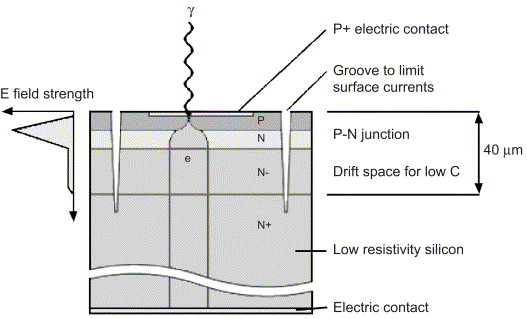
\includegraphics[width=0.9\textwidth]{apd.jpg}
\caption{Operation of an APD in the EB  \cite{Brown:2007cg}}
\label{fig:APD}
\end{figure}

%The APDs are operated at a gain of 50.

\qquad The endcaps of the ECAL (EE) cover the range $1.566 < |\eta| < 2.5$. Each endcap has two disc shaped mounts (Dee's) for the crystals. The crystals in each Dee are supported in units of 5x5 crystals which are called supercrystals. The supercrystals are arranged rectangularly on each Dee in an x-y grid. Each crystal has a length of 22.0 cm, corresponding to a radiation length of 24.7. There are about 14500 crystals total in the EE. The scintillation light is amplified by vacuum phototriodes (VPT). VPTs are used in the endcap due to their ability to withstand the large hadron flux in the forward region. A schematic of a VPT is show in figure \ref{fig:VPT}.

\begin{figure}[here]
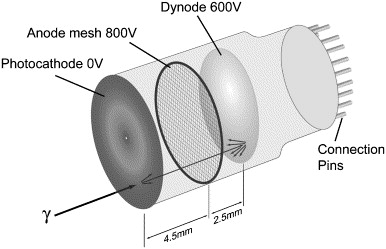
\includegraphics[width=0.9\textwidth]{vpt.jpg}
\caption{Schematic of a VPT in the EE  \cite{Brown:2007cg}}
\label{fig:VPT}
\end{figure}

\qquad The detector electronics reads the output of a trigger tower (5 x 5 crystals) and generates digital $E_{T}$ sums that are sent to the L1 trigger (section \ref{trigger}) every bunch crossing.

\qquad The energy resolution of the ECAL is given by 

\begin{equation}
\label{eq:ecal}
\left(\frac{\sigma_{E}}{E}\right)^{2} = \left(\frac{A}{\sqrt{E}}\right)^{2} \oplus \left(\frac{B}{E}\right)^{2} \oplus \left( C \right)^{2}
\end{equation} 


In equation \ref{eq:ecal}, there are three experimentally determined terms. $A$ is a stochastic term that takes energy fluctuations into account. It is determined to be 2.8\%. $B$ is a noise term representing noise from the electronics and pileup. It is 0.12. $C$ is a constant term that represents the uniformity and stability of the ECAL. It is measured to be 0.3\%. 

\qquad There is an additional component of the ECAL called the Preshower. It is located in front of the ECAL for $1.653 < |\eta| < 2.6$. the preshower consists of silicon strip detectors located behind 2 radiation lengths, plus an additional radiation length of lead absorber \cite{Cockerill:2008td}. The preshower is used to discriminate against boosted $\pi^{0}$'s, which decay into photon pairs. If the $\pi^{0}$ is sufficiently boosted the photon pairs may not be resolved properly in the ECAL and the $\pi^{0}$ will be reconstructed as one photon. The preshower is able to resolve these events, thus reducing a significant background to diphoton analyses.


\subsection{HCAL}\label{hcal}

\qquad The hadronic calorimeter (HCAL) is designed to detect hadronic energy deposits, such as jets. It consists of four components: the barrel (HB), endcap (HE), a forward region that covers high $|\eta|$ (HF), and an outer region designed to detect energetic hadronic showers (HO).

\qquad HB covers the region $|\eta| < 1.3$. It has 14 layers of brass absorber mounted between steel front and back plates. Brass was chosen due to its short interaction length and lack of magnetic behavior. The thickness of the HCAL is measured in interaction lengths, which is the mean distance for a hadronic particle to travel before undergoing inelastic scattering with a nucleus. HB ranges from 5.8 interaction lengths at $\eta = 0$ to 10.6 interaction length at $|\eta| < $1.3.  Trays of plastic scintillator are inserted between layers of the brass absorber. Hadrons interact with the brass, losing energy and producing electromagnetic showers. These showers produce light in the plastic scintillator, which is read out via wavelength shifting fibers connected to hybrid photodiodes. HE covers the region $1.3 < |\eta| < 3.0$ and also extends for a length of 10 interaction lengths.

\qquad The HF covers the region $3.0 > |\eta| < 5.0$. This is a high radiation region, and HF must be particularly radiation hard. Instead of brass absorber and plastic scintillator, HF uses steel absorber and quartz fibers. The steel plates are 0.5 cm thick and 165 cm (10 interaction lengths) long. Quartz fibers are inserted into the grooves 0.5 cm apart. There are two sets of fibers: one for identifying $e/\gamma$ showers and one for identifying hadronic showers. The $e/\gamma$ fiber set runs over the full length of the detector while the hadronic set starts 22 cm from the front of the detector, because the $e/\gamma$ showers deposit most of their energy in the first 22 cm. As the charged particles pass through the quartz fibers Cherenkov radiation is emitted, which is detected by photomultplier tubes (PMT). This extension of HCAL into the forward region significantly reduces the number of jets that leave CMS undetected. HF is necessary to detect jets with large $\eta$ separation, such as in Higgs boson production via vector boson fusion, as discussed in section \ref{higgspheno}. HF is also important for reconstructing the missing transverse energy. As discussed in section \ref{met}, the missing energy is reconstructed by examining momentum imbalances in CMS. If the visible decay products escape CMS, valuable information about the missing energy is lost. HF significantly improves the coverage of the detector, which in turn significantly improves the reconstruction of missing energy.

\qquad The HO portion of the HCAL is located just outside the CMS magnet, covering the region $|\eta| < 1.3$.  It complements HB by providing an additional three radiation lengths of material for detecting energetic hadronic showers. HO consists of five rings extending along the beam axis. Each ring consists of 72 sections, which in total provide full $\phi$ coverage. Each tile of HO matches a tile in HB. Like HB, the tiles of HO are made of plastic scintillator, and the light from the scintillator is read out with wavelength shifting fibers. During 2012 data taking, hybrid photodiodes were used to measure the output of HO, but they did not perform as expected, partly due to their proximity to the magnet. In 2015 they were replaced by silicon photomultipliers (SiPMs), which offered magnetic field insensitivity and higher gain\cite{Lobanov:2015jla}. 



\subsection{Muon System}\label{muonsys}
\qquad The muon system is located outside of CMS's magnet and located inside an iron yoke that returns the flux of the magnet, resulting in a magnetic field of 2T. The yoke also absorbs hadrons, thus increasing the efficiency of the muon system. In order to reach the outer muon stations, hadrons that have ``punched through" the HCAL must then travel through an additional 10 interaction lengths of iron. This means that there is only a .004\% chance that these hadrons will reach the outer muon station without scattering inelastically and distinguishing themselves from muons. The muon detectors are gas based in order to cover a large surface area. Muons are detected when they ionize the gas, resulting in showers of charge particles that induce an electrical current on high voltage electrodes. The muon system is located beyond 10 nuclear interaction lengths to greatly reduce hadronic punchthrough. Muon hits and track segments are reconstructed at an efficiency of 95-98\% \cite{Chatrchyan:2013sba}.

\qquad In the barrel ($|\eta| < 1.2$), drift tubes (DT) are used to track muons. The drift tubes are located in four stations, which are cylinders surrounding the beam line. The three inner chambers have 60 drift tubes and the outer chamber has 70 drift tubes. Muons passing through the drift tubes will ionize the gas mixture of 85\% Ar, 15\% CO$^{2}$. The maximum path of drift in the chamber is 2.1 cm, corresponding to a maximum drift time of 380 ns. The spatial resolution in the DTs is approximately 1 mm\cite{Chatrchyan:2013sba}. The anode wires are kept at a positive potential of 3600V while the electrode strips are kept at a negative potential of -1200V. Electrons will naturally flow to the higher potential, due to their negative charge. Any ionized electrons will flow away from the electrode to the anode wire, inducing a measurable current. A schematic of a drift tube is show in figure \ref{fig:drift_tube}

\begin{figure}[here]
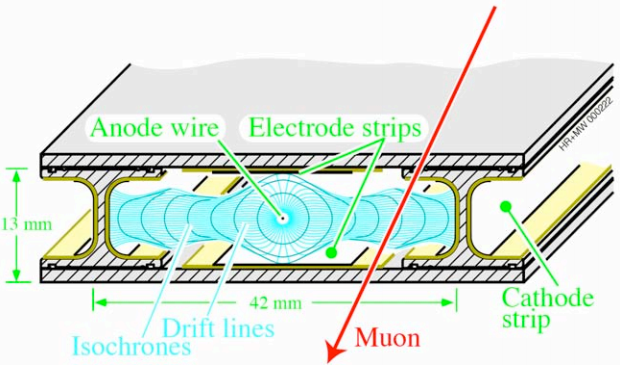
\includegraphics[width=0.9\textwidth]{drift_tube.png}
\caption{Schematic of a DT\cite{1748-0221-3-08-S08001}.}
\label{fig:drift_tube}
\end{figure}

\qquad In the endcap ($ 0.9 < |\eta| < 2.4$) muons are detected using cathode strip chambers (CSC). In 2012, there were 468 CSC's in CMS. This allowed for an endcap/barrel overlap region in $0.9 < |\eta| < 1.2$ where the muons are detected with DTs and CSCs. From $1.2 < |\eta| < 2.4$, each muon will cross 3-4 CSCs. As show in \ref{fig:muoncsc} each CSC has 7 layers of cathode strip panels, each separated by a gas gap filled with anode wires. There are about 400 wires per CSC. The gas mixture used is 40\% Ar, 50\% CO$_{2}$ and 10\% CF$_{4}$. Each wire is separated by 3.12 mm. The cathode strips extend in the radial direction, with a width that increases from 4 mm to 16 mm as the distance from the beam increases. The interpolation of the charge on consecutive cathode strips allows the $\phi$ position to be determined up to an uncertainty of 0.2 mm\cite{Collaboration:1355706} In preparation for 2015 running, new CSCs were added, increasing the number of CSCs from 468 to 540. The presence of the new CSCs fills a gap in the muon system where muons only passed through three layers of CSCs in 2012. Now all muons in the endcap will pass through four layers of CSCs, adding a layer of redundancy because only three hits out of four stations are required to identify potential muon candidates.

\begin{figure}[here]
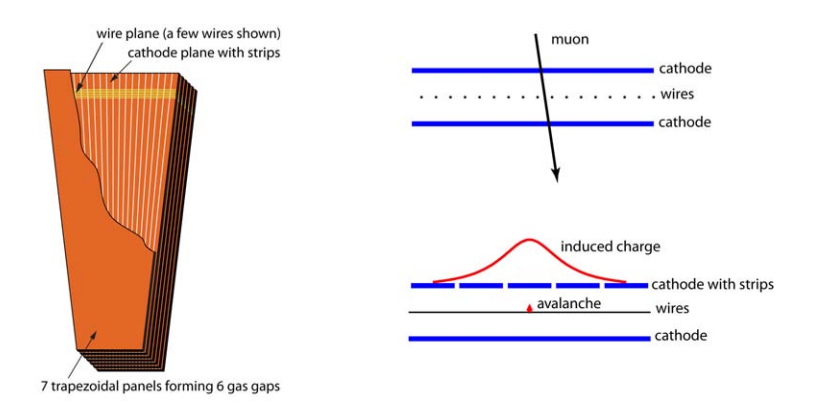
\includegraphics[width=0.9\textwidth]{muoncsc.png}
\caption{Schematic of a CSC (left) and an example of a CSC detecting and precisely determining the position of a muon (right).\cite{1748-0221-3-08-S08001}.}
\label{fig:muoncsc}
\end{figure}

\qquad In both the endcap and the barrel, resistive plate chambers (RPC) are used as a redundant trigger system. RPCs are gaseous parallel plate detectors that can identify the time of a muon track within 1 ns,  significantly faster than the 25 ns in between bunch crossings. The muon system identifies the correct bunch crossing in 99.5\% of events \cite{Chatrchyan:2013sba}. RPCs consist of two resistive plates 2mm apart with a gas gap in between. Muons will ionize the gas, which will cause a current to flow in detecting pads on the resistive plates. The spatial resolution of the RPCs is 1.2 cm\cite{Chatrchyan:2013sba} In total, 480 RPCs are in CMS, extending 245.5 cm along the beamline. In 2012 the RPCs extended up to $|\eta| < 1.6$. By 2015, additional RPCs were built, extending the system in the endcaps up to $|\eta| < 2.1$.

\subsection{Trigger}\label{trigger}
\qquad The CMS trigger system selects potentially interesting physics events among the hundreds of millions of proton-proton collisions per second. The Level 1 (L1) trigger takes inputs from the calorimeters and muon system to reduce the event rate to 100 kHz. Events that pass the L1 trigger are selected for further processing in the  High Level Trigger (HLT), which reduces the rate further to 1 kHz.

\qquad The L1 trigger reads events from the detectors at a rate of 40 MHz. The goal of the L1 trigger is to quickly accept or reject events which may contain promising physics by examining basic detector information, such as energy sums in the ECAL and HCAL. The L1 trigger accepts or rejects events within 4 $\mu$s. A flow chart for the L1 trigger is shown in figure \ref{fig:L1Trigger}. The L1 trigger is divided into two parts: the calorimeter trigger and the muon trigger. 

\begin{figure}[here]
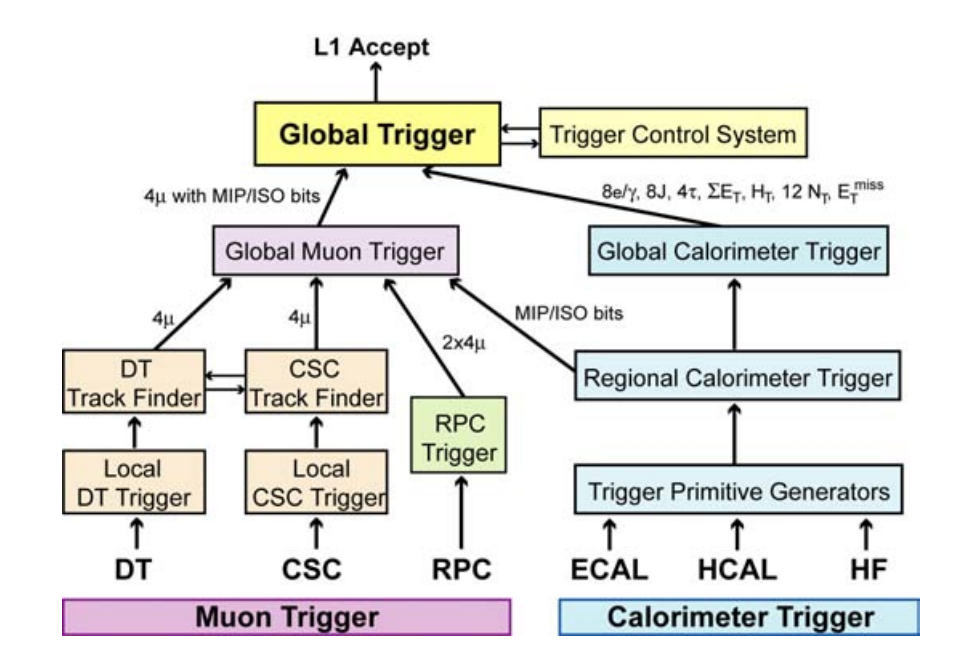
\includegraphics[width=0.9\textwidth]{L1trigger.png}
\caption{Workflow of the L1 trigger. The Global Muon Trigger returns the leading four muon candidates while the Global Calorimeter Trigger returns electron, jet, and tau canddiates as well as energy sums.\cite{1748-0221-3-08-S08001}}
\label{fig:L1Trigger}
\end{figure}

\subsubsection{Level 1 Trigger}\label{L1trig}

\qquad The L1 calorimeter trigger consists of the regional calorimeter trigger (RCT) and the global calorimeter trigger (GCT). The regional calorimeter trigger contains 4176 trigger towers. Of these trigger towers, 3456 are mapped to regions of 5x5 crystals in the ECAL and the corresponding single readout towers in the HCAL. Each trigger tower in the central region ($|\eta| < 3.0$) covers a region of 0.087 $\times$ 0.087 in the $\eta - \phi$ plane. Sums from ECAL and HCAL are computed in 4x4 regions of trigger towers. For $3.0 < |\eta| < 5.0$, only HF contributes sums. The RCT is detailed in figure \ref{fig:rct}.The trigger regions in this regime have the same granularity in $\phi$ (0.348), but a coarser granularity in $\eta$ (0.500). The $E_{T}$ sums from HF are simply passed on to the GCT. ECAL and HCAL each send 8 bit compressed $E_{T}$ sums along with a fine grain bit that indicates if 90\% ECAL energy in a trigger tower is restricted to a 2x5 crystal region in $\eta - \phi$. The RCT performs regional sums of the ECAL and HCAL energies and stores an H/E bit for an electron isolation, indicating if the HCAL energy is less than 5\% of the ECAL energy. Electron/photon candidates are constructed from 2x1 trigger towers.The RCT then identifies one isolated $e/\gamma$ candidate and one non-isolated $e/\gamma$ candidate per 4x4 trigger tower region. The jet/summary card sorts the four highest energy isolated and nonisolated candidates and passes them on to the GCT. 

\begin{figure}[here]
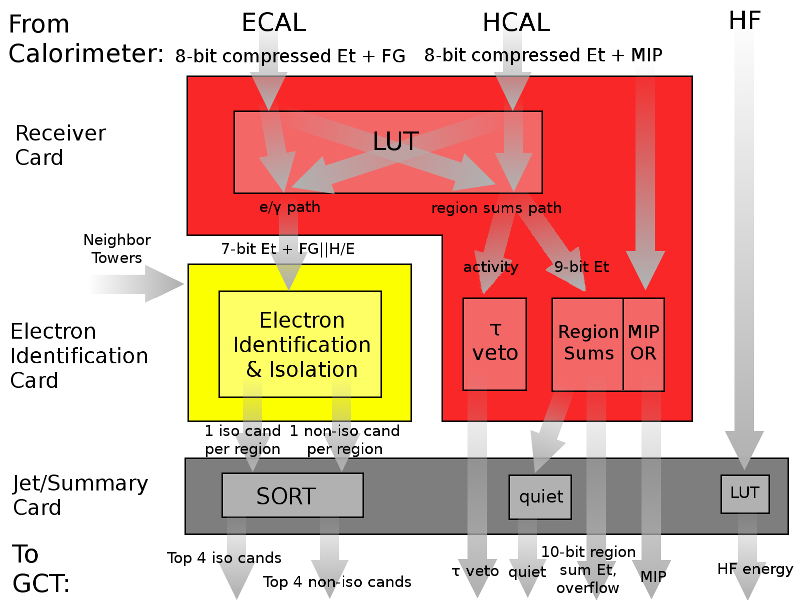
\includegraphics[width=0.9\textwidth]{rct.png}
\caption{Object reconstruction and transfer sequence associated with the RCT.}
\label{fig:rct}
\end{figure}

\qquad The RCT also calculates a tau veto bit for each 4x4 region, which requires the tau candidate to deposit its energy in a compact configuration of trigger towers, as shown in figure \ref{fig:tauveto}. The tau veto bit and the HCAL and HF $E_{T}$, $H_{T}$ (hadronic transverse energy) and MET sums are also passed on to the GCT, as shown in figure \ref{fig:rct}. The GCT uses this information to compute the four highest energy central jets, forward jets, taus, and MET. In 2012, taus and jets were identified in 12x12 trigger tower regions. The tau veto bit requirement was applied to each of the 4x4 regions in the 12x12 tau. The object was only identified as a tau and sent to the GCT if each 4x4 region passed the tau veto bit requirement. This information is sent to the global trigger, where it is combined with information from the global muon trigger, and the event is the accepted if it passes a L1 trigger cut, or vetoed and thrown away if it does not. This information is used to select physics events. 

\begin{figure}[here]
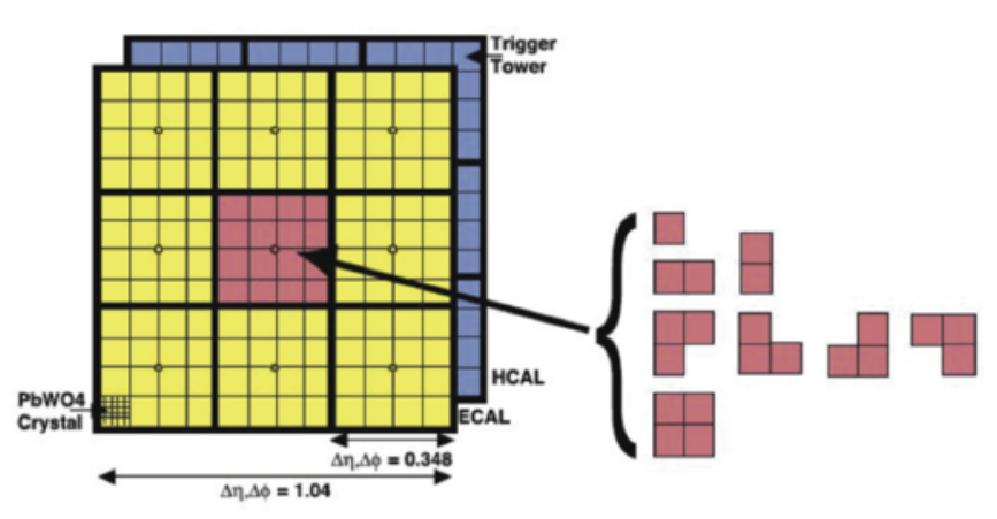
\includegraphics[width=0.9\textwidth]{tauveto.jpg}
\caption{For each 4x4 trigger tower region, the individual trigger towers where the ECAL or HCAL energy is above 3 GeV are examined. If they form one of the seven shapes on the right of the figure, the 4x4 region passes the tau veto. Taus deposit their energy in a smaller region than jets, so all 4x4 regions in the tau candidate are required to pass the tau veto selection\cite{CMS-DP-2015-009}.}
\label{fig:tauveto}
\end{figure}

\qquad An upgrade to the calorimeter trigger was introduced for 2015 data taking. The GCT was replaced by new electronics, and a new interface was added for the existing RCT. Existing copper wires linking the RCT to the GCT and ECAL were replaced by optical links. The oRSC (optical regional summary card) was developed by Wisconsin engineers to convert the RCT output to an optical format. The upgrade allowed for improved pileup subtraction algorithms that made the jet energies roughly pileup independent, as well as improved algorithms for taus. Taus are built from groups of 4x8 trigger towers and were dynamically constructed, combining a 4x4 trigger tower region with its highest energy non diagonal neighbor. The improvement in tau efficiencies from 2012 to 2015 is shown in figure \ref{fig:2012to2015taus}. The isolated taus are required to have roughly 90\% of the energy in the 12x12 trigger tower region centered on the tau to fall in the 4x8 region.

\begin{figure}[here]
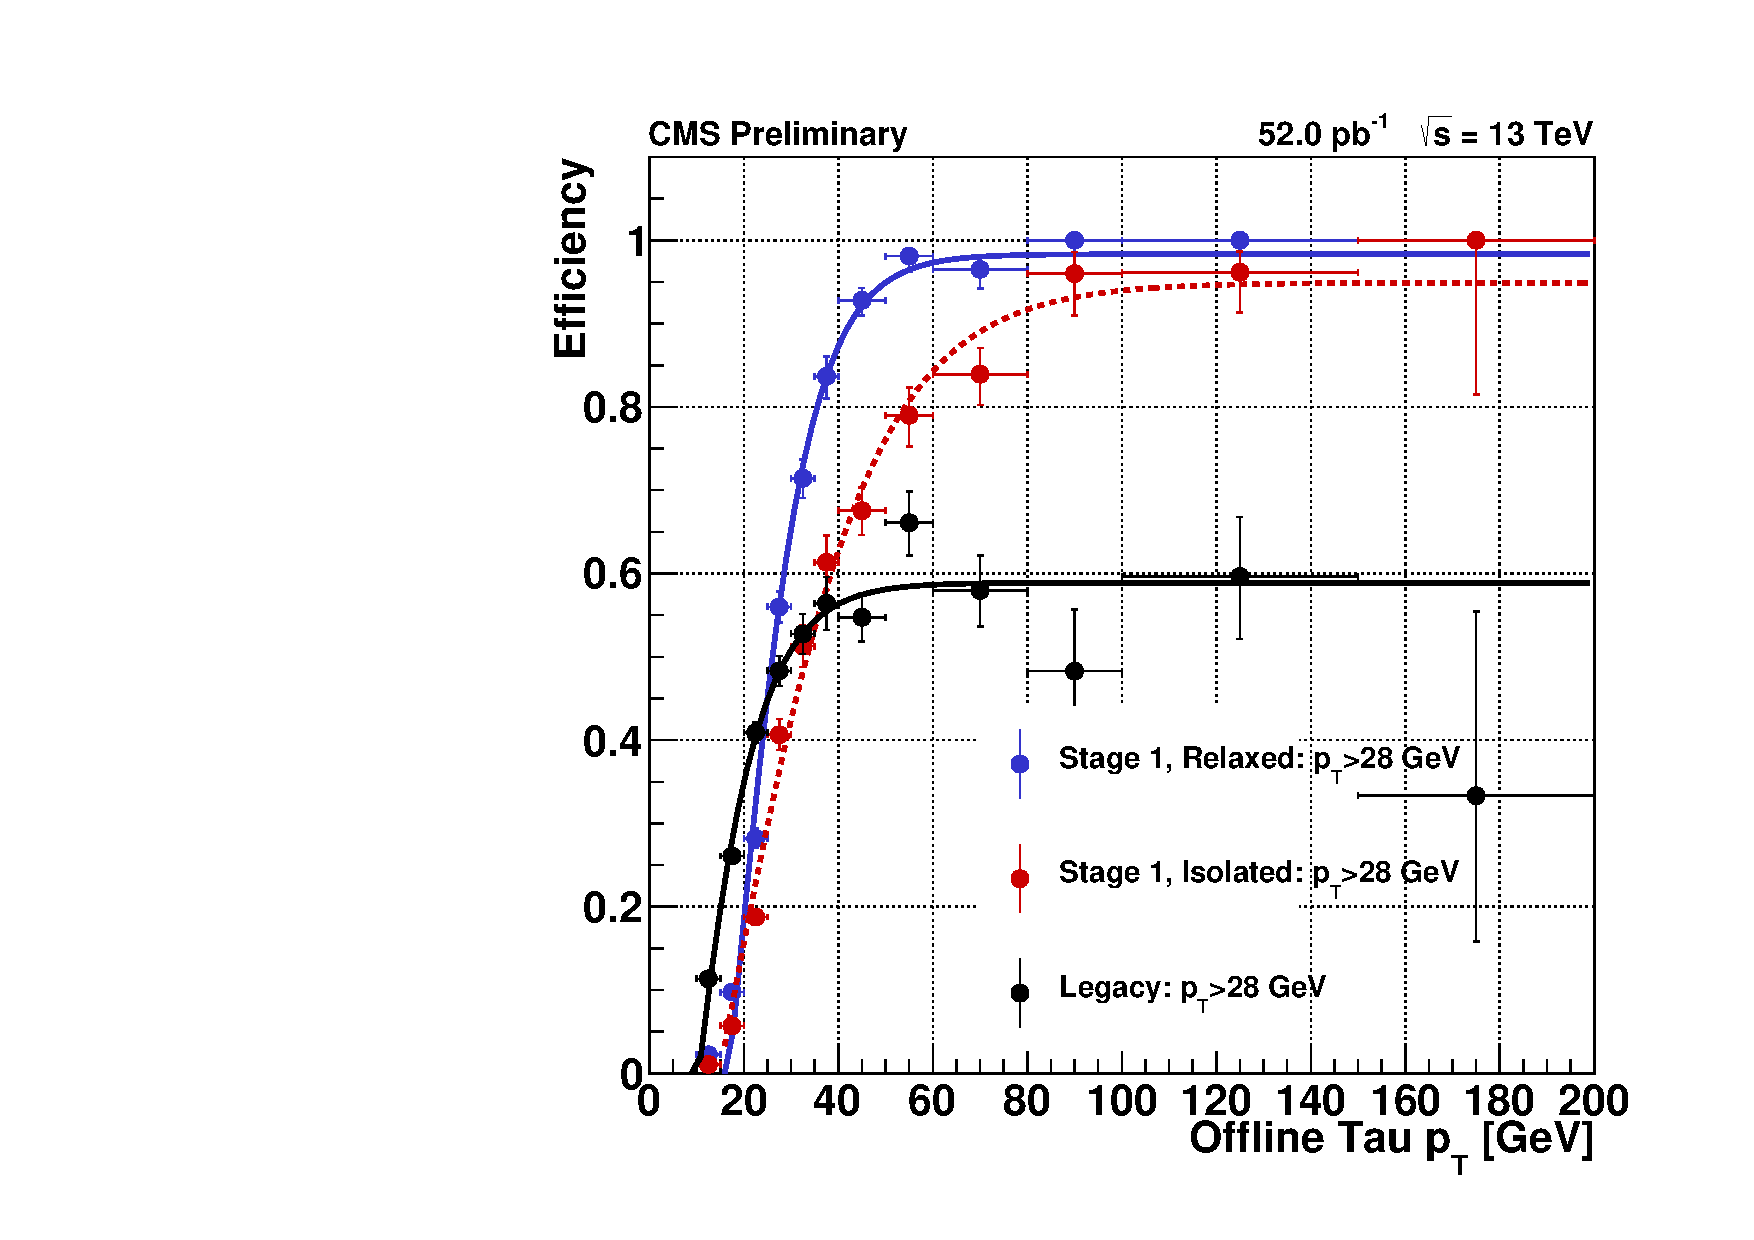
\includegraphics[width=0.9\textwidth]{TDR_RlxIsoLegacy_28GeV.pdf}
\caption{Stage 1 taus (2015) compared with GCT taus (legacy), using 2015 data. The legacy efficiency plateaus at about 60\%. The dynamical 4x8 construction of the Stage 1 taus improves the efficiency plateau to almost 100\%, reaching 80\% at a $p_{T}$ of 60 GeV.}
\label{fig:2012to2015taus}
\end{figure}

\qquad The Global Muon Trigger (GMT) takes inputs from the DTs, CSCs, and RPCs. The DTs and CSCs have associated track finders. They both build the four best muon candidates from the event and pass them on to the GMT. The RPC pattern comparator selects four muon candidates from the barrel and four from the endcaps, and sends the information to the GMT. The GMT then combines the information from the DTs, CSCs, and RPCs to build the four leading muon candidates in the event. 

\subsubsection{High Level Trigger}
\qquad Events that pass the L1 trigger are sent to the High Level Trigger (HLT) for further analysis. The  events passing the L1 trigger are read out at full granularity, including the tracker data, and are reconstructed much more carefully at the HLT level than they were by the L1 trigger algorithms. The detector data for each event that passed the L1 trigger is sent to a large computing farm with over 13,000 CPUs for the extensive HLT processing. The computing area is located above ground next to the CMS detector to minimize transfer time. Each HLT trigger has an associated path, which is a detailed series of instructions that reconstructs objects using the full detector information before applying the trigger. Both LFV Higgs and W+jets have a final state muon. Because muons are reconstructed with high efficiency at CMS, as mentioned in section \ref{muons}, we choose events passing the muon HLT triggers, which have almost 100\% efficiency.


\chapter{Event Simulation}\label{eventsim}
\qquad Particle interactions at CMS are computationally intensive to model. The strong nuclear force plays a dominant role in proton-antiproton collisions, but calculations involving QCD depend on large numbers of terms 
that define interactions between many quarks and gluons. At short distances, on the order of a femtometer, we can define the momentum scale $Q$ to be much greater than $\Lambda_{QCD}$, as defined in section \ref{elemforces}  This means that the effects of QCD can be calculated perturbatively (pQCD), which means that high order terms can be neglected and the calculations can be simplified. However, there are large amounts of soft radiation at $\Lambda_{QCD}$, as explained in section \ref{ppcoll}, which necessitates the use of computational software.

\qquad The interactions of the collision products with the the detector also need to be modelled via simulation. Accurate models of physical processes at CMS are vital for testing existing theories and searching for new ones, so accurate modelling of these processes is very important for CMS and for particle physics in general.
   
\section{Monte Carlo Event Generation}\label{mcgen}
\qquad Physical processes at CMS are simulated using a class of software called Monte Carlo generators. These programs are named after the location of the famous casino because Monte Carlo software leans heavily on random number generation to simulate the kinematic distribution and decay chains of the event products. When using Monte Carlo software to simulate collisions, the user must specify the center of mass energy, the initial colliding particles, and the desired final products. Additional parameters can be defined by the user, such as the hadronization scale discussed in section \ref{hadronization}.  The three main components of Monte Carlo simulation are matrix element computation, parton showering, and hadronization. 


\subsection{Matrix Elements}\label{matrix}

\qquad  Once the initial and final state particles are specified, a series of Feynman diagrams are created. From the matrix elements discussed in section \ref{elemforces}, production amplitudes are computed for the process.
%By using Feynman rules as discussed in section \ref{theory} and averaging over helicity and color, production amplitudes are computed for the process. 
However, this calculation provides only a very basic picture of the event and neglects soft radiation at the pQCD scale. 
%For example, {\sc MadGraph}\cite{Alwall:2014hca} models a proton as a collection of up, down, charm, and strange quarks, along with their antiparticle partners and gluons. In order to accurately compare data with theoretical models, more sophisticated models of the event are needed.
\subsection{Parton Showering}\label{partonshower}
\qquad As discussed in section \ref{ppcoll}, in high energy collisions protons can be modelled as collections of partons where the partons are point like particles carrying a particular fraction of the proton's momentum. Parton distribution functions, as discussed in section \ref{ppcoll}, provide a model of how the protons will interact in a collision. 

\qquad After the proton-proton collisions, Sudakov Form Factors\cite{Agashe:2014kda} are computed, which represent the probability of a parton splitting into multiple partons. A low momentum bound for splitting is defined, and all partons above this threshold are randomly split in accordance with the probability of splitting. Color is properly accounted for at each vertex. Parton showers simulate QCD radiation emitted by quarks in the form of gluons, or a gluon splitting into two quarks.

\qquad At this point it is necessary to reconcile the matrix element computation, which represents high energy hard scattering, with parton showers, which model soft radiation. Two methods are available. The matrix element and parton shower method (ME+PS) and the next to leading order and parton shower method (NLO+PS)\cite{Agashe:2014kda}. In the ME+PS method, matrix elements are computed for the fundamental process with the addition of $n$ partons. The additional partons are required to be separated by a specified transverse momentum threshold. The momentum threshold is chosen to be at the upper limit of pQCD. In this way, the event can be computed accurately at large angle via matrix element methods, and then parton showering algorithms can be applied to the additional partons in the event. The ME+PS method is good for simulating events with many hard jets that are well separated. These kind of jets are simulated much better with tree level computations rather than lower energy pQCD parton showering. The next to leading order and parton shower method (NLO+PS) extends to parton shower method to next to leading order to QCD. 

\subsection{Hadronization}\label{hadronization}
 
\qquad After parton showering, the event consists of the hard final products and many soft partons, as defined in section \ref{ppcoll}. At this point, the partons must transform into color singlet final state hadrons. One way to the this is the Lund string model\cite{Barger:0201058766}. In this model, quark and anti-quark pairs are connected by color ``strings" with a potential 
$V(r) = \kappa r $, where $r$ refers to the distance between the quarks and $\kappa$ is a dimensionless constant that defines the strength of the potential. Since the potential is directly proportional to the distance between the quark pairs, the energy of the system increases as the quarks move further apart. Eventually, the energy of the system is enough to generate an additional quark/anti-quark pair, which effectively breaks the string into two separate string, as shown in figure~\ref{fig:lund}.The $p_{T}$ of the quark or anti-quark is  
$<p^{2}_{T}> = \kappa / \pi$ and the Lund fragmentation function\cite{Agashe:2014kda} defines the fraction of the longitudinal momentum of the endpoint particle that is imparted to its recently produced neighbor. In this fashion, the kinematic variables of the produced hadrons are known, and the shower continues until an energy scale cut-off is reached.

\begin{figure}[here]
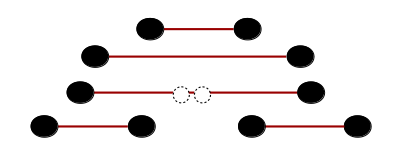
\includegraphics[width=0.9\textwidth]{lundstring.png}
\caption{An illustration of the Lund string model. As the quark/anti-quark pair move further apart, the increase in potential energy creates an additional quark/anti-quark pair.}
\label{fig:lund}
\end{figure}


%The second method, the cluster model, is based on the fact that at any energy scale clusters of color singlet partons appear with an invariant mass distribution that is independant of the starting hadronization energy scale. 

%\qquad In the cluster model, all gluons are forced to split into quark-antiquark pairs following hadronization. This results in a series of color singlet quark-antiquark clusters. Clusters above a given threshold are required to break up until all clusters are below the cutoff value. A probablity is defined for low energy clusters to decay to one hadron. The remaining clusters are treated as excited mesons and are allowed to decay according to flavor and spin considerations. By decaying some clusters to one hadron, the cluster model improves the modeling of hadrons that carry most of the momentum of their parent jets.

\subsection{Monte Carlo Generator Software}\label{mcsoftware}

\qquad A variety of different Monte Carlo generators are used at CMS. {\sc MadGraph} \cite{Alwall:2014hca} is used to compute matrix elements. Next to leading order (NLO) matrix elements can be computed with the aMC@NLO\cite{Alwall:2014hca} version of {\sc MadGraph} or with {\sc Powheg}\cite{Alioli:2010xd} \cite{Frixione:2007vw} \cite{Nason:2004rx}. NLO calculations are vital for accurately depicting physical processes such as W+Jets or Z+Jets. These calculations include quark and gluon loops that complement the fundamental hard scattering process. However, {\sc MadGraph} and {\sc Powheg} do not include parton showering and hadronization, which are necessary for accurate modelling of proton-proton collisions and jet formation, as discussed in section \ref{ppcoll}. The output of the matrix element generators are piped into {\sc Pythia}, which models parton showers and hadronization using the Lund String Model. While {\sc Pythia} is a powerful tool for calculating parton showering and hadronization, it is only a leading order (LO) generator, so it must receive matrix element results {\sc MadGraph} or {\sc Powheg} to give results at the desired degree of precision. After hadronization, some heavy states may still need to decay. The $\tau$ lepton is too short lived to be directly observed in the detector, so any Monte Carlo simulation must decay the $\tau$ further. 
{\sc Tauola} \cite{Was:2011tv} is interfaced with {\sc Pythia} to provide an accurate view of $\tau$ decay by taking into account $\tau$ helicity and polarization. The Monte Carlo for FeMtobarn (MCFM) program \cite{Campbell:1999ah}\cite{Campbell:2011bn}\cite{Campbell:2015qma} is used to calculate the expected cross sections of the Monte Carlo simulation. 

%\subsection{Monte Carlo Samples}\label{mcsamples}
%\subsubsection{LFV Higgs}\label{mclfv}
%\begin{table}[hbtp]
% \begin{center}
% \caption{Monte Carlo simulations used for 8 TeV $H \rightarrow \mu\tau$.}
%  \label{tab:8TeVLFV}
%  \vspace{0.1in}
%  \begin{tabular}{|l|l|l|} \hline
%                                                   & Description &  Generator & $\sigma$(pb)     \\ \hline
%LFV Higgs Signal (GGF)          & Pythia8             &  19.6             \\ \hline
%LFV Higgs Signal (VBF)          & Pythia8             &  1.58             \\ \hline
%SM Higgs Signal (GGF)           & Pythia6+Tauola             &  19.6             \\ \hline
%SM Higgs Signal (VBF)           & Pythia6+Tauola             &  1.58             \\ \hline
%$W \rightarrow l\nu + jets$          & Madgraph + Pythia6             &  37509             \\ \hline
%$qq \rightarrow l^{+}l^{-} + jets$   & Madgraph + Pythia6             &  19.6             \\ \hline
%LFV Higgs Signal (GGF)          & Pythia8             &  19.6             \\ \hline
%LFV Higgs Signal (GGF)          & Pythia8             &  19.6             \\ \hline
%LFV Higgs Signal (GGF)          & Pythia8             &  19.6             \\ \hline

%Selection(lepton1), Selection(lepton2)              & Region I              &  Region II             \\ \hline
%  \end{tabular}
% \end{center}
%\end{table}


\section{Detector Simulation}\label{detectorsim}
\qquad After the simulation of the physical process, complete with parton showering and hadronization, it is necessary to model the interactions of the finale state particles with the CMS detector. This is done using GEANT4\cite{Allison:2006ve}. First, an accurate model of the CMS detector must be built in GEANT4, defining both the geometry and material components of the detector. The simulation is then carried out in two steps: tracking and detector response. The tracking step simulates the passage of particles through matter, modelling the energy lost based on the particles and the detector material. The next step is to model the detector response. This will simulate the signal that each event will create. After the the GEANT4 simulation has completed, the output is converted to the same software format as the actual data and then reconstructed with the same algorithms discussed in section \ref{pflow}. The fully simulated events will retain all of the original Monte Carlo scattering information, so we can now understand what a particular physical process will look like from the point of view of the CMS detector. This allows us to study and improve the reconstruction of proton-proton collisions at CMS.

\chapter{Event Reconstruction}\label{eventreco}

\qquad Studying physical processes requires reconstructing the particles in each event from the detector response. This is accomplished via the particle flow algorithm, which is discussed in section \ref{pflow}. Specific applications to physics objects are discussed in subsequent sections of this chapter. In particular, the important objects for $H \rightarrow \mu\tau$ are muons, electrons, hadronic tau deposits, jets, and missing energy. The important objects for W+Jets are muons, jets, and missing energy.
\section{Particle Flow Overview}\label{pflow}
\qquad As discussed in section \ref{cms}, the CMS detector is divided into many layers, each of which is responsible for measuring a unique part of an event. The detector response from each layer can be thought of as a building block for an event. Particle flow uses a series of algorithms to link these blocks to reconstruct the particles in the event. More specifically, particle flow algorithms link tracks in the tracker to energy deposits in the calorimeters or tracks in the muon system. Energy deposits that have no tracks associated with them are assumed to be due to neutral particles. Ultimately, effective tracking algorithms are necessary before most particles can be identified.

\qquad Tracking algorithms build up the full tracks iteratively. Track construction begins by identifying hits in the pixel layer. There must be hits in at least three pixel layers with an energy of at least 200 MeV ~\cite{Chatrchyan:2014fea} These collections of hits are used to seed a track. The track is then propagated to subsequent layers of the tracker by a Kalman Filter technique ~\cite{Fruhwirth:1987fm}. A $\chi^2$ fit is then used to identify the silicon strip hits that best correspond to the pixel triplets. All hits in the track are then removed from the list of hits to consider, and the algorithm is repeated for subsequent collections of pixel triplets and silicon strip deposits. This is shown in figure ~\ref{fig:iteratetrack}.

\begin{figure}[here]
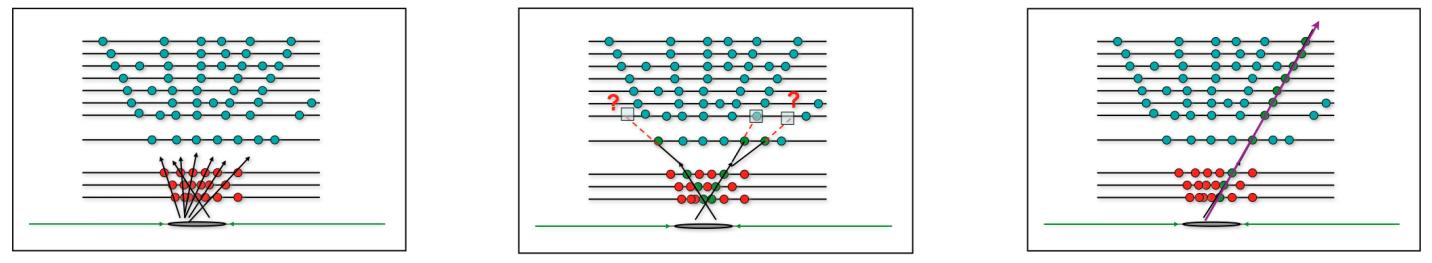
\includegraphics[width=1.1\textwidth]{iterative_tracking.jpg}
\caption{A visual depiction of the iterative tracking algorithm\cite{Tosi:1956757}. First, pixel triplets are identified. Then a $\chi^{2}$ fit is used to determine the best match of pixel hits and tracker hits, ultimately identifying a track. This identified track will then be removed and the algorithm will then find the second best track candidate. }
\label{fig:iteratetrack}
\end{figure}


\qquad Nuclear interactions in the tracker material can cause tracks to appear displaced. These interactions are identified by linking three tracks to a common secondary vertex. A secondary vertex is a vertex that is displaced from the primary vertex of the collision. The primary vertex is identified by selecting the vertex with the highest $p_{T}^{2}$ sum of its associated tracks. A primary track is required to link the secondary vertex to the primary vertex. The tracks linked to the secondary vertex are required to have an invariant mass greater than 200 MeV. These secondary vertices are distinguished from those discussion in section \ref{bjets} by their distance from the beam axis. Identified secondary vertices from b-jets are required to form within $d_{xy} <$ 0.2 cm of the beam axis, but as discussed in section \ref{tracker}, the innermost component of the tracker is located at $d_{xy} =$ 4 cm from the beam axis. 


\qquad After identifying the tracks, their positions are extrapolated to associate them with energy deposits in other parts of the detector. Due to the magnetic field, the radius of the track will depend on the particle's momentum. The momentum of the track is compared to the energy measured in the calorimeters or the muon system to determine if the track was associated with the deposit. In this way, tracks and calorimeter deposits are linked together to reconstruct each particle of the event. Each particle type has its own unique reconstruction conditions, which are described below.

\section{Electrons}\label{electrons}

\qquad Electrons are identified by associating tracks found in the ECAL to objects known as ``superclusters." As electrons interact with the tracker, they will lose kinetic energy in the form of radiated photons. This is known as bremsstrahlung radiation ~\cite{griffiths1999introduction}. These radiated photons are not affected by the magnetic field of CMS. As a result, the electron energy will be spread out in $(\eta,\phi)$ in the ECAL because the radiated photons are unaffected by the magnetic field. 

\qquad Tracks from the standard iterative tracking procedure (section \ref{pflow} are used as electron candidates. Their $p_{T}$ is required to be greater than 2 GeV. The electrons may not interact substantially with the tracker, so if the track is propagated to the ECAL (section \ref{ecal}) and if its $p_{T}$ matches the ECAL cluster deposit, then the track is pre-identified as an electron. Otherwise the track is fit with a Gaussian-sum filter (GSF) to account for the non-Gaussian energy loss~\cite{Adam:815410} in the tracker. A boosted decision tree ~\cite{Hocker:2007ht} is then used to select the final GSF electron track candidates.  

\qquad Photons are neutral particles and will therefore not leave any tracks in the tracker. Bremsstrahlung photons are reconstructed by examining tangents to the tracks at each tracker layer, where the bremsstrahlung radiation may have occurred as the electrons passed through the layer. These tangent tracks are extrapolated to the ECAL. If any of the extrapolated bremsstrahlung photon tracks are associated with clusters in the ECAL then those ECAL clusters are considered part of the electron supercluster. A similar procedure is used to add clusters associated with bremsstrahlung photon $e^{+}e^{-}$ pair production. Tracks associated with the supercluster have a high probability of being associated with jets or other particles. A more sophisticated method is needed to properly associate electron tracks with the supercluster.

\qquad The GSF electron tracks are matched to an ECAL supercluster of at least 10 GeV. No more than 10$\%$ of the ECAL energy should be found in a topologically linked section of the HCAL. A boosted decision tree ~\cite{Hocker:2007ht} takes as inputs the ECAL energy, HCAL energy, GSF track quality, among other parameters, and is trained to identify electrons. If there is no associated GSF track the particle flow candidate is defined as a photon. The reconstruction efficiency for electrons is about 90$\%$ for $p_{T} > 20$ GeV. ~\cite{Khachatryan:2015hwa}

\qquad In the 2012 analyses at $\sqrt{s}$ = 8 TeV, a cut based ID is used \cite{Khachatryan:2015hwa}. The cuts used differ between the calorimeter barrel ($|\eta| < 1.479$) and the endcap ($1.479 < |\eta| < 2.5$). In the barrel, the extension of the shower in the $\eta$ direction ($\sigma_{\eta\eta}$) is required to be less than 0.01. The ratio of the energy deposits ($H/E$) between the HCAL (section \ref{hcal}) and the ECAL (section \ref{ecal}) must be less than 0.12.    The distances from the vertex, $d_{0}$ and $d_{Z}$ (section \ref{cms}) must be less than 0.02 cm and 0.2 cm respectively. The supercluster energy $E_{SC}$ and the track momentum at the closest point to the vertex ($p$) are also used as discriminators, with the requirement that $1/E_{SC} - 1/p < 0.05$. In the endcap the $\sigma_{\eta\eta}$ cut is loosened to 0.03 and the $H/E$ cut is tightened to 0.10.

\qquad In the 2015 analyses at $\sqrt{s}$ = 13 TeV, a boosted decision tree is used to optimize the electron selection. MVA discriminators are used to require an electron efficiency of 90\%.

\qquad Electrons are required to be isolated from additional particles in the event. The $p_{T}$ of charged hadrons, neutral hadrons, and photons is summed within a cone of radius $\Delta R < 0.3$ around the electron.  Pileup corrections are applied for additional particles not associated with the primary vertex. The particle flow isolation is defined as $I_{PF}^{e} = \left(\sum\limits^{Ch. had} p_{T} + max(0, \sum\limits^{N. had.} p_{T} + \sum\limits^{\gamma} p_{T} - 0.5 \sum\limits^{PU} p_{T}\right)/p_{T}^{e}$. The factor of 0.5 corresponds to an approximate average ratio of neutral to charged particles, as measured in jets \cite{CMS-PAS-PFT-10-002}. Alternatively, the effective area method can be used to estimate the pileup. The contribution from the pileup, $p_{T}^{PU}$, is defined as $p_{T}^{PU} = \rho A_{eff}$. Here $\rho$ is the average energy density in the event, defined as the median of the energy density distribution for particles within the area of any jet (section \ref{jets}) in the event.\cite{Khachatryan:2015hwa} {\sc Fastjet} \cite{Cacciari:2011ma} is used to determine $A_{eff}$, the effective area of of the clustered jet.  


\section{Muons}\label{muons}
\qquad Muons are highly penetrating particles~\cite{Agashe:2014kda} that deposit a minimal amount of energy in the ECAL and HCAL before depositing the remainder of their energies in the muon system. The muon system is discussed further in section \ref{muonsys}. 

\qquad Muons are identified in three different ways. Standalone muons are identified based on hits in the DT, CSC, and RPC elements of the muon system. Hits in the DT's and CSC's are used as a seeds for a Kalman Filter (section \ref{pflow}) fit of the DT, CSC, and RPC hits. The resulting track is defined as a standalone muon.~\cite{Chatrchyan:2013sba} If a standalone muon track is matched to a tracker track, then the two tracks are combined using the Kalman Filter technique to identify a global muon. 

\qquad Tracker muons are constructed by extrapolating all tracker tracks with $p_{T} > 0.5$ GeV and $p > 2.5$ GeV to the muon system. If the track matches a small segment of DT and CSC hits, the track is considered to be a tracker muon. Tracker muons improve efficiency for muons with low $p_{T} < 5$ GeV because low energy muons won't register enough hits in the muon system to be identified as standalone or global muons. However, at high $p_{T} > 200$ GeV, the momentum resolution of the muon system outperforms the momentum resolution of the tracker.

\qquad The muon algorithms are very efficient, with approximately 99$\%$ of muons successfully identified in the tracker or the muon system.~\cite{Chatrchyan:2013sba} To reduce the fake rate due to hadrons punching through the calorimeters, global muons are required to be isolated, with no more than 10$\%$ of their energy measured by the calorimeters or the tracker inside a cone of $\Delta R < 0.3$. Additionally, charged hadrons may be reclassified as muons if their is a large discrepancy between their track $p_{T}$ and the sum of their particle flow linked calorimeter deposits. 

\qquad Additional tight identification criteria are applied to muons used in the analyses in sections \ref{lfv} and \ref{wjets}. Global muons are required to be within $d_{xy} <$ 0.2 cm and $d_{z} <$ 0.5 cm of the primary vertex. Muons are required to have recorded at least one hit in the pixel system (section \ref{tracker}) and hits in at least six tracker layers. A particle flow based isolation requirement is defined for muons, analogous to the definition for electrons in section \ref{electrons}. 
$I_{PF}^{\mu} = \left(\sum\limits^{Ch. had} p_{T} + max(0, \sum\limits^{N. had.} p_{T} + \sum\limits^{e,\gamma} p_{T} - 0.5 \sum\limits^{PU} p_{T}\right)/p_{T}^{\mu}$. The isolation is computed in a radius of $\Delta R < 0.4$. 


\section{Hadrons}\label{hadrons}
Hadrons are identified after the unique signatures of electrons, photons, and muons are already identified and removed from the list of remaining particle flow candidates. Neutral hadrons will only deposit energy in the calorimeters, while charged hadrons have associated tracks. For charged hadrons, the uncertainty in $p_{T}$ returned by the track fit must be smaller than the calorimeter energy resolution for charged hadrons, described in sections \ref{ecal} and \ref{hcal}. The hadronic deposits are used to reconstruct jets and hadronic tau decays.

\subsection{Jets}\label{jets}
\qquad After hadronic deposits are reconstructed via particle flow, the anti-$k_{t}$ ~\cite{Cacciari:2008gp} algorithm is used to cluster the deposits and define jets. A distance metric between hadronic particles $i$ and $j$ is defined: $d_{ij} = min(\frac{1}{k_{ti}^{2}},\frac{1}{k_{tj}^{2}})\frac{\Delta_{ij}^{2}}{R^{2}}$. Here $k_{t}$ is the transverse momentum and $\Delta_{ij}^{2} = (y_{i}-y_{j})^{2} + (\phi_{i} - \phi_{j})$, where $y$ and $\phi$ are the rapidity and azimuth of the particle, as defined in section \ref{cms}. At CMS, a radius of $R = 0.5 (0.4)$ is used at 8 TeV (13 TeV). The radius is chosen to minimize the effect of pileup on the energy of the clustered jet. The distance between particle $i$ and the beam is defined as $d_{iB} = \frac{1}{k_{ti}^{2}}$.

\qquad Beginning from a particle $j$, neighboring particles $i$ are combined while $d_{ij} < d_{ib}$. Otherwise, $i$ is considered the seed for a different jet. The results of this algorithm are show in Figure ~\ref{fig:antikt}. The anti-$k_{t}$ algorithm is infra-red safe and collinear safe~\cite{Cacciari:2008gp} which means that the jet clustering process is not affected significantly by low energy soft radiation. The anti-$k_{t}$ algorithm is applied to jets at CMS via the {\sc Fastjet} framework\cite{Cacciari:2011ma}.

\begin{figure}[here]
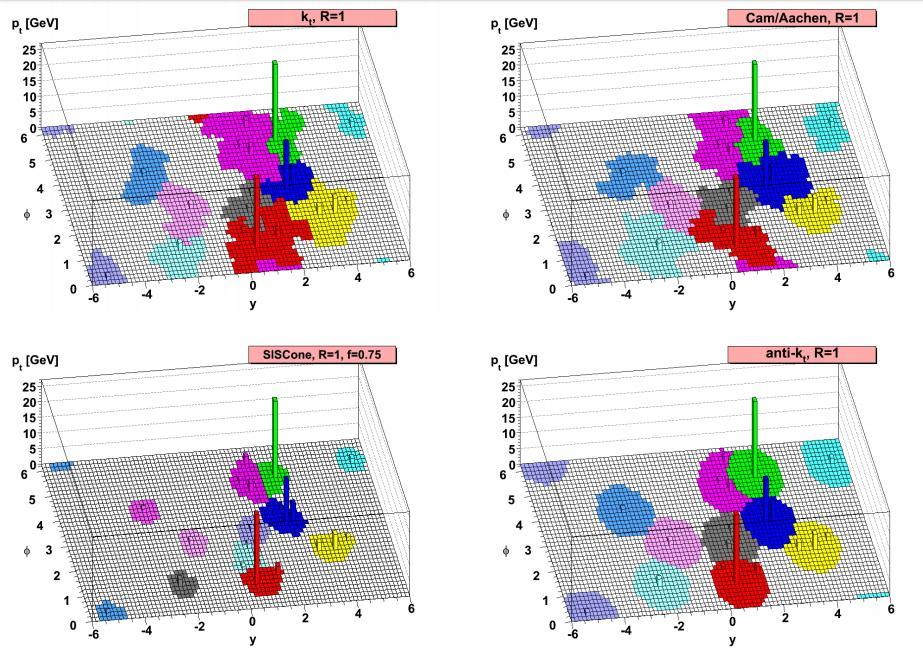
\includegraphics[width=0.9\textwidth]{antikt.jpg}
\caption{Performance of the anti-$k_{t}$ algorithm.~\cite{Cacciari:2008gp} Note that the anti-$k_{t}$ algorithm is the only algorithm that generates a circular hard jet. }
\label{fig:antikt}
\end{figure}

\qquad Charged hadron subtraction is used to reduce the dependence of the jets on pileup (section \ref{ppcoll}) The majority of jet energy is carried by charged hadrons. For example, at $p_{T} = 100$ GeV charged hadrons are responsible for 65$\%$ of the jet energy. Photons carry 25$\%$ of the energy and neutral hadrons carry 10$\%$ of the energy. The charged hadron constituents of the jets still have track information stored via the particle flow algorithm. Any charged hadrons associated with pileup vertices instead of the primary vertex are retroactively removed from the jet.~\cite{Kirschenmann:1627818}

\qquad Multiple types of corrections are applied to the jets. First, the average $p_{T}$ density per unit area is used to estimate the soft jet activity, which is associated with a combination of the underlying event, electronic noise, and pileup ~\cite{Kirschenmann:1627818}. This energy is subtracted using $\eta$ and $p_{T}$ dependant scale factors. The next level of corrections use Monte Carlo to calibrate the differences between reconstructed jets and generated jets in bins of $p_{T}$ and $\eta$. This step is designed to account for detector imperfections, such as a non-linear $p_{T}$ response of the calorimeters or variations in response with respect to $\eta$. Finally, data-driven residual scale factors are computed by measuring jet $p_{T}$ imbalances in dijet events and Z/$\gamma$+jets.

\qquad Jets which originate from pileup rather than the hard scattering process of interest are identified and removed. A boosted decision tree is trained using a Z+jets Monte Carlo sample produced with {\sc MadGraph} and {\sc Pythia}. Jet shower shape and vertex related variables are used as inputs to identify reconstructed jets which are not matched to a generator level hard scattering process\cite{CMS-PAS-JME-13-005}.

\subsubsection{B-Jets}\label{bjets}
\qquad Jets which originate from b quark decays are referred to as b-jets. B quarks produced in the hard scattering event can travel a measurable distance before decaying. B-jets are identified by finding jets which originate from a secondary vertex, displaced in $d_{xy}$ from the primary vertex. Secondary vertices are required to share less than 65\% of their associated tracks with the primary vertex and have at least a 3$\sigma$ radial distance significance from the primary vertex. The secondary vertices must be within $d_{xy} <$0.2 cm and $d_{z} <$17 cm of the primary vertex, which accounts for the time it takes the b quark to hadronize. The tracks from the secondary vertices must have $p_{T} >$ 1 GeV and have at least eight associated hits in the tracker. Tracks that pass these requirements are used as inputs in the Combined Secondary Vertex (CSV) algorithm. This algorithm identifies b-jets using vertex and tracker related variables to identify b-jets and is trained with a $t\bar{t}$ sample. The b-tagging efficiency is 85\%. \cite{Chatrchyan:2012jua}

\subsection{Taus}\label{taus}

\qquad As discussed in section \ref{elemforces}, taus can decay leptonically to electrons or muons, or hadronically to quarks. Taus are identified separately depending on their decay products, so the identification of leptonic tau decays has already been discussed in sections \ref{muons} and \ref{hadrons}, which describe the identification of electrons and muons respectively. This section will discuss the identification of hadronic taus. As discussed in section \ref{elemforces}, taus can decay hadronically in three dominant ways: To a charged pion, to a charged pion and a neutral pion, or to three pions. These decays have branching fractions of 11.6\%, 26.0\%, and 9.8\%, respectively.

\qquad If the tau decays exclusively to charged hadrons, the hadronic tau ($\tau_{h}$) is identified by comparing the invariant mass of the hadrons to the invariant mass of the tau. For example, if the tau decays to three charged pions, the invariant mass of the decay products must be between 0.8 GeV and 1.5 GeV, and the tracks must originate within $\Delta z < 0.4$ cm of the same event vertex ~\cite{1748-0221-7-01-P01001}, where $\Delta z$ is the distance in the x-y plane of CMS, as discussed in section \ref{cms}. Mass windows of 50-200 MeV and 0.3-1.3 GeV are used for charged pion decays and charged pion plus neutral pion decays, respectively. 

\qquad If a neutral pion is involved in the hadronic tau decay, then the hadron plus strips (HPS) method must be used to identify the taus. Neutral pions convert to energetic photons in the tracker which then produce electron positron pairs. These particles will be bent in opposite directions in the magnetic field of CMS and will deposit their energy in the ECAL in a strip in $\phi$. The maximal distance between hadronic tau candidates and strips is $\Delta R = 3.0/p_{T}^{\tau}$. The strip sizes are 0.05 $\times$ 0.20 in the ($\eta$,$\phi$) plane. The size is elongated in $\phi$ because the $e^{+}e^{-}$ pair will be bent in $\phi$ due to the magnetic field. In 13 TeV, the strip sizes are allowed to vary in a dynamic way that depends on the $p_{T}$ weighted average of all $e/ \gamma$ objects in the strip. The strip size is allowed to vary from (0.05,0.05) to (0.15,0.30) in the ($\eta$,$\phi$) plane.If a charged hadron from particle flow is linked to a strip in ECAL, and the invariant mass of the system is compatible with the hadronic tau mass, then the object is identified as a tau. The probability to reconstruct the tau decay mode is 80\%, as measured in $Z \rightarrow \tau\tau$ events.

\qquad The particle flow tau isolation, $I_{PF}^{\tau}$, is computed by summing momenta of particle flow candidates within a cone of $\Delta R$ = 0.5 (0.4 at 13 TeV) around the tau. $I_{PF}^{\tau} =  \sum\limits^{Ch. had} p_{T} + \sum\limits^{N. had.} p_{T} + \sum\limits^{\gamma} p_{T} - 0.4576 \sum\limits^{PU} p_{T}$ The 0.4576 factor is chosen to make the ID independent of pileup. The tight working point requires $I_{PF}^{\tau} <$ 0.8 GeV and has an ID efficiency of 50 \% in 8 TeV data. \cite{CMS-DP-2014-015}

\section{Missing Energy} \label{met}
\qquad There are some particles, for example neutrinos or dark matter candidates, that CMS cannot detect. They can be measured by applying the principle of conservation of momentum. The transverse vector sum of all particle flow candidates in the event is computed. If CMS detected every particle, this sum would be zero. Therefore, the energy that CMS did not detect can be quantified by reversing the vector sum of the particles that were detected. If the jet energy corrections are included in the vector sum, the transverse missing energy (MET) is said to be Type 1 corrected ~\cite{Khachatryan:2014gga}

\chapter{Lepton Flavor Violating Decays of the Higgs Boson}\label{lfv}

\section{Analysis Overview}\label{lfvoverview}
\qquad A search for a lepton flavor violating (LFV) decay of a Higgs boson is performed in two channels: $H \rightarrow \mu\tau_{e}$ and $H \rightarrow \mu\tau_{h}$, where $\tau_{h}$ and $\tau_{e}$ are taus reconstructed in the hadronic and electronic decay channels respectively. As mentioned in section \ref{higgspheno}, these channels have a similar signature as the Standard Model $H \rightarrow \tau_{\mu} \tau_{h}$ and $H \rightarrow \tau_{\mu}\tau_{e}$ searches, with a significant kinematic difference due to the muon arising directly from the Higgs decay. All the neutrinos in the event will arise from the tau decay. Because the tau is heavily boosted, the neutrinos will be collinear with the visible tau decay products. The term ``visible decay products" is used to denote the tau decay products that CMS can detect directly, which are electrons, muons, and hadrons. Neutrinos register as missing transverse energy in the event and are detected indirectly as discussed in section \ref{met}. The missing transverse energy in the event is the sum of the energy of all unidentified particles, so the individual neutrino momenta cannot be measured directly. In order to calculate the invariant mass (section \ref{kindef}) of the final state objects the collinear approximation must be used.

\qquad The collinear approximation\cite{Ellis:1987xu} arises from the observation that since the mass of the Higgs is much greater than the mass of the tau, the tau decay products are highly boosted in the direction of the original tau. Therefore, the neutrino momentum can be approximated to be in the same direction as the other visible decay products of the tau. The component of the missing transverse energy in the direction of the visible tau decay products is used to estimate the transverse component of the neutrino momentum:

\begin{equation}
\vec{p}_{T}^{\nu} = \vec{E}_{T}^{miss} \dot \hat{p}_{T}^{\tau_{vis}}
\end{equation}

The fraction of the tau momentum carried by the visible tau decay products, $x_{\tau_{vis}}$, is given by:

\begin{equation}
x_{\tau_{vis}} = \frac{|\vec{p}_{T}^{\tau_{vis}}|}{|\vec{p}_{T}^{\tau_{vis}}| + |\vec{p}_{T}^{\nu}|}
\end{equation}

The tau four momentum is then $\frac{1}{x_{\tau_{vis}}}\left(|\vec{p}^{\tau_{vis}}|,\vec{p}^{\tau_{vis}}\right)$. The mass of the Higgs boson is much greater than the mass of the tau or muon or electron, so the approximation $M_{H} \gg m_{\tau}^2,m_{l}^2$ is valid. This yields the collinear mass equation:

\begin{equation} 
M_{H} = M_{collinear} = \frac{M_{vis}}{\sqrt{x_{\tau_{vis}}}}
\end{equation}

The Higgs mass has now been defined in terms of the mass of the visible decay products, which can be directly measured by CMS. As shown in figure \ref{fig:MvisMcol} the collinear mass gives an improved mass resolution over the visible mass, in addition to peaking at the expected value of 125 GeV. 

\begin{figure*}[hbtp]\begin{center}
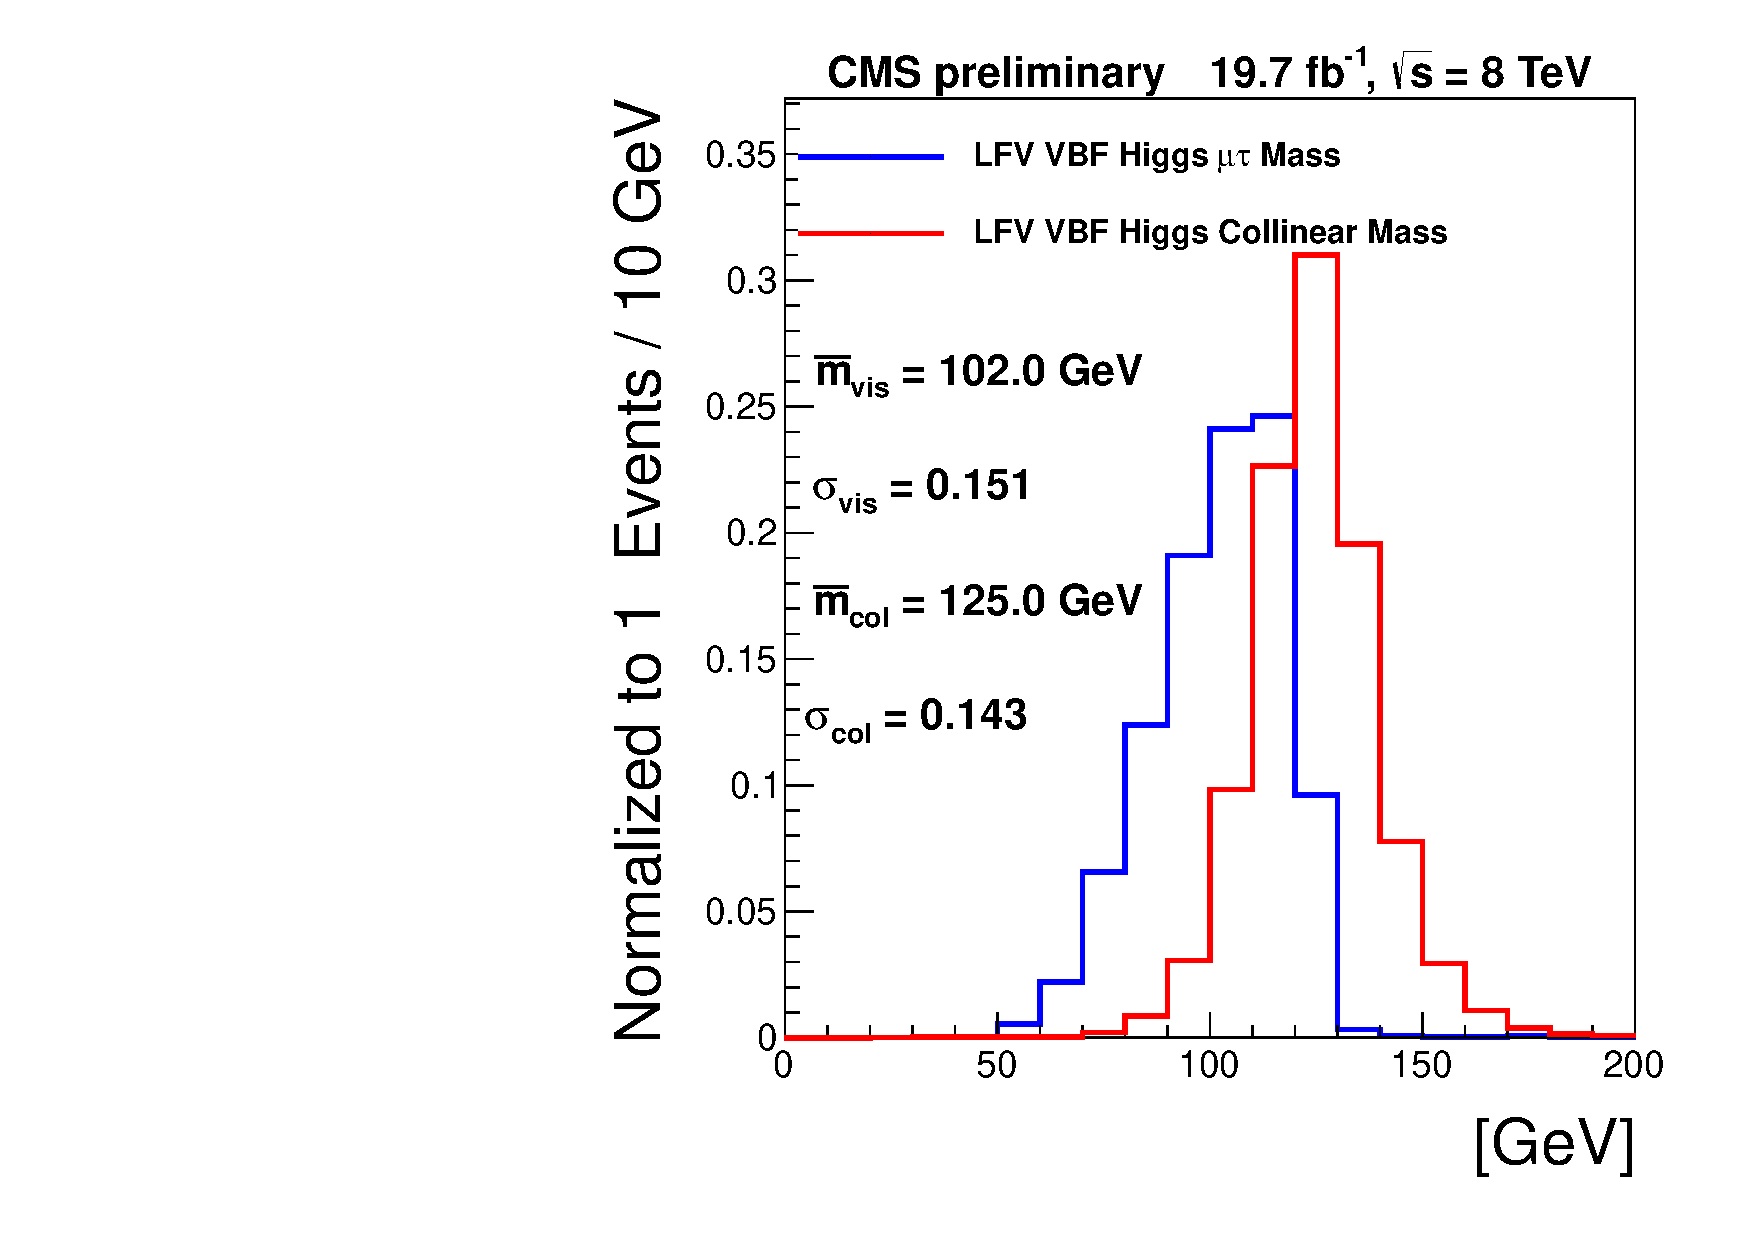
\includegraphics[height=5.5cm]{masses_muhad_VBF_After_Presel_signal.pdf}
 \caption{$M_{vis}$  and $M_{collinear}$  shape comparisons after the pre-selection for the $H \rightarrow \mu\tau_{h}$ channel}
 \label{fig:MvisMcol}\end{center}\end{figure*}
 
\section{Misidentified Leptons}\label{fakes}
\qquad Jets may be mistakenly identified as leptons. These misidentified leptons are referred to as ``fakes." Misidentified leptons are produced by jets in W+Jets and QCD multi-jet events. The W+Jets background is particularly significant as the largest irreducible background in this analysis. If a jet is misidentified as a tau and the W boson decays muonically, then the kinematics of the event may be identical to the LFV signal: a muon, a tau, and missing energy opposite to the muon. 

\qquad This background is estimated using a data driven method. The same preselection cuts are used, but the isolation of one of the leptons is inverted, so that is it surrounded by other PF objects in the event. This enriches the contributions from W+jets and QCD multijet events and gives a larger sample of data statistics for estimating the background. 
The probability for particle flow objects to be misidentified as leptons is measured in an independent collision data set of $Z \rightarrow \mu\mu + X$, where $X$ is the lepton whose misidentification rate is being measured. The $Z \rightarrow \mu\mu + X$ sample is selected by applying the loose preselection cuts described in section \ref{eventsel} to a final state of two muons plus an addition electron, muon, or tau corresponding to the leptonic fake rate that is being measured. The two muons are required to have opposite sign, and the sign of the additional lepton is not specified. The two muons are also required to have an invariant mass between 75 GeV and 105 GeV.

\qquad The misidentification probability is applied to a data sample rich in misidentified leptons to compute the misidentified lepton background in the signal sample. This technique is shown schematically in Table 4 in which four regions are defined. Region I is defined by the preselection cuts described in section \ref{eventsel}. Region III has the same selections as Region I but with a nonisolated requirement on the lepton whose fake rate is being measured. This requirement varies for each lepton and is described in more detail below. Regions I and III are the signal and background enriched regions, respectively, and Regions II and IV are the control regions, with the same selections as Regions I and III but with a same sign lepton requirement. The control regions are designed to maximize the number of fake lepton events while minimizing other backgrounds in order to directly test the accuracy of the fake rate method. This technique is illustrated in Table \ref{tab:fakeratediagram}. 

\begin{table}[hbt]
 \centering
 
 \renewcommand{\arraystretch}{1.1}
 \caption{Definition of the regions used to estimate the misidentified lepton background. The different regions have different requirements for the
isolation and the relative charge of the two leptons $\ell^{\pm}_{1}$ and $\ell^{\pm}_{2}$, which can be $e$, $\mu$ or $\tau_{h}$.}
  \label{tab:fakeratediagram}
  
  \begin{tabular}{c|c}  
  Opposite-sign leptons & Same-sign leptons \\
  \hline
% \rule[-5pt]{0pt}{20pt}
\textbf{Region I}              &  \textbf{Region II}             \\ \hline
$\ell^{\pm}_{1}$(isolated)  &  $\ell^{\pm}_{1}$(isolated)             \\
$\ell^{\mp}_{2}$(isolated)  &  $\ell^{\pm}_{2}$(isolated)             \\

\hline \hline
% \rule[-5pt]{0pt}{20pt}
\textbf{Region III}           &  \textbf{Region IV}             \\ \hline
$\ell^{\pm}_{1}$(isolated)  &  $\ell^{\pm}_{1}$(isolated)             \\
$\ell^{\mp}_{2}$(non-isolated )  &  $\ell^{\pm}_{2}$(non-isolated)             \\
\hline
  \end{tabular}
  
\end{table}
\subsection{Misidentified Taus}\label{misidtaus}
\qquad In the $H \rightarrow \mu\tau_{h}$ channel, the $\tau_{h}$ candidate can arise from a misidentified jet coming predominantly from W+jets and QCD multijet events. The misidentification rate $f_{\tau_{h}}$ is measured in $Z \rightarrow \mu\mu +X$ events selected in data, where $X$ is an object identified as a $\tau_{h}$ candidate that passes the loose isolation requirement of $I_{PF}^{\tau} <$ 2 GeV (see section \ref{taus} for a definition of $I_{PF}^{\tau}$). The factor $f_{\tau_{h}}$ is defined as the fraction of these loosely isolated $\tau_{h}$ candidates that pass the tighter isolation requirement, $I_{PF}^{\tau} <$ 0.8 GeV, used to define the signal region. The misidentification rate measured in $Z\rightarrow \mu\mu+X$ collision data is compared to the measured rate in simulation and is found to be in agreement, as shown in figures \ref{fig:taufakerate8TeV} and \ref{fig:taufakerate13TeV}.

\begin{figure*}[hbtp]\centering
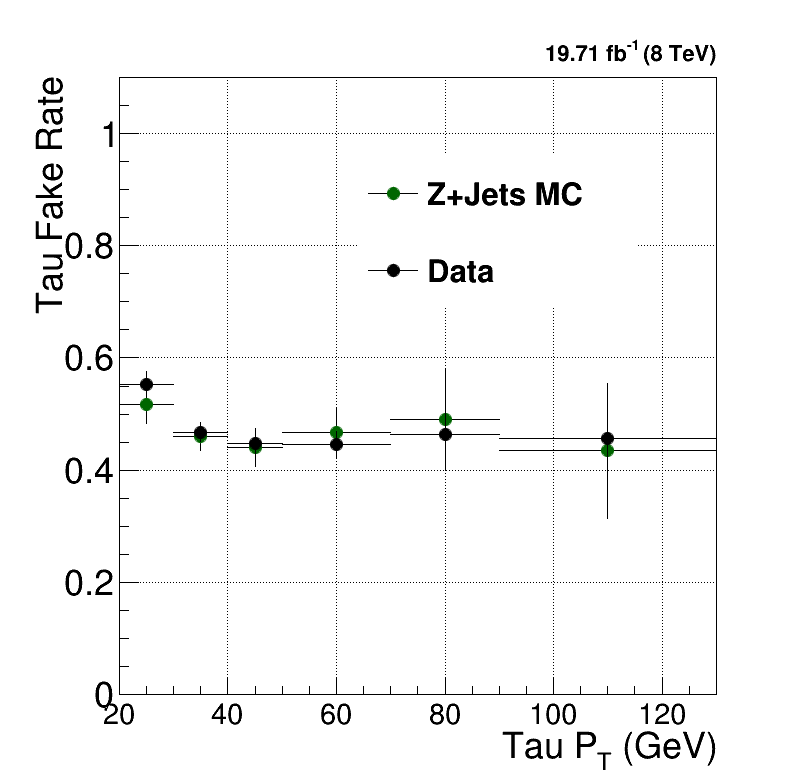
\includegraphics[width=0.48\textwidth]{tightOldIso_looseOldIso_tPt_fakeRate_8TeV.png}
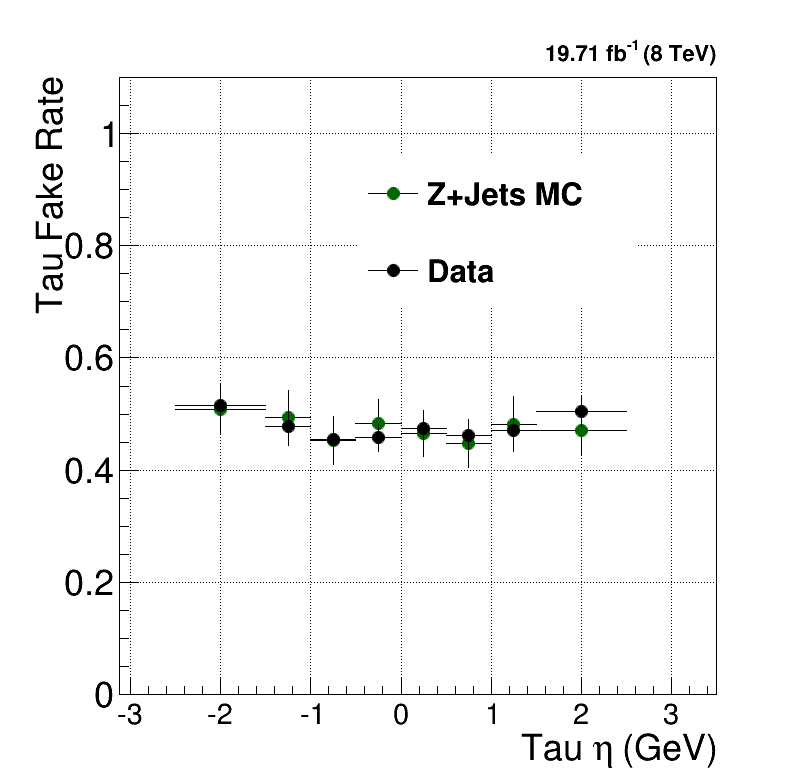
\includegraphics[width=0.48\textwidth]{tightOldIso_looseOldIso_tEta_fakeRate_8TeV.png}
\caption{Distributions of $f_{tau_{h}}$ as a function of $ p_{T}^{\tau}$ (left) and $\eta^{\tau}$ (right) in $\sqrt{s}$ = 8 TeV.}
\label{fig:taufakerate8TeV}\end{figure*}

\begin{figure*}[hbtp]\centering
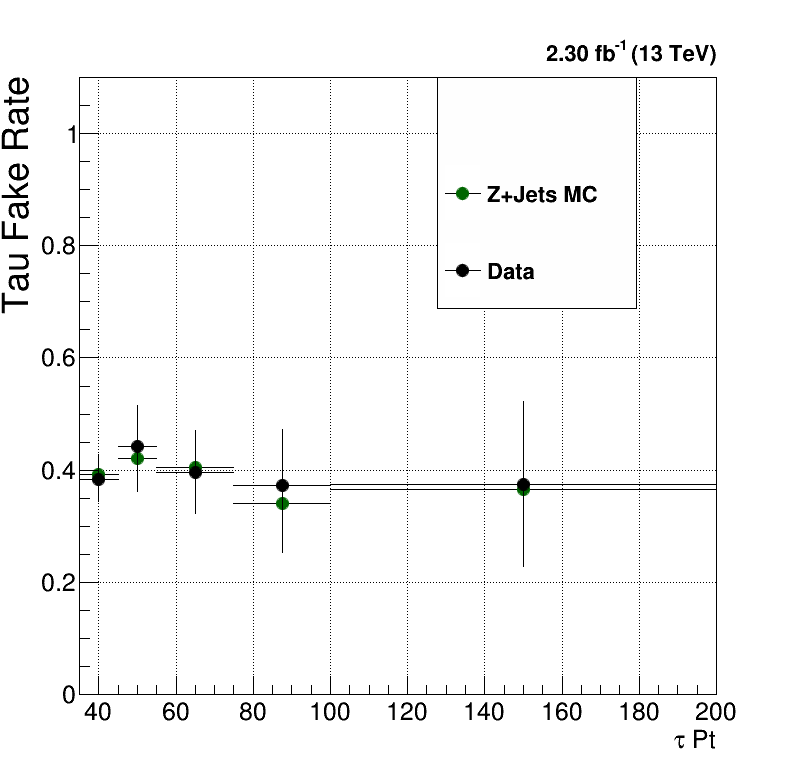
\includegraphics[width=0.48\textwidth]{tightOldIso_looseOldIso_tPt_fakeRate_13TeV.png}
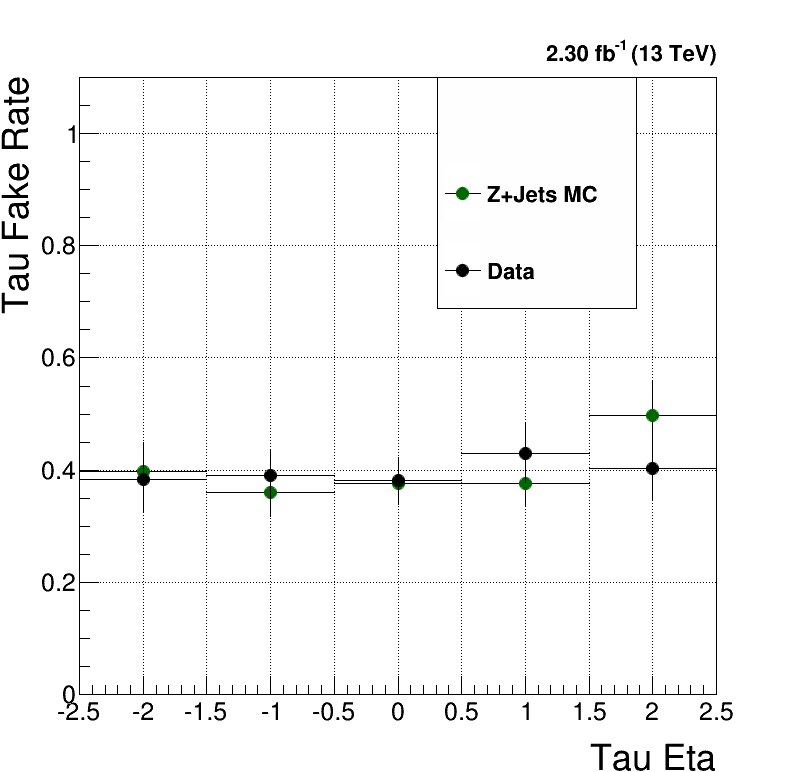
\includegraphics[width=0.48\textwidth]{tightOldIso_looseOldIso_tEta_fakeRate_13TeV.png}
\caption{Distributions of $f_{tau_{h}}$ as a function of $ p_{T}^{\tau}$ (left) and $\eta^{\tau}$ (right) in $\sqrt{s}$ = 13 TeV.}
\label{fig:taufakerate13TeV}\end{figure*}


\qquad The enriched background regions (III and IV) are defined by requiring the presence of $\tau_{h}$ candidates that pass the looser isolation requirement ($I_{PF}^{\tau} <$ 2 GeV), but do not pass the tight isolation requirement ($I_{PF}^{\tau} <$ 0.8 GeV). The misidentified background yield in the signal region (Region I) is estimated by multiplying the event yield in Region III by a factor $\frac{f_{\tau_{h}}}{1-f_{\tau_{h}}}$. The fake rate factors, which are computed as a function of the tau decay mode, are given in tables \ref{tab:taufakerate8TeV} and \ref{tab:taufakerate13TeV}. The procedure is validated with same-sign $\mu\tau_{h}$ events in Region II by scaling the yield in Region IV by the measured misidentification rates. The control region (Region II) for the $H \rightarrow \mu\tau_{h}$ channel is shown in Figure \ref{fig:samesign_fakes}.

\begin{table}[htbp]
  \centering
  \begin{tabular}{ | l | c |}
    \hline
    Decay Mode & $f_{\tau_{h}}$ \\ \hline \hline
    $\tau \rightarrow \pi^{+}_{ - }$ & 0.53 \\ \hline
    $\tau \rightarrow \pi^{+}_{ - }\pi^{0}$ & 0.48 \\ \hline
    $\tau \rightarrow \pi^{+}_{ - }\pi\pi\pi$& 0.46 \\ \hline
    
  \end{tabular}
  \caption{Measured fake rates $f_{\tau_{h}}$ in 8 TeV data.}
  \label{tab:taufakerate8TeV}
\end{table}

\begin{table}[htbp]
  \centering
  \begin{tabular}{ | l | c | c |}
    \hline
    Decay Mode & $f_{\tau_{h}}$ $\left(|\eta^{\tau}|<1.5\right)$ & $f_{\tau_{h}}$ $\left(|\eta^{\tau}|>1.5\right)$ \\ \hline \hline
    $\tau \rightarrow \pi^{+}_{ - }$ & 0.39 & 0.41 \\ \hline
    $\tau \rightarrow \pi^{+}_{ - }\pi^{0}$ & 0.43 & 0.45 \\ \hline
    $\tau \rightarrow \pi^{+}_{ - }\pi\pi\pi$& 0.36 & 0.35 \\ \hline
  \end{tabular}
  \caption{Measured fake rates $f_{\tau_{h}}$ in 13 TeV data. At 13 TeV a small $\eta$ dependence in $f_{\tau_{h}}$ with respect to the decay mode was observed and $f_{\tau_{h}}$ was computed as a function of $|\eta|$ in two bins}
  \label{tab:taufakerate13TeV}
\end{table}


\subsection{Misidentified Muons and Electrons}
\qquad In the $H \rightarrow \mu\tau_{e}$ channel, Region I is defined by the preselection requirements (section \ref{eventsel}) in in which an isolated muon and an isolated electron are required. At 8 TeV Region III has the same cuts are applied, with the exception that one of the leptons is required to be non-isolated by inverting its isolation selection. This means requiring $I_{PF}^{e} > 0.12$ for the electron fake rate calculation and $I_{PF}^{\mu} > 0.12$ for the muon fake rate calculation. At 13 TeV Region III is constructed in an analogous way as Region III for hadronic taus (section \ref{misidtaus}) by requiring leptons to pass a loose selection but not a tight selection. For the misidentified muon background calculation muons are required to have $0.15 < I_{PF}^{\mu} < 0.25$ and electrons are required to have $I_{PF}^{e}<0.10$. For the misidentified electron background calculation electrons are required to have  $0.10 < I_{PF}^{e} < 0.5$ and muons are required to have $I_{PF}^{\mu} < 0.15$. There are a negligible number of signal events in Region III. Regions II and IV are defined using the same selection criteria as Region I and III, respectively, but same-sign leptons are required instead of opposite sign leptons. The sample in region III is dominated by W+jets and QCD multijet events. The misidentified electron background in Region I is estimated by multiplying the event yield in Region III by a factor $f_{e}$, where $f_{e}$ is the ratio of loosely-isolated to tightly isolated electrons. It is computed in an independent data sample $Z \rightarrow \mu\mu + X$, which $X$ is a particle flow object identified as an electron. At 8 TeV, $f_{e}$ was computed as a continuous function of $p_{T}^{e}$ and $\eta^{e}$. For 13 TeV, a more discrete binning was adopted, and the fake rates $f_{e}$ are shown in table \ref{tab:efakerate13TeV}. Background sources of real leptons, such as diboson events, are subtracted from the $Z \rightarrow \mu\mu +X$ sample, using Monte Carlo simulation to estimate the diboson backgrounds (section \ref{addback}). The misidentified muon background is computed in the same way. In 13 TeV, the muon fake rate has no $p_{T}$ or $\eta$ dependence and is measured to be 0.6. The fake rate method is validated using the same-sign data from regions II and IV. In Figure \ref{fig:samesign_fakes} the observed data yield in Region II is compared to the estimate obtained by scaling the Region IV sample by the measured misidentification rates.

\begin{table}[htbp]
  \centering
  \begin{tabular}{ | l | c | c |}
    \hline
     & $f_{e}$ $\left(|\eta^{e}|<1.45\right)$ & $f_{e}$ $\left(|\eta^{e}|>1.45\right)$ \\ \hline \hline
    $p_{T}^{e} < 15$ & 0.44 & 0.44 \\ \hline
    $15< p_{T}^{e} < 20$& 0.30 & 0.42 \\ \hline
    $20< p_{T}^{e}$    & 0.28 & 0.42 \\ \hline

  \end{tabular}
  \caption{Measured fake rates $f_{e}$ in 13 TeV data, computed in bins of $p_{T}$ and $\eta$.}
  \label{tab:efakerate13TeV}
\end{table}


\begin{figure*}[hbtp]\centering
\includegraphics[width=0.48\textwidth]{/home/aaron/root/hlfv/fakesEle_log.pdf}
\includegraphics[width=0.48\textwidth]{/home/aaron/root/hlfv/fakes_log.pdf}
\caption{Distributions of $M_\text{col}$ for region II compared to the estimate
from scaling the region IV sample by the measured misidentification rates at $\sqrt{s}$ = 8 TeV. The bottom panel in each plot shows the fractional difference between the observed data and the estimate. Left:  $H \rightarrow \mu \tau_{e}$. Right: $H \rightarrow \mu \tau_{h}$. }
\label{fig:samesign_fakes}\end{figure*}


\section{8 TeV Backgrounds and Datasets}
\subsection{Data}
\qquad The search is performed on the 2012, $\sqrt{s}$ = 8 TeV dataset, comprising 19.7$fb^{-1}$ of data. The $H \rightarrow \mu\tau_{h}$ channel selection requires an isolated single muon trigger with a $p_{T}^{\mu}$ threshold of 24 GeV in the range $|\eta| < 2.1$, while the $H \rightarrow \mu\tau_{e}$ channel requires a muon-electron trigger with $p_{T}$ threshold of 17 GeV ($|\eta| < 2.5$) and 8 GeV ($|\eta| < 2.4$), respectively. 
\subsection{LFV Higgs and SM Higgs}
\qquad The signal decay $H \rightarrow \mu\tau$ is implemented via {\sc Pythia}8 \cite{Sjostrand:2014zea}. {\sc Pythia}8 contains decay mechanisms that account for tau polarization and spin, and the interface with {\sc Tauola}\cite{Was:2011tv} is not needed\cite{Sjostrand:2014zea}. The Standard Model $H \rightarrow \tau\tau$ background is modelled using {\sc Powheg}1.0\cite{Frixione:2007nu} and {\sc Tauola}. In addition to the generators, the full GEANT detector simulation is used for each Monte Carlo sample.

%\qquad The largest Monte Carlo backgrounds, such as $Z \rightarrow \tau\tau$ and W+jets, are estimated using data and the smaller backgrounds are estimated with simulation. 
\subsection{Z to tau tau}
\qquad The $Z \rightarrow \tau\tau$ background is estimated using a particle flow embedding technique\cite{CMS-PAS-HIG-12-018}. A sample of $Z \rightarrow \mu\mu$ events is taken from data. The muons are then replaced with simulated tau decays reconstructed with the particle flow algorithm. The key features of the event topology, such as the jets, missing energy, and underlying event, are taken directly from data. Only the tau decays are simulated. The sample is normalized in accordance with the Monte Carlo expectation, using Drell Yan events generated with {\sc MadGraph}\cite{Alwall:2011uj} and {\sc Pythia}6\cite{Sjostrand:2006za}.

\subsection{Additional Backgrounds}\label{addback}
\qquad The remaining backgrounds play a small role in the analysis and are all estimated with simulation. MADGRAPH5, PYTHIA6, and Tauola (section \ref{mcsoftware}) are used to simulate diboson events and events with one top quark and one antitop quark ($t\bar{t}$ events). POWHEG 1.0 (section \ref{mcsoftware}), PYTHIA6, and Tauola are used to simulated single top quark events.

\section{13 TeV Backgrounds and Datasets}

\qquad The search is performed on the 2015, $\sqrt{s}$ = 13 TeV dataset, comprising 2.3$fb^{-1}$ of data. The trigger selection requires an isolated single muon with $p_{T} >$ 20 GeV in the range $|\eta| < 2.4$.

\qquad The LFV and SM Higgs boson samples are generated using {\sc Powheg} 1.0, with CT10 parton distribution functions \cite{Guzzi:2011sv}, interfaced to {\sc Pythia} 8.212\cite{Sjostrand:2014zea}. The {\sc MadGraph} 5.1.3.30 \cite{Alwall:2011uj} generator is used for Z+jets, $t\bar{t}$, and diboson production. {\sc Powheg} is used for single top production. The {\sc Powheg} and {\sc MadGraph} generators are interfaced to {\sc Pythia} for parton showering and hadronization. The misidentified lepton background is modelled using the fake rate method, as discussed in section \ref{fakes}. Comparisons between data and Monte Carlo in the Region II control region are show in Figure \ref{fig:samesign_fakes13TeV} 

\begin{figure*}[hbtp]\centering
\includegraphics[width=0.48\textwidth]{/home/aaron/root/lfv/76X_V2_MuonFix_March30/preselectionSS_collMass_type1_MuTau_AMCATNLO.pdf}
\includegraphics[width=0.48\textwidth]{/home/aaron/root/lfv/PreselectionSS_ForPAS/mue0J_preselection_SS.pdf}
\caption{Distributions of $M_\text{col}$ for region II compared to the estimate
from scaling the region IV sample by the measured misidentification rates at $\sqrt{s}$ = 13 TeV. The bottom panel in each plot shows the fractional difference between the observed data and the estimate. Left:  $H \rightarrow \mu \tau_{e}$. Right: $H \rightarrow \mu \tau_{h}$. }
\label{fig:samesign_fakes13TeV}\end{figure*}
  
\section{Event Selection}\label{eventsel}
\qquad The event selection consists of three steps. First, a loose preselection defines the basic signature. The events are then divided into three categories: 0 jet events, 1 jet events, and 2 jet events. Finally, cuts on relevant kinematic variables are optimized to suppress the backgrounds. 

\qquad The preselection for the $H \rightarrow \mu\tau_{e}$ channel requires an isolated tight muon (section \ref{muons}) with $p_{T} > 25 GeV$, $|\eta| < 2.1$, and an isolated tight election (section \ref{electrons}) of opposite charge, with $p_{T} > 10 GeV$, $|\eta| < 2.3$. The isolation requirement for the muon is $I_{PF}^{\mu} < 0.12$ at 8 TeV and $I_{PF}^{\mu} < 0.15$ at 13 TeV. The isolation requirement for the electron is $I_{PF}^{e} < 0.12$ at 8 TeV, and $I_{PF}^{e} < 0.10$ at 13 TeV. The effective area corrections for pileup subtraction are applied at 13 TeV. The $H \rightarrow \mu\tau_{h}$ channel requires an isolated tight muon with $p_{T} > 30 GeV$, $|\eta| < 2.1$, and a tightly isolated hadronic tau (section \ref{taus}) of opposite charge, with $p_{T} >$ 30 GeV, $|\eta| <$ 2.3. Events with additional leptons are vetoed.

\qquad The events are then divided into categories corresponding to the number of jets in the event. Jets are required to pass particle flow identification algorithms (section\ref{jets}), have $p_{T} > 30$ GeV and lie within $|\eta| < 4.7$. The zero jet category contains events primarily produced by gluon-gluon fusion. The one jet category is also dominated by gluon-gluon fusion events. The two jet category contains a majority of vector boson fusion events after the full selection is applied, as shown in tables \ref{tab:EventYieldTable_100_to_150_8TeV_Signal} and \ref{tab:EventYieldTable_100_to_150_13TeV_Signal}. Events in the two jet category are required to have the jets separated by a rapidity gap ($\Delta\eta > 3.5$) and to have an invariant dijet mass greater than 550 GeV. The rapidity requirement allows us to veto $t\bar{t}$ events, as mentioned in section \ref{higgspheno}. In the $H \rightarrow \mu\tau_{e}$ channel events are vetoed if they contain a b-jet. Agreement between data and Monte Carlo simulation at preselection are show in figure \ref{fig:Mcol_after_presel_WITHDATA} for $\sqrt{s}$ = 8 TeV and in figure \ref{fig:Mcol_after_presel_WITHDATA_13TeV} for $\sqrt{s}$ = 13 TeV.
Event yields after preselection are shown in table \ref{tab:EventYieldTable_100_to_150_8TeV_Presel} for 8 TeV and in table \ref{tab:EventYieldTable_100_to_150_13TeV_Presel} for 13 TeV


 \begin{table*}[hbtp]
 \centering  \caption{Event yields in the signal region in the range $100 < M_\text{col} < 150GeV$ after preselection cuts are applied. The expected contributions are normalized to an integrated luminosity
of 19.7$fb^{-1}$. The LFV Higgs boson signal is the expected yield for $B(H \rightarrow \mu \tau)=1\%$ with the SM Higgs boson cross section.}
  \label{tab:EventYieldTable_100_to_150_8TeV_Presel}
%   \cmsTable{\textwidth}{
  \begin{tabular}{lccc|ccc} \hline
        \multirow{2}{*}{Sample}                                & \multicolumn{3}{c}{$H \rightarrow \mu \tau_{e}$}                &     \multicolumn{3}{c}{$H \rightarrow \mu \tau_{h}$}     \\ \cline{2-7}
                                              &  0-Jet            & 1-Jet            & 2-Jets               &  0-Jet             & 1-Jet            & 2-Jets  \\ \hline
    misidentified leptons                    &  898  &   300     &  127 & 10334 & 3751 & 1790\\
    $ Z \rightarrow \tau \tau$                    & 1326   & 511      &  56 & 2818   & 563  & 192  \\
    $ ZZ,WW$                       & 1368   &  573      &  241 & 361   & 128  & 37.2\\
    $ W\gamma$                             &   33.5  &  25.8      &  0.0 &NA & NA & NA    \\
    $ Z \rightarrow ee$ or $\mu \mu$          &  106   &  30.6      &  0.0 & 815 & 90.5& 23.5  \\
    $t\bar{t}     $                            &  221   & 877      & 1245 &29.3 & 266 & 833    \\
    t, $\bar{t}$                             &  96   &  214      &  121 &35.3 & 159 & 122    \\
    SM H background                        &  19.5   &  15.3      &  8.1 &61.8 & 31.8 & 14.7    \\ \hline
    sum of backgrounds                       & 4069   & 2547      & 1910 &14450& 4989 & 3012  \\  \hline
    LFV Higgs boson signal                   &  66.9   &  40.6      &  18.1 &172 & 96.5 & 49.3    \\ \hline \hline
      Observed data                          &  4158    &  2497       &  1924  & 14199 & 4836 & 2903 \\ \hline
  \end{tabular}
%  }
\end{table*}

 \begin{table*}[hbtp]
 \centering  \caption{Event yields in the signal region in the range $100 < M_\text{col} < 150GeV$ after preselection cuts are applied. The expected contributions are normalized to an integrated luminosity
of 2.3$fb^{-1}$. The LFV Higgs boson signal is the expected yield for $B(H \rightarrow \mu \tau)=1\%$ with the SM Higgs boson cross section.}
  \label{tab:EventYieldTable_100_to_150_13TeV_Presel}
%   \cmsTable{\textwidth}{
  \begin{tabular}{lccc|ccc} \hline
        \multirow{2}{*}{Sample}                                & \multicolumn{3}{c}{$H \rightarrow \mu \tau_{e}$}                &     \multicolumn{3}{c}{$H \rightarrow \mu \tau_{h}$}     \\ \cline{2-7}
                                              &  0-Jet            & 1-Jet            & 2-Jets               &  0-Jet             & 1-Jet            & 2-Jets  \\ \hline
    misidentified leptons                    &  234.3  &   103.2     &  28.7 & 1623.8 & 520.9 & 228.0\\
    $ Z \rightarrow \tau \tau$                    & 553.7   & 173.8      &  66.7 & 239.7   & 43.6  & 10.7  \\
    $ ZZ,WW$                       & 430.6   &  159.2      &  45.8 & 32.0   & 12.4  & 5.9\\
    $ W\gamma$                             &   36.2  &  27.5      &  8.8 &NA & NA & NA    \\
    $ Z \rightarrow ee$ or $\mu \mu$          &  98.7   &  27.0      &  7.6 & 477.0 & 93.4& 33.2  \\
    $t\bar{t}     $                            &  172.2   & 595.9      & 668.0 &9.5 & 48.5 & 94.2    \\
    t, $\bar{t}$                             &  52.2   &  115.6      &  51.2 &4.1 & 16.0 & 12.5    \\
    SM H background                        &  6.8   &  3.9      &  2.4 &11.9 & 5.4 & 2.7    \\ \hline
    sum of backgrounds                       & 1584.6   & 1206.2      & 879.3 &2398.0& 740.2 & 387.2  \\  \hline
    LFV Higgs boson signal                   &  19.9   &  9.3      &  4.6 &29.9 & 13.6 & 6.9    \\ \hline \hline
      Observed data                          &  1485    &  1004       &  794  & 2284 & 686 & 329 \\ \hline
  \end{tabular}
%  }
\end{table*}


\begin{figure*}[hbtp]\centering
 \includegraphics[width=0.42\textwidth]{/home/aaron/root/hlfv/muele_GG_m_colinear_UNBLIND_PRESEL_BR100.pdf}
 \includegraphics[width=0.42\textwidth]{/home/aaron/root/hlfv/muhad_GG_m_colinear_UNBLIND_PRESEL_BR100.pdf}
 \includegraphics[width=0.42\textwidth]{/home/aaron/root/hlfv/muele_Boost_m_colinear_UNBLIND_PRESEL_BR100.pdf}
 \includegraphics[width=0.42\textwidth]{/home/aaron/root/hlfv/muhad_Boost_m_colinear_UNBLIND_PRESEL_BR100.pdf}
 \includegraphics[width=0.42\textwidth]{/home/aaron/root/hlfv/muele_VBF_m_colinear_UNBLIND_PRESEL_BR100.pdf}
 \includegraphics[width=0.42\textwidth]{/home/aaron/root/hlfv/muhad_VBF_m_colinear_UNBLIND_PRESEL_BR100.pdf}
 \caption{Distributions of the collinear mass $M_{collinear}$ at $\sqrt{s}$ = 8 TeV, for signal with $B(H \rightarrow \mu \tau )=100\%$ for clarity, and background processes after the loose selection requirements for the LFV $H \rightarrow \mu \tau$ candidates for the different channels and categories compared to data. The shaded grey bands indicate the total uncertainty. The bottom panel in each plot shows the fractional difference between the observed data and the total estimated background.  Top left: $H \rightarrow \mu \tau_{e}$ 0-jet; top right: $H \rightarrow \mu \tau_{h}$ 0-jet;  middle left: $H \rightarrow \mu \tau_{e}$ 1-jet; middle right: $H \rightarrow \mu \tau_{h}$
1-jet; bottom left: $H \rightarrow \mu \tau_{e}$ 2-jet; bottom right $H \rightarrow \mu \tau_{h}$ 2-jet. }
 \label{fig:Mcol_after_presel_WITHDATA}\end{figure*}

\begin{figure*}[hbtp]\centering
 \includegraphics[width=0.42\textwidth]{/home/aaron/root/lfv/PreselectionEMu_ForPAS/mue0J_preselection.pdf}
 \includegraphics[width=0.42\textwidth]{/home/aaron/root/lfv/76X_V2_MuonFix_March30/preselection0Jet_collMass_type1_MuTau_AMCATNLO.pdf}
 \includegraphics[width=0.42\textwidth]{/home/aaron/root/lfv/PreselectionEMu_ForPAS/mue1J_preselection.pdf}
 \includegraphics[width=0.42\textwidth]{/home/aaron/root/lfv/76X_V2_MuonFix_March30/preselection1Jet_collMass_type1_MuTau_AMCATNLO.pdf}
 \includegraphics[width=0.42\textwidth]{/home/aaron/root/lfv/PreselectionEMu_ForPAS/mue2J_preselection.pdf}
 \includegraphics[width=0.42\textwidth]{/home/aaron/root/lfv/76X_V2_MuonFix_March30/preselection2Jet_collMass_type1_MuTau_AMCATNLO.pdf}
 \caption{Distributions of the collinear mass $M_{collinear}$ at $\sqrt{s}$ = 13 TeV, for signal with $B(H \rightarrow \mu \tau )=100\%$ for clarity, and background processes after the loose selection requirements for the LFV $H \rightarrow \mu \tau$ candidates for the different channels and categories compared to data. The shaded grey bands indicate the total uncertainty. The bottom panel in each plot shows the fractional difference between the observed data and the total estimated background.  Top left: $H \rightarrow \mu \tau_{e}$ 0-jet; top right: $H \rightarrow \mu \tau_{h}$ 0-jet;  middle left: $H \rightarrow \mu \tau_{e}$ 1-jet; middle right: $H \rightarrow \mu \tau_{h}$
1-jet; bottom left: $H \rightarrow \mu \tau_{e}$ 2-jet; bottom right $H \rightarrow \mu \tau_{h}$ 2-jet. }
 \label{fig:Mcol_after_presel_WITHDATA_13TeV}\end{figure*}

\qquad Next, a set of kinematic variables are defined and the criteria for selection is determined by optimizing for $\frac{S}{\sqrt{S+B}}$ for the $\sqrt{s}$ = 8 TeV dataset, where S and B are the expected signal and background event yields in the mass window 100 GeV $< M_{collinear} <$ 150 GeV. The signal strength is set as $B(H\rightarrow\mu\tau) = 10\%$. The $10\%$ value was chosen because it corresponds to the limit from indirect measurements, as mentioned in section \ref{BSM}. The criteria for each category, and in each channel, are given in Table \ref{tab:kinematicselection}. The optimization was also performed assuming $B(H\rightarrow\mu\tau) = 1\%$ and a negligible change in the optimal selection criteria was observed. The variables used are the lepton transverse momenta $p_{T}^{\ell}$ with $\ell = \tau_{h},\mu,e$, azimuthal angles between the leptons 
$\Delta\phi_{\vec{p}_{T}^{\ell_{1}}-\vec{p}_{T}^{\ell_{2}}}$, azimuthal angle 
$\Delta\phi_{\vec{p}_{T}^{\ell}-\vec{E}_{T}^{miss}}$, and the transverse mass 
$M_{T}^{\ell} = \sqrt{2 p_{T}^{\ell}E_{T}^{miss}(1-cos \Delta\phi_{\vec{p}_{T}^{\ell}-\vec{E}_{T}^{miss}})}$. 

\begin{table}[hbtp]
 \centering
 \caption{Selection criteria for the kinematic variables after the loose selection.}
  \label{tab:kinematicselection}
   {\begin{tabular}{lccc|ccc} \hline
Variable & \multicolumn{3}{c|}{$H \rightarrow \mu \tau_{e}$} &      \multicolumn{3}{c}{$H \rightarrow \mu \tau_{h}$}  \\ \cline{2-7}
      [GeV]                                   &  0-jet        & 1-jet       & 2-jet         &  0-jet         & 1-jet       & 2-jet  \\ \hline
$p_{T}^{\mu}>$                                &     50        &   45        &   25          &  45            & 35          &  30    \\
$p_{T}^{e}>$                                  &     10        &   10        &   10          &   -            &  -          &  -      \\
$p_{T}^{\tau_{h}}>$                               &     -         &    -        &    -          &  35            & 40          &  40    \\
$M_{T}^{e}<$                                   &    65         &   65        &   25          &    -           &   -         &  -      \\
$M_{T}^{\mu}>$                                 &    50         &   40        &   15          &    -           &   -         &  -      \\
$M_{T}^{\tau_{h}}<$                                &     -         &    -        &    -          &  50            & 35          &   35   \\   \hline
      [radians]                               &                     &                \\  \hline
$\Delta\phi_{\vec{p}_{T}^{\mu}-\vec{p}_{T}^{\tau_{h}}}>$   &     -         &    -        &    -          &  2.7           &  -          &  -      \\
$\Delta\phi_{\vec{p}_{T}^{e}-\vec{E}_{T}^{miss}}<$             &    0.5        &   0.5       &   0.3         &    -           &  -          &  -      \\
$\Delta\phi_{\vec{p}_{T}^{e}-\vec{p}_{T}^{\mu}}>$            &    2.7        &   1.0       &    -          &    -           &   -         &  -      \\  \hline

  \end{tabular}
}
\end{table}

\qquad At $\sqrt{s}$ = 13 TeV, the 8 TeV optimization is re-used. Due to the lower integrated luminosity the cuts in the 2 jet category are loosened. The dijet mass requirement is loosened from 550 to 200 GeV and the rapidity gap requirement is decreased from $\Delta \eta > 3.5$ to $\Delta \eta > 2.5$. The muon $p_{T}$ in the two jet category in the $\mu \tau_{h}$ channel is increased from 30 GeV to 40 GeV. The electron $p_{T}$ requirement is increased from 10 to 15 GeV to suppress the misidentified electron background. Event yields after signal region cuts are show in table \ref{tab:EventYieldTable_100_to_150_8TeV_Signal} for 8 TeV and in table \ref{tab:EventYieldTable_100_to_150_13TeV_Signal} for 13 TeV.


 \begin{table*}[hbtp]
 \centering  \caption{Event yields in the signal region in the range $100 < M_\text{col} < 150GeV$ after signal optimization cuts are applied. The expected contributions are normalized to an integrated luminosity
of 19.7$fb^{-1}$ at 8 TeV. The LFV Higgs boson signal is the expected yield for $B(H \rightarrow \mu \tau)=1\%$ with the SM Higgs boson cross section.}
  \label{tab:EventYieldTable_100_to_150_8TeV_Signal}
%   \cmsTable{\textwidth}{
  \begin{tabular}{lccc|ccc} \hline
        \multirow{2}{*}{Sample}                                & \multicolumn{3}{c}{$H \rightarrow \mu \tau_{e}$}                &     \multicolumn{3}{c}{$H \rightarrow \mu \tau_{h}$}     \\ \cline{2-7}
                                              &  0-Jet            & 1-Jet            & 2-Jets               &  0-Jet             & 1-Jet            & 2-Jets  \\ \hline
    misidentified leptons                    &  47.0  &   18.3     &  1.3 & 1716.4 & 412.1 & 1.4\\
    $ Z \rightarrow \tau \tau$                    & 66.5   & 41.2      &  1.4 & 196.1   & 60.9  & 0.4  \\
    $ ZZ,WW$                       & 41.6   &  21.7      &  0.7 & 48.1   & 15.2  & 0.3\\
    $ W\gamma$                             &   2.1  &  1.9     &  0.1 &NA & NA & NA    \\
    $ Z \rightarrow ee$ or $\mu \mu$          &  2.1   &  2.2      &  0.1 & 139.5 & 23.3& 0.1  \\
    $t\bar{t}     $                            &  5.3   & 31.8      & 1.9 &2.4 & 26.0 & 1.0    \\
    t, $\bar{t}$                             &  2.0   &  7.1      &  0.2 &2.3 & 14.5 & 0.4    \\
    SM H background                        &  2.2   &  1.8      &  0.7 (0.4 VBF) &7.5 & 5.6 & 1.8 (1.2 VBF)    \\ \hline
    sum of backgrounds                       & 168.8   & 126.0      & 6.2 &2112.1& 557.7 & 5.2  \\  \hline
    LFV Higgs boson signal                   &  27.6   &  15.7      &  1.6 (0.9 VBF) &79.7 & 36.7 & 3.8 (2.4 VBF)   \\ \hline \hline
      Observed data                          &  180   &  128      &  6  & 2147 & 511 & 10 \\ \hline
  \end{tabular}
%  }
\end{table*}




 \begin{table*}[hbtp]
 \centering  \caption{Event yields in the signal region in the range $100 < M_\text{col} < 150GeV$ after signal optimization cuts are applied. The expected contributions are normalized to an integrated luminosity
of 2.3$fb^{-1}$. The LFV Higgs boson signal is the expected yield for $B(H \rightarrow \mu \tau)=1\%$ with the SM Higgs boson cross section.}
  \label{tab:EventYieldTable_100_to_150_13TeV_Signal}
%   \cmsTable{\textwidth}{
  \begin{tabular}{lccc|ccc} \hline
        \multirow{2}{*}{Sample}                                & \multicolumn{3}{c}{$H \rightarrow \mu \tau_{h}$}                &     \multicolumn{3}{c}{$H \rightarrow \mu \tau_{e}$}     \\ \cline{2-7}
                                              &  0-Jet            & 1-Jet            & 2-Jets               &  0-Jet             & 1-Jet            & 2-Jets  \\ \hline
    misidentified leptons                    &  15.5  &   5.8     &  2.4 & 212.6 & 50.7 & 3.8\\
    $ Z \rightarrow \tau \tau$                    & 15.0   & 13.2      &  1.2 & 6.3   & 3.0  & 0.0  \\
    $ ZZ,WW$                       & 11.1   &  4.4      &  45.8 & 3.4   & 2.9  & 0.3\\
    $ W\gamma$                             &   1.0  &  3.4      &  1.0 &NA & NA & NA    \\
    $ Z \rightarrow ee$ or $\mu \mu$          &  1.9   &  2.4      &  0.3 & 85.1 & 11.5& 0.1  \\
    $t\bar{t}     $                            &  1.5   & 21.4      & 19.1 &1.4 & 6.1 & 1.1    \\
    t, $\bar{t}$                             &  0.5   &  4.0      &  1.6 &0.3 & 2.5 & 0.2    \\
    SM H background                        &  0.4   &  0.4      &  0.5 (0.3 VBF) &11.9 & 1.1 & 0.3 (0.2 VBF)    \\ \hline
    sum of backgrounds                       & 46.9   & 55.0      & 28.9 &310.1& 76.7 & 5.8  \\  \hline
    LFV Higgs boson signal                   &  7.1   &  3.7      &  1.9 (1.1 VBF) &13.8 & 4.7 & 1.2 (0.7 VBF)   \\ \hline \hline
      Observed data                          &  33    &  41       &  32  & 315 & 77 & 7 \\ \hline
  \end{tabular}
%  }
\end{table*}
\section{Systematic Uncertainties}\label{sysuncert}
\subsection{8 TeV}

\qquad To set upper bounds on the signal strength, or determine a signal significance, we use the $CL_{s}$ method (section \ref{statmeth}).  A binned likelihood is used, based on the distributions of $M_{collinear}$ for the signal and background sources. Systematic uncertainties are represented by nuisance parameters, some of which only affect the background and signal normalizations, while others affect the shape and/or normalization of the $M_{col}$ distributions. 

\subsubsection{Normalization Uncertainties}\label{normsys}

\qquad The uncertainties are summarized in Tables \ref{tab:systematics} and \ref{tab:theory_systematics}. The uncertainties in the e and $\mu$ selection efficiency (trigger, identification, and isolation) are estimated using the ``tag and probe" technique in $Z \rightarrow ee,\mu\mu$ data \cite{Chatrchyan:2014mua}. The identification efficiency of hadronic tau decays is estimated using the ``tag and probe" technique in $Z \rightarrow \tau\tau$ data \cite{1748-0221-7-01-P01001}. The uncertainty in the $Z \rightarrow \tau\tau$ background comes predominantly from the uncertainty in the tau efficiency. The uncertainties in the estimation of the misidentified lepton rate are chosen conservatively and come from the difference in yields between the data driven fake rate and the expected yield from W+jets simulation. The uncertainty in the production cross section of the backgrounds that have been estimated by simulation is used to assign uncertainties to the remaining backgrounds, as displayed in table \ref{tab:systematics}.

\begin{table*}[t]
 \centering
  \caption{Systematic uncertainties in the expected event yield in \%. All uncertainties are treated as correlated between the categories, except where there are two numbers. In
this case the number denoted with * is treated as uncorrelated between categories and the
total uncertainty is the sum in quadrature of the two numbers.}
  \label{tab:systematics}
{
\begin{tabular}{lccc|ccc} \hline
Systematic  uncertainty                                &  \multicolumn{3}{c|}{$H \rightarrow \mu \tau_{e}$}& \multicolumn{3}{c}{$H \rightarrow \mu \tau_{h}$}    \\ \cline{2-7}
                                                       &  0-Jet  & 1-Jet  & 2-Jets     &  0-Jet    & 1-Jet     & 2-Jets     \\ \hline
electron trigger/ID/isolation                          &   3   &   3  &   3     &    NA      &   NA       &  NA        \\
muon  trigger/ID/isolation                             &   2   &   2  &   2     &    2    &  2      &  2      \\
hadronic tau efficiency                                &   NA     &   NA    &   NA       &    9    &  9      &  9      \\
luminosity                                             &  2.6  &  2.6 &  2.6    &  2.6    &  2.6    &  2.6    \\
$Z \rightarrow \tau \tau$ background                           &   3+3*&  3+5*&  3+10*  &   3+5*  &   3+5*  &   3+10* \\
$Z \rightarrow \mu\mu,ee$ background                           &   30  &  30  &  30     &   30    &   30    &   30    \\
misidentified $\mu,e$  background                      &  40   &  40  &  40     &    NA      &   NA       &   NA       \\
misidentified $\tau_{h}$  background                           &  NA      &   NA    &    NA      &   30+10*&  30     &  30     \\
$WW,ZZ$+jets background                                 &  15   &  15  &   15    &  15     &  15     &  65     \\
$t\bar{t}$ background                         &  10  &  10 &  10+10* &  10    &  10    &  10+33* \\
$W +\gamma$ background                                 &  100  &  100 &  100   &     NA     &    NA      &    NA       \\
b-tagging veto                                         &    3  &   3  &   3     &    NA      &    NA      &    NA       \\
single top production background                       &  10   &  10  &  10    &  10    &  10    &   10    \\ \hline
  \end{tabular}
}
\end{table*}

\begin{table*}[hbtp]
 \centering
  \caption{Theoretical uncertainties in \% for Higgs boson production. Anticorrelations arise due to  migration of events between the categories and are expressed as negative numbers. }
  \label{tab:theory_systematics}
  \begin{tabular}{lccc|ccc} \hline
Systematic uncertainty                  &  \multicolumn{3}{c|}{Gluon-Gluon Fusion} &  \multicolumn{3}{c}{Vector Boson Fusion}  \\ \cline{2-7}
                                &    0-Jets  & 1-Jets  & 2-Jets   & 0-Jet & 1-Jet  & 2-Jets  \\ \hline
parton distribution function         &    $+9.7$  &  $+9.7$ &   $+9.7$ & $+3.6$  &   $+3.6$  &  $+3.6$  \\
renormalization/factorization scale           &    $+8$    &  $+10$   &  $-30$   & $+4$     &   $+1.5$  & $+2$   \\
underlying event/parton shower  &   $+4$     & $-5$   &  $-10$   & $+10$    &   $<$1    & $-1$   \\ \hline
  \end{tabular}

\end{table*}


\qquad There are several uncertainties on the H production cross section, which depend on the production mechanism contribution and the analysis category. They are given in Table \ref{tab:theory_systematics}. These affect the LFV H and the SM H background equally, and are treated as 100\% correlated. The parton distribution function (PDF) uncertainty is evaluated by comparing the yields in each category, when spanning the parameter range of a number of different independent PDF sets including CT10 \cite{Nadolsky:2008zw}, MSTW \cite{Martin:2009iq}, NNPDF \cite{Ball:2010de}, as recommended by PDF4LHC \cite{Alekhin:2011sk}. The scale uncertainty is estimated by varying the renormalization and factorization scales, $\mu_{R}$ and $\mu_{F}$, up and down by one half or two times the nominal scale ($\mu_{R} = \mu_{F} = M_{H}/2$) under the constraint $0.5 < \mu_{F}/\mu_{R} < 2$. \cite{Dittmaier:2011ti}. The underlying event and parton shower uncertainty is estimated by using two different {\sc Pythia} tunes, CUET2\cite{Khachatryan:2015pea} and Z2* \cite{Field:2012jv}. Anticorrelations arise due to migration of events between the categories and are expressed as negative numbers.
 
\subsubsection{Shape Uncertainties}

\qquad The systematic uncertainties that lead to a change in the shape of the $M_{collinear}$ distribution are summarized in Table 5. In the embedded $Z \rightarrow \tau\tau$ $M_{collinear}$ distribution, used to estimate the $Z \rightarrow \tau\tau$ background, a 1\% shift has been observed with respect to $Z \rightarrow \tau\tau$ simulations by comparing the means of both distributions. This only occurs in the $H \rightarrow \mu\tau_{e}$ channel. The $M_{collinear}$ distribution has been corrected for this effect and a 100\% uncertainty on this shift is used as a systematic uncertainty. The jet energy scale has been studied extensively and a standard prescription for corrections\cite{Chatrchyan:2011ds} is used in all CMS analyses. The overall uncertainty is set using $\gamma$+jets events and the most significant uncertainty arises from the photon energy scale. A number of other uncertainties such as jet fragmentation modelling, single pion response, and uncertainties in the pileup corrections are also included. The jet energy scale uncertainties are computed by varying the jet energy scale by $\pm 1 \sigma$ which results in a 3-7\% change in yield in a given category. The jet energy scale corrections are applied as a function of $p_{T}$ and $\eta$, including all correlations, to all jets in the event, and are also propagated to the missing energy. An example of the effect of this systematic is shown in figure \ref{fig:jesshift}. The unclustered energy scale comes from jets below 10 GeV and PF candidates not within jets. It also has its associated uncertainty which is propagated to the missing transverse energy (figure \ref{fig:uesshift}). The tau energy scale is estimated by comparing $Z \rightarrow \tau\tau$ events in data and simulation. An uncertainty of 3\% is derived from this comparison\cite{CMS-PAS-HIG-12-018}. The uncertainty is applied by shifting the $p_{T}$ of the tau candidates in the event by this 3\% uncertainty (figure \ref{fig:tesshift}). Finally, the $M_{collinear}$ distributions used in the fit have a statistical uncertainty in each mass bin. This uncertainty is uncorrelated between the bins.

\begin{figure*}[hbtp]\centering
\includegraphics[width=0.6\textwidth]{JES_Shift_8TeV.pdf}

\caption{The effect of shifting the jet energy scale by $\pm 1 \sigma$. The shift in this is shown for the LFV signal in the 0 jet category.} 
\label{fig:jesshift}\end{figure*}

\begin{figure*}[hbtp]\centering
\includegraphics[width=0.6\textwidth]{UES_Shift_8TeV.pdf}

\caption{The effect of shifting the unclustered energy scale by $\pm 1 \sigma$. The shift in this is shown for the LFV signal in the 0 jet category.} 
\label{fig:uesshift}\end{figure*}

\begin{figure*}[hbtp]\centering
\includegraphics[width=0.6\textwidth]{TES_Shift_8TeV.pdf}

\caption{The effect of shifting the tau energy scale by $\pm 1 \sigma$. The shift in this is shown for the LFV signal in the 0 jet category.} 
\label{fig:tesshift}\end{figure*}


\qquad Uncertainties in the shape of the misidentified lepton backgrounds have also been calculated. In the $H \rightarrow \mu\tau_{e}$ channel the misidentified lepton ratios $f_{\mu},f_{e}$ are measured and applied in bins of lepton $p_{T}$ and $|\eta|$. These ratios are all adjusted up or down by one standard deviation and the differences in the shape of the resultant $M_{col}$ distributions are then used as nuisance parameters in the fit. In the $H \rightarrow \mu\tau_{h}$ channel the tau misidentification rate $f_{\tau}$ is found to be approximately flat in $p_{T}$ and $\eta$. To estimate the systematic uncertainty the $p_{T}$ distribution of $f_{\tau}$ is fit with a linear function and the rate recomputed from the fitted slope and intercept. This is shown in figure \ref{fig:fakeratesys8TeV}
\begin{figure*}[hbtp]\centering
\includegraphics[width=0.9\textwidth]{FakeFitLine.png}

\caption{A linear fit to the fake rate is made to estimate the uncertainty. The y intercept of the line is 0.52 and the slope is -0.00044 $\pm$ 0.00046. The slope is varied up and down by the uncertainty and the misidentified leptons background is recomputed with the shifted fake rate.}
\label{fig:fakeratesys8TeV}\end{figure*}

The results of the shifts are shown in figure \ref{fig:fakerateupdownsigma}.

\begin{figure*}[hbtp]\centering
\includegraphics[width=0.9\textwidth]{FakesUpDownShift.pdf}

\caption{The effect of applying the shift described in figure \ref{fig:fakeratesys8TeV} to the zero jet category. The effect of the systematic is small.} 
\label{fig:fakerateupdownsigma}\end{figure*}

\subsection{13 TeV}
\qquad The systematic uncertainties used in the 13 TeV analysis are similar to those used in the 8 TeV analysis. They are shown in Table \ref{tab:systematics13TeV}. The 8 TeV analysis was carried out after many standard model studies had been completed \cite{Chatrchyan:2011ds} \cite{Chatrchyan:2014mua} at the given center of mass energy, but the same is not true for the 13 TeV analysis. Therefore, a greater uncertainty is applied to the $Z \rightarrow \tau\tau$ and the $t\bar{t}$ backgrounds. No standard model study of $W+\gamma$ had been completed at the time of the 8 TeV analysis. The completion of $W+\gamma$ at 8 TeV \cite{CMS-PAS-SMP-14-011} allows for a significant reduction in the uncertainty of the $W+\gamma$ Monte Carlo simulation. The dominant theoretical uncertainties (section \ref{normsys} are  uncertainties in the GGF and VBF Higgs production cross section, which are determined by varying $\mu_{R}$, $\mu_{F}$, and PDF sets. The overall theoretical uncertainty is approximated to 10\%. 

\begin{table*}[t]
 \centering
  \caption{
Systematic uncertainties in the expected event yield in \%. All uncertainties are treated as correlated between the categories, except where there are two values. In
this case the first value is correlated as above, while the second value (following $\oplus$) represents an uncorrelated uncertainty for each individual category.
The total uncertainty in a given category is the sum in quadrature of the two values.}
  \label{tab:systematics13TeV}
{
\begin{tabular}{l|c|c} \hline
Systematic  uncertainty                                &  $H \rightarrow \mu \tau_{e}$ & $H \rightarrow \mu \tau_{h}$  \\ \hline
Muon  trigger/ID/isolation                             &              3\%           &    3\%   \\
Electron trigger/ID/isolation                          &              3\%           &    NA   \\
Hadronic tau efficiency                                &              NA           &    10\%  \\
b-tagging veto                                         &              3\%           &   NA    \\ \hline  \hline
$Z \rightarrow \tau \tau$ background                        &              10\%$\oplus$5\%          &    10\%$\oplus$5\%  \\
$Z \rightarrow \mu\mu,ee$ background                  &              10\%$\oplus$5\%          &    10\%$\oplus$5\%  \\
Misidentified $\mu,e$  background                   &              40\%$\oplus$10\%          &    NA   \\
Misidentified $\tau_{h}$  background                      &              NA           &    30\%$\oplus$10\%  \\
$WW,ZZ$ background               &              10\%$\oplus$5\%          &    10\%$\oplus$5\%  \\
$t\bar{t}$ background                                    &              20\%$\oplus$5\%          &    20\%$\oplus$5\%  \\
$W +\gamma$ background                               &              10\%$\oplus$5\%          &   NA    \\
Single top production background                       &               10\%         &   10\%   \\ \hline  \hline
Jet energy scale                                       &        3-20\%             &   3-20\% \\
Hadronic tau energy scale                              &        NA             &  3$\%$ \\
Misidentified lepton shape                             &        $\pm\sigma$              &  $\pm\sigma$  \\ \hline  \hline
Theory uncertainty                                     &              10\%          &    10\%  \\ \hline \hline
%%bin-by-bin                                             &      applied               &  applied \\ \hline \hline
Luminosity                                             &              2.7\%          &    2.7\%  \\ \hline
  \end{tabular}
}
\end{table*}

\section{Statistical Methods}\label{statmeth}
\subsection{Maximum Likelihood Fit}
\qquad After selecting events which pass the signal region selections (section \ref{eventsel}) and defining sources of systematic uncertainty (section \ref{sysuncert}), the next step is to fit the backgrounds to the data. This is done via a binned maximum likelihood fit.\cite{BevingtonRobinson200207}\cite{Conway:2011in} We assume that the number of events in each bin follows a Poisson distribution, defined as $P(n_{i}|\mu_{i}) = \frac{\mu_{i}^{n_{i}}e^{-\mu_{i}}}{n_{i}!}$, where $n_{i}$ is the number of events in the $i^{th}$ bin and $\mu_{i}$ is the number of Monte Carlo events in each bin. 

\qquad We then define the likelihood $L$ as $L =  \prod P(n_{i}|\mu_{i})$. The goal of the fit is to determine the $\mu_{i}$ that maximizes the likelihood. This procedure is complicated by the addition of the systematic uncertainties, which are treated as nuisance parameters. For example, the luminosity uncertainty\cite{CMS:2011aa} introduces a  2.3\% uncertainty. To account for this, each term in the likelihood expression is multiplied by a log-normal distribution. The log-normal distribution is used instead of the Gaussian distribution to prevent the parameter from becoming negative. 
The lognormal distribution is defined: $N(\mu,\sigma) = \frac{1}{x\sigma \sqrt{2\pi}}e^{-\frac{(\log x - \mu)^{2}}{2\sigma^{2}}}$. 
Shape uncertainties, like the jet energy scale and tau energy scale systematics, are represented by Gaussian distributions. For the $j^{th}$ sample in the $i^{th}$ bin we can write: $\epsilon_{ji} = \epsilon_{ji}^{0} + f \frac{\epsilon_{ji}^{+} - \epsilon_{ji}^{-}}{2}$. Here, $\epsilon_{ji}^{0}$ is the efficiency before the shift, $\epsilon_{ji}^{+}$ is the efficiency after the scale shift up, and $\epsilon_{ji}^{-}$ is the efficiency after the scale shift down. 
The morphing parameter $f$ has a Gaussian distribution. We can interpolate quadratically for $|f|<1$ and write $\epsilon_{ji} = \frac{f (f-1)}{2} \epsilon_{ji}^{-} - (f - 1)(f + 1)\epsilon_{ji}^{0}+\frac{f(f+1}{2}\epsilon_{ji}^{+}$ This term is then added as an additional factor in the maximum likelihood formula. 

\qquad After the maximum likelihood fit is applied to the backgrounds and the signal, the histograms considered to be ``postfit." Postfit histograms are shown in Figure \ref{fig:Mcol_Postfit}. %The postfit yields in the collinear mass signal region are given in tables *** and ***. The best fit on the lepton flavor violating signal gives us an expected branching ratio, shown in tables *** and ***. 
\subsection{Maximum Likelihood Limits}

\qquad After computing the expected LFV signal branching ratios, the next step is to determine the statistical significance of the result. The profile likelihood $\lambda(\mu)$ is defined as  $\lambda(\mu) = \frac{L(\mu,\hat{\hat{\theta)}}}{L(\hat{\mu},\hat{\theta})}$ where $\mu$ is the hypothesized signal strength defined by $\mu=0$ as the background hypothesis and $\mu=1$ the signal hypothesis.~\cite{Cowan:2010js} 
The nuisance parameters are represented by $\theta$. The denominator is the maximum value of the likelihood function, where $\hat{\mu}$ and $\hat{\theta}$ take their values that maximize the likelihood. The numerator is a likelihood as a function of $\mu$, where $\hat{\hat{\theta}}$ maximizes the likelihood for a given $\mu$. The profile likelihood can range between 0 and 1. 
We define our test statistic as $t_{\mu} = -2\ln\lambda\mu$. The probability distribution of this test statistic is given by $t_{\mu} = \frac{\mu-\hat{\mu}}{\sigma^2} + \mathcal{O}(\frac{1}{\sqrt{N}})$.~\cite{wald1943tests} 
Here $\sigma$ is related to the variance of all the nuisance parameters. We can make the asymptotic approximation that the second term goes to zero as $N \rightarrow \infty$. This is known as the asymptotic approximation~\cite{Cowan:2010js}.

\qquad Note that the test statistic is zero for total agreement between the hypothesis and the data and decreases as the data differs more and more from the hypothesis. The probability to observe a given hypothesis $\mu$ is defined by $p_{\mu} = \int_{\mu_{obs}}^{\infty} - 2 ln \lambda(\mu)$. The p-value is defined as $p_{\mu=0}$ and is a measure of the probability to exclude the background hypothesis. If $p<\alpha$ then we can consider the background hypothesis to be excluded. In high energy physics we define $\alpha$ as $2.87 \times 10^{-7}$, corresponding to a 0.0000287 \% chance that the measurement was due to the background only hypothesis. It is customary to express the in terms of standard deviations from the mean, assuming a Gaussian probability distribution function (PDF). For a p-value of $2.87 \times 10^{-7}$ the significance is 5$\sigma$. 

\qquad It is customary to use $95\%$ confidence intervals when setting limits. If $p_{\mu} < 5\%$ then the hypothesis where the signal strength is $\mu$ can be excluded at $95\%$ confidence. However, if the background is very small or fluctuates downward, it is possible to exclude a signal that the analysis is not sensitive to. This can be avoided by using the $CL_{s}$ method.~\cite{Read:451614} The p-value for the $CL_{s}$ method is defined by dividing the p-value for the signal hypothesis by the probability for excluding the background, which is $(1-p_{\mu=0})$.

\qquad It is useful to compare the observed limit with the expected limit. The expected limit is determined by generating an Asimov dataset~\cite{Cowan:2010js} which is consistent with the background hypothesis. By definition, the Asimov dataset will produce postfit nuisance parameters that are identical to their expected values. The expected limit is a useful statistic that measures the exclusion power of an analysis. For example, if the expected limit is significantly greater than the signal hypothesis, then the analysis does not have the statistical power to investigate the signal region. 
\section{Results}
\subsection{8 TeV Results}\label{8tevresults}
The $M_\text{col}$ distributions after the fit for signal and background contributions are shown in Fig.~\ref{fig:Mcol_Postfit} and the
event yields in the mass range $100\:  < M_\text{col} < 150GeV$ are shown in Table~\ref{tab:EventYieldTable_100_to_150}.
The different channels and categories are combined  to set a $95\%$ $CL_{s}$  upper limit on the branching
fraction of LFV Higgs decay in the  $\mu \tau$ channel, $B(H\rightarrow\mu\tau)$.

\begin{figure*}[hbtp]\centering
 \includegraphics[width=0.43\textwidth]{/home/aaron/root/hlfv/muele_GG_m_colinear_UNBLIND_PostFit.pdf}
 \includegraphics[width=0.43\textwidth]{/home/aaron/root/hlfv/muhad_GG_m_colinear_UNBLIND_PostFit.pdf}
 \includegraphics[width=0.43\textwidth]{/home/aaron/root/hlfv/muele_Boost_m_colinear_UNBLIND_PostFit.pdf}
 \includegraphics[width=0.43\textwidth]{/home/aaron/root/hlfv/muhad_Boost_m_colinear_UNBLIND_PostFit.pdf}
 \includegraphics[width=0.43\textwidth]{/home/aaron/root/hlfv/muele_VBF_m_colinear_UNBLIND_PostFit.pdf}
 \includegraphics[width=0.43\textwidth]{/home/aaron/root/hlfv/muhad_VBF_m_colinear_UNBLIND_PostFit.pdf}
 \caption{Distributions of the collinear mass $M_\text{col}$ after fitting for signal and background  for the LFV $H \rightarrow \mu \tau$ candidates in
the different
channels and categories compared to data.
The distribution of the simulated LFV Higgs boson sample is shown for the best fit branching fraction
of $B(H \rightarrow \mu \tau )=0.84\%$.
The bottom panel in each plot shows the fractional difference between the observed data and the fitted background. Top left: $H \rightarrow \mu \tau_{e}$ 0-jet; top right: $H \rightarrow \mu \tau_{h}$ 0-jet;
middle left: $H \rightarrow \mu \tau_{e}$ 1-jet; middle right: $H \rightarrow \mu \tau_{h}$ 1-jet; bottom left: $H \rightarrow \mu \tau_{e}$ 2-jet; bottom right $H \rightarrow \mu \tau_{h}$ 2-jet.}
 \label{fig:Mcol_Postfit}\end{figure*}

\begin{table*}[hbtp]
 \centering
  \caption{Event yields in the signal region,  $100\: <  M_\text{col} < 150GeV $ after fitting for signal and background. The expected contributions are normalized to an integrated luminosity
of 19.7 $fb^{-1}$. The LFV Higgs boson signal is the expected yield for $B(H \rightarrow \mu \tau)=0.84\%$ with the SM Higgs boson cross section.}
  \label{tab:EventYieldTable_100_to_150}
  \begin{tabular}{lccc|ccc} \hline
        \multirow{2}{*}{Sample}                                & \multicolumn{3}{c}{$H \rightarrow \mu \tau_{h}$}                &     \multicolumn{3}{c}{$H \rightarrow \mu \tau_{e}$}     \\ \cline{2-7}
                                              &  0-Jet            & 1-Jet            & 2-Jets               &  0-Jet             & 1-Jet            & 2-Jets  \\ \hline
    misidentified leptons                          &  $  1770 \pm 530$      & $   377 \pm 114$      &  $     1.8 \pm   1.0$&  $    42 \pm  17$    &$    16 \pm   7$      & $     1.1 \pm   0.7$  \\
    $ Z \rightarrow \tau \tau$                        &  $   187 \pm   10$     & $    59 \pm   4$      &  $     0.4 \pm   0.2$&  $    65 \pm   3$    &$    39 \pm   2$      & $     1.3 \pm   0.2$   \\
    $ ZZ,WW$                                  &  $    46 \pm   8$      & $    15 \pm   3$      &  $     0.2 \pm   0.2$&  $    41 \pm   7$    &$    22 \pm   4$      & $     0.7 \pm   0.2$    \\
    $ W\gamma$                                &  NA  & NA  &  NA &  $     2 \pm   2$    &$     2 \pm   2$      & NA    \\
    $ Z \rightarrow ee$ or $\mu \mu$                  &  $   110 \pm  23$      & $    20 \pm   7$      &  $     0.1 \pm   0.1$&  $     1.6 \pm   0.7$&$     1.8 \pm   0.8$  & NA                  \\
    $t\bar{t}     $                      &  $     2.2 \pm   0.6$  & $    24 \pm   3$      &  $     0.9 \pm   0.5$&  $     4.8 \pm   0.7$&$    30 \pm   3$      & $     1.8 \pm   0.4$   \\
    $t\bar{t}   $                      &  $     2.2 \pm   1.1$  & $    13 \pm   3$      &  $     0.5 \pm   0.5$&  $     1.9 \pm   0.2$&$     6.8 \pm   0.8$  & $     0.2 \pm   0.1$   \\
    SM H background                       &  $     7.1 \pm   1.3$  & $     5.3 \pm   0.8$  &  $     1.6 \pm   0.5$&  $     1.9 \pm   0.3$&$     1.6 \pm   0.2$  & $     0.6 \pm   0.1$    \\
    sum of backgrounds                        &  $  2125 \pm 530$      & $   513 \pm 114$      &  $     5.4 \pm   1.4$&  $   160 \pm  19$    &$   118 \pm   9$     & $     5.6 \pm   0.9$    \\   \hline
    LFV Higgs boson signal                          &  $    66 \pm  18$      & $    30 \pm   8$      &  $     2.9 \pm   1.1$&  $    23 \pm   6$    &$    13 \pm   3$      & $     1.2 \pm   0.3$    \\   \hline
    data                                      &  $  2147 $             & $   511 $             &  $    10 $           &  $   180 $           &$   128 $             & $     6 $    \\   \hline
  \end{tabular}

\end{table*}

 The observed and the median expected $95\%$ $CL_{s}$ upper limits on the $B(H \rightarrow \mu \tau )$ for the H mass at 125 GeV are given for each category
 in Table~\ref{tab:expected_limits}.  Combining all
the channels, an expected upper limit of $B(H \rightarrow \mu \tau )<(0.75 \pm 0.38)\%$ is obtained. The
observed upper limit is $B(H \rightarrow \mu \tau ) < 1.51\%$ which is above the expected limit due to an excess of the
observed number of events above the background prediction.
The fit can then be used to estimate the branching fraction if this excess were to be interpreted as a signal.
The best fit values for the branching fractions are given in Table~\ref{tab:expected_limits}.
The limits and best fit branching fractions are also  summarized graphically  in
Fig.~\ref{fig:limits_summary}. The combined categories give a best fit of $B(H \rightarrow \mu \tau )=(0.84^{+0.39}_{-0.37})\%$. The combined excess is 2.4 standard deviations which corresponds to a  $p$-value of 0.010 at $M_{H}=125$ GeV.

\begin{table}[hbtp]
 \centering
  \caption{The expected upper limits, observed upper limits and best fit values for the branching fractions for different
    jet categories for the $H \rightarrow \mu \tau$  process.
    The one standard-deviation probability intervals around the expected limits are shown in parentheses.}
  \label{tab:expected_limits}
   \begin{tabular}{l|c|c|c} \hline
\multicolumn{4}{c}{Expected Limits} \\ \hline
                       &  \multicolumn{1}{c|}{0-Jet}   & \multicolumn{1}{c}{1-Jet}    &  \multicolumn{1}{|c}{2-Jets}                 \\
                       & (\%)                     & (\%)                     & (\%)                    \\ \cline{2-4}
          $\mu\tau_{e}$  &  $<$1.32 ($\pm$0.67)   &  $<$1.66 ($\pm$0.85)   &  $<$3.77 ($\pm$1.92)  \\
      $\mu\tau_{h}$    &  $<$2.34 ($\pm$1.19)   &  $<$2.07 ($\pm$1.06)   &  $<$2.31 ($\pm$1.18)  \\ \hline
            $\mu\tau$  &        \multicolumn{3}{c}{  $<$0.75 ($\pm$0.38 ) }                              \\ \hline
\multicolumn{4}{c}{Observed Limits} \\ \hline
          $\mu\tau_{e}$  &  $<$2.04                &  $<$2.38                &  $<$3.84   \\
      $\mu\tau_{h}$    &  $<$2.61                &  $<$2.22                &  $<$3.68   \\ \hline
            $\mu\tau$  & \multicolumn{3}{c}{  $<$1.51 }   \\ \hline
\multicolumn{4}{c}{Best Fit Branching Fractions} \\ \hline
      \rule[-5pt]{0pt}{17pt}
      $\mu\tau_{e}$  &  $0.87^{+0.66}_{-0.62}$  &  $0.81^{+0.85}_{-0.78}$  &  $0.05^{+1.58}_{-0.97}$  \\
      \rule[-5pt]{0pt}{17pt}
      $\mu\tau_{h}$    &  $0.41^{+1.20}_{-1.22}$  &  $0.21^{+1.03}_{-1.09}$  &  $1.48^{+1.16}_{-0.93}$  \\ \hline
      \rule[-5pt]{0pt}{17pt}
      $\mu\tau$  & \multicolumn{3}{c}{ $0.84^{+0.39}_{-0.37}$ }   \\ \hline
  \end{tabular}
\end{table}
\begin{figure*}[hbtp]\centering
\includegraphics[width=0.48\textwidth]{/home/aaron/root/hlfv/NewMETLimits.pdf}
 \caption{95\% CL Upper limits by category for the LFV $H \rightarrow \mu \tau$  decays.}
 \label{fig:limits_summary}\end{figure*}
 \subsubsection{Limits on Lepton Flavor Violating Couplings}
\begin{figure}[hbt]\centering
\includegraphics[width=0.49\textwidth]{yukawa.pdf}
 \caption{\cite{Khachatryan:2015kon}Constraints on the flavor-violating Yukawa couplings, $\abs{Y_{\mu\tau}}$ and $\abs{Y_{\tau\mu}}$.
The black dashed lines are contours of $B(H \rightarrow \mu \tau )$ for reference.
The expected limit (red solid line) with one sigma (green)  and two sigma (yellow) bands, and observed limit (black solid line) are derived from the limit on $B(H \rightarrow \mu \tau )$ from the present analysis.  The shaded regions are derived constraints from null searches for $\tau \rightarrow 3\mu$ (dark green) and $\tau \rightarrow \mu \gamma$ (lighter green). 
The yellow line is the limit from a theoretical reinterpretation of an ATLAS $H \rightarrow \tau \tau$ search~\cite{Harnik:2012pb}.
The light blue region indicates the additional parameter space excluded by our result.
The purple diagonal line is the theoretical naturalness
limit $Y_{ij}Y_{ji} \leq m_im_j/v^2$. }
 \label{fig:yukawalimits}\end{figure}

The constraint on $B(H \rightarrow \mu \tau )$ can be interpreted in terms of LFV  Yukawa couplings~\cite{Harnik:2012pb}.
The LFV decays $H \rightarrow e\mu$, $e\tau$, $\mu\tau$ arise at tree level from the assumed
flavor-violating Yukawa interactions, $Y_{\ell^{\alpha}\ell^{\beta}}$ where $\ell^{\alpha},\ell^{\beta}$ denote the leptons, $\ell^{\alpha},\ell^{\beta}=e,\mu,\tau$ and $\ell^{\alpha}\neq \ell^{\beta}$.
The decay width $\Gamma(H \rightarrow \ell^{\alpha}\ell^{\beta})$  in terms of the Yukawa couplings is given by:
\begin{equation*}
\Gamma(H \rightarrow \ell^{\alpha}\ell^{\beta})=\frac{m_{H}}{8\pi}\bigl(\abs{Y_{\ell^{\beta}\ell^{\alpha}}}^2 + \abs{Y_{\ell^{\alpha}\ell^{\beta}}}^2\bigr),
\end{equation*}
and the branching fraction by:
\begin{equation*}
B(H \rightarrow \ell^{\alpha}\ell^{\beta})=\frac{\Gamma(H\rightarrow \ell^{\alpha}\ell^{\beta})}{\Gamma(H\rightarrow \ell^{\alpha}\ell^{\beta}) + \Gamma_{SM}}.
\end{equation*}
The SM H decay width is assumed to be $\Gamma_{SM}=4.1$MeV~\cite{Denner:2011mq} for $M_{H}$=125GeV.
The 95\% CL constraint on the Yukawa couplings derived from $B(H \rightarrow \mu \tau )<1.51\%$ and the expression for the branching fraction above is:\begin{equation*}
\sqrt{\abs{Y_{\mu\tau}}^{2}+\abs{Y_{\tau\mu}}^{2}}<3.6\times 10^{-3}.
\end{equation*}
Figure~\ref{fig:yukawalimits} compares this result to the constraints from previous indirect
measurements.
\subsection{13 TeV Results}
After applying the full selection cuts, a maximum likelihood fit is performed in the $M_\text{col}$ variable. Each systematic uncertainty is used as a nuisance parameter in the fit. The distributions of the signal and background contributions after the full selection and the fit are shown in Fig.~\ref{fig:Mcol_SignalRegion13TeV} and the
event yields in the mass range $100\:  < M_\text{col} < 150GeV$ are shown in Table~\ref{tab:EventYieldTable_100_to_150_13TeV}.
The different channels and categories are combined  to set a $95\%$ CL  upper limit on the branching
fraction of LFV H decay in the  $\mu\tau$ channel, $B(H\rightarrow\mu\tau)$.

\begin{figure*}[hbtp]\centering
 \includegraphics[width=0.43\textwidth]{/home/aaron/root/lfv/76X_V6_MuonFix_SystematicsFix/LFVMuE_SR_OS_0Jet_UnBlinded_Postfit.pdf}
 \includegraphics[width=0.43\textwidth]{/home/aaron/root/lfv/76X_V6_MuonFix_SystematicsFix/LFVMuTau_SR_OS_0Jet_UnBlinded_Postfit.pdf}
 \includegraphics[width=0.43\textwidth]{/home/aaron/root/lfv/76X_V6_MuonFix_SystematicsFix/LFVMuE_SR_OS_1Jet_UnBlinded_Postfit.pdf}
 \includegraphics[width=0.43\textwidth]{/home/aaron/root/lfv/76X_V6_MuonFix_SystematicsFix/LFVMuTau_SR_OS_1Jet_UnBlinded_Postfit.pdf}
 \includegraphics[width=0.43\textwidth]{/home/aaron/root/lfv/76X_V6_MuonFix_SystematicsFix/LFVMuE_SR_OS_2Jet_UnBlinded_Postfit.pdf}
 \includegraphics[width=0.43\textwidth]{/home/aaron/root/lfv/76X_V6_MuonFix_SystematicsFix/LFVMuTau_SR_OS_2Jet_UnBlinded_Postfit.pdf}
\caption{Distributions of the collinear mass $M_\text{col}$ after fitting for signal and background at $\sqrt{s}$ = 13 TeV for the LFV $H \rightarrow \mu \tau$ candidates in
the different
channels and categories compared to data.
The distribution of the simulated LFV Higgs boson sample is shown for $B(H \rightarrow \mu \tau )=10\%$.
The bottom panel in each plot shows the fractional difference between the observed data and the fitted background. Top left: $H \rightarrow \mu \tau_{e}$ 0-jet; top right: $H \rightarrow \mu \tau_{h}$ 0-jet;
middle left: $H \rightarrow \mu \tau_{e}$ 1-jet; middle right: $H \rightarrow \mu \tau_{h}$ 1-jet; bottom left: $H \rightarrow \mu \tau_{e}$ 2-jet;
bottom right $H \rightarrow \mu \tau_{h}$ 2-jet.}
 \label{fig:Mcol_SignalRegion13TeV}\end{figure*}
 
 \begin{table*}[hbtp]
 \centering  \caption{Event yields in the signal region in the range $100 < M_\text{col} < 150GeV$ . The expected contributions are normalized to an integrated luminosity
of 2.3$fb^{-1}$. The LFV Higgs boson signal is the expected yield for $B(H \rightarrow \mu \tau)=1\%$ with the SM Higgs boson cross section.}
  \label{tab:EventYieldTable_100_to_150_13TeV}
%   \cmsTable{\textwidth}{
  \begin{tabular}{lccc|ccc} \hline
        \multirow{2}{*}{Sample}                                & \multicolumn{3}{c}{$H \rightarrow \mu \tau_{e}$}                &     \multicolumn{3}{c}{$H \rightarrow \mu \tau_{h}$}     \\ \cline{2-7}
                                              &  0-Jet            & 1-Jet            & 2-Jets               &  0-Jet             & 1-Jet            & 2-Jets  \\ \hline
    misidentified leptons                    &  12.2  &   5.2     &  2.8 & 232.3 & 54.7 & 4.7 \\
    $ Z \rightarrow \tau \tau$                    & 14.4   & 10.6      &  1.7 & 5.3   & 2.3  & 0  \\
    $ ZZ,WW$                       & 10.7   &  4.6      &  3.2 & 3.2   & 2.0  & 0.3\\
    $ W\gamma$                             &   1.2  &  3.4      &  0.9 &NA & NA & NA    \\
    $ Z \rightarrow ee$ or $\mu \mu$          &  1.9   &  2.2      &  0.3 & 79.1 & 11.9& 0.1  \\
    $t\bar{t}     $                            &  1.4   & 21.8      & 18.6 &1.3 & 5.4 & 1.1    \\
    t, $\bar{t}$                             &  0.4   &  4.1      &  1.7 &0.3 & 2.2 & 0.2    \\
    SM H background                        &  0.4   &  0.4      &  0.4 &1.1 & 0.7 & 0.3    \\ \hline
    sum of backgrounds                       & 42.6   & 52.2      & 29.6 &322.5& 79.3 & 6.6  \\  \hline
    LFV Higgs boson signal                   &  7.1   &  3.7      &  1.9 &13.8 & 4.7 & 1.2    \\ \hline \hline
      Observed data                          &  33    &  41       &  31  & 315 & 77 & 7 \\ \hline
  \end{tabular}
%  }
\end{table*}



The observed and median expected $95\%$ CL upper limits on the $B(H \rightarrow \mu \tau )$ for the H mass at 125GeV are given for each category
in Table~\ref{tab:expected_limits13TeV}.  Combining all
the channels, an expected upper limit of $B(H \rightarrow \mu \tau )<(1.62 \pm 0.58)\%$ is obtained.
The observed upper limit is $B(H \rightarrow \mu \tau ) < 1.20\%$.
The limits are also  summarized graphically  in
Fig.~\ref{fig:limits_summary}.

The observed limit for the branching ratio is slightly tighter than the $B(H \rightarrow \mu \tau )<(1.51 \pm 0.83)\%$ limit obtained using the 19.7 $fb^{-1}$ data sample at 8 TeV analyzed in~\cite{Khachatryan:2015kon}. As mentioned in section \ref{8tevresults} the 95\% $CL_{s}$ limits on $B(H\rightarrow\mu\tau)$ can be used to impose limits on the Yukawa couplings. The 95\% $CL_{s}$ constraint on the Yukawa couplings derived from $B(H \rightarrow \mu \tau )<1.20\%$ and the expression for the branching fraction above is:\begin{equation*}
\sqrt{\abs{Y_{\mu\tau}}^{2}+\abs{Y_{\tau\mu}}^{2}}<3.16\times 10^{-3}.
\end{equation*}

\begin{table}[hbtp]
 \centering
  \caption{The observed and expected upper limits for different
    jet categories for the $H \rightarrow \mu \tau$  process.}
 \label{tab:expected_limits13TeV}
\begin{tabular}{c|c|c|c|c} \hline
\multicolumn{5}{c}{Expected limits} \\ \hline
                       &  \multicolumn{1}{c|}{0-jet}   & \multicolumn{1}{c|}{1-jet}    &  \multicolumn{1}{c|}{2-jets} & \multicolumn{1}{c}{Combined}                 \\
                       & (\%)                     & (\%)                     & (\%)  &    (\%)                  \\   \cline{2-5}
          $\mu\tau_{h}$  & $<$4.17  & $<$4.89   & $<$6.41   &   $<$2.98   \\
      $\mu\tau_{e}$           & $<$2.24   &  $<$4.36  &  $<$7.31  &  $<$1.96    \\ \hline
            $\mu\tau$      &        \multicolumn{4}{c}{  $<$1.62  \% }                              \\ \hline \hline
\multicolumn{5}{c}{Observed limits} \\ \hline
                       &  \multicolumn{1}{c|}{0-jet}   & \multicolumn{1}{c|}{1-jet}    &  \multicolumn{1}{c|}{2-jets} & \multicolumn{1}{c}{Combined}                 \\
                       & (\%)                     & (\%)                     & (\%)  &    (\%)                  \\   \cline{2-5}
          $\mu\tau_{h}$  & $<$4.24  & $<$6.35   & $<$7.71   &   $<$3.81   \\
      $\mu\tau_{e}$           & $<$1.33   &  $<$3.04  &  $<$8.99  &  $<$1.15    \\ \hline
            $\mu\tau$      &        \multicolumn{4}{c}{  $<$1.20  \% }                              \\ \hline \hline
\multicolumn{5}{c}{Best fit branching fractions} \\ \hline
                       &  \multicolumn{1}{c|}{0-jet}   & \multicolumn{1}{c|}{1-jet}    &  \multicolumn{1}{c|}{2-jets} & \multicolumn{1}{c}{Combined}                 \\
                       & (\%)                     & (\%)                     & (\%)  &    (\%)                  \\   \cline{2-5}
      \rule[-5pt]{0pt}{17pt}
      $\mu\tau_{h}$  &  $0.12^{+2.02}_{-1.91}$  &  $1.70^{+2.41}_{-2.52}$  &  $1.54^{+3.12}_{-2.71}$  &   $1.12^{+1.45}_{-1.40}$   \\
      \rule[-5pt]{0pt}{17pt}
      $\mu\tau_{e}$    &  $-2.11^{+1.30}_{-1.89}$  &  $-2.18^{+1.99}_{-2.05}$  &  $2.04^{+2.96}_{-3.31}$ & $-1.81_{-1.32}^{+1.07}$  \\ \hline
      \rule[-5pt]{0pt}{17pt}
      $\mu\tau$  & \multicolumn{4}{c}{ $-0.76^{+0.81}_{-0.84}$\% }   \\ \hline
  \end{tabular}
\end{table}


\begin{figure*}[hbtp]\centering
\includegraphics[width=0.48\textwidth]{13TeVLimits.pdf}
 \caption{95\% CL Upper limits by category for the LFV $H \rightarrow \mu \tau$  decays.}
 \label{fig:limits_summary13TeV}\end{figure*}



\chapter{W+Jets Differential Cross Section Measurement}\label{wjets}

\section{Analysis Overview}

\qquad As mentioned in section \ref{wboson}, events with a W boson with associated jets are produced at the LHC via parton-parton scattering. The jet multiplicity and kinematics give an experimental measurement of QCD and are compared to LO and NLO Monte Carlo simulation. The W boson may decay hadronically or leptonically. In this analysis we only select the muonic decay channel because of CMS's efficiency at identifying muons (sections \ref{muonsys}, \ref{muons}). Due to lepton flavor conservation required by the Standard Model, a muon neutrino will be emitted in conjunction with the muon. This neutrino will contribute to the missing transverse energy (section \ref{met}) in the event. To conserve momentum, the muon and its neutrino partner will tend to be emitted back-to-back in $\phi$. This difference in $\phi$ will result in a large transverse mass $M_{T}^{\mu}$, as given in equation \ref{eq:mtmu}. 

\begin{equation}
M_{T}^{\mu} = \sqrt{2 p_{T}^{\mu}E_{T}^{miss}(1-cos \Delta\phi_{\vec{p}_{T}^{\mu}-\vec{E}_{T}^{miss}})}
\label{eq:mtmu}
\end{equation}

\section{Backgrounds and Datasets}
\subsection{Data}
\qquad This measurement utilizes data collected at $\sqrt{s}$ = 13 TeV in 2015 at the LHC. The trigger selection requires an isolated single muon with $p_{T} >$ 20 GeV in the range $|\eta| < 2.4$. The integrated luminosity used is 2.5$fb^{-1}$. This is 0.2 $fb^{-1}$ more than the 13 TeV LFV dataset. The reason for this discrepancy is that LFV events must come from a time period in which the forward hadronic calorimeter is certified to be working correctly. The rapidity gap (section \ref{eventsel}) in VBF Higgs events requires the use of the forward hadronic calorimeter system to identify high $|\eta|$ jets, but this requirement is not necessary for a W+jets measurement.

\subsection{Monte Carlo}\label{wjetsmc}
\qquad Background processes with similar final state signatures as W+jets are Z+jets, $t\bar{t}$, single top, diboson +jets, and QCD multijets. The QCD multijet background is estimated using a data-driven method, as discussed in section \ref{qcdestimate}. The other backgrounds are all estimated using Monte Carlo. W+jets and Z+jets samples are generated with \textsc{{\sc MadGraph5$\_$aMC@NLO}}\cite{Alwall:2014hca}. 
The $t\bar{t}$ background is generated using {\sc Powheg}. Single top backgrounds are generated using {\sc MadGraph5$\_$aMC@NLO} or {\sc Powheg}\cite{Frixione:2007nu}, depending on the channel. 
%The tW single top channel is generated with {\sc Powheg}, but the s and t channels are generated with
The single top simulation is generated with a mixture of {\sc Powheg} and {\sc MadGraph5$\_$aMC@NLO}, depending on the decay channel. Dibison simulation is generated using {\sc Powheg} for WW and {\sc Pythia}8 for WZ and ZZ. The CUETP8M1\cite{Khachatryan:2015pea} tune scenario is used in {\sc Pythia}8 for parton showering and hadronization. MCFM \cite{Campbell:2015qma}\cite{Campbell:2011bn}\cite{Campbell:1999ah} is used the evaluate the Monte Carlo cross sections at NLO. 

\qquad The experimentally measured W+jets differential cross sections are compared to two matrix element calculations. The leading order calculation is generated by {\sc MadGraph}5 interfaced with {\sc Pythia}8 for parton showering and hadronization. The CTEQ6L1 parton distribution functions are used \cite{Manohar:2012pe}, and the matrix element calculation is matched to the parton showering using the MLM scheme \cite{Alwall:2008qv}\cite{Alwall:2007fs} The MLM matching algorithm is as follows. After parton showering in {\sc Pythia}, as described in section \ref{mcgen}, the anti-$k_{t}$ jet cone algorithm is applied to the showered partons. The jet closest in $(\eta, \phi)$ to the hardest parton is selected. If the distance between the jet and the parton is less than 1.5 times the cone of radius R used in the jet clustering algorithm, then the jet and the parton are matched. Each hard parton must be matched to a jet. If a hard parton in an event is not matched to a jet, then the event is rejected. The NLO calculation is computed with {\sc MadGraph5$\_$aMC@NLO} interfaced with {\sc Pythia}8 in the CUETP8M1 tune. The FXFX merging scheme \cite{Frederix:2012ps} is used with a merging scale parameter of 30 GeV. The NNPDF 3.0 NLO PDF \cite{Ball:2014uwa} is used for the matrix element calculation, while the NNPDF 2.3 LO \cite{Ball:2010de}\cite{Ball:2011mu} is used for the parton showering and hadronization. This gives NLO accuracy for 0,1, and 2 jet events and LO accuracy for 3 and 4 jet events. 

\subsection{QCD Background}\label{qcdestimate}

\qquad The QCD background is estimated using a iterative data driven method. Four regions are defined. Region A, the signal region, requires an isolated muon with $I_{PF}^{\mu}<$  0.15 (section \ref{muons}) and a $M_{T} >$ 50 GeV cut. Region B requires an isolated muon and a $M_{T} <$ 50 GeV, minimizing the W+Jets contribution. Regions C and D are analogous to regions A and B, but with an nonisolated muon isolation requirement,$I_{PF}^{\mu}>$  0.2,  which maximizes the QCD contribution. 

\qquad In region A, the W+jets Monte Carlo is scaled by a factor $f_{W}$ such that the number of W+jets and background Monte Carlo events exactly matches the number of data events in region A. This same scale factor is applied to W+jets in regions B,C, and D as well.

\qquad In region C, a histogram that determines the QCD shape is created by subtracting the Monte Carlo histograms from the data histograms. 

\qquad The muon isolation scale factor $f_{B/D}$ is calculated by dividing the difference between the data and Monte Carlo event counts in region B by the difference between the data and Monte Carlo event counts in region D. This scale factor is applied to the QCD histogram in region C to give a QCD estimate in the signal region. 

\qquad However, the scale factor for W+jets computed in region A at the beginning of the procedure does not take the QCD background into account. The calculation is repeated 11 additional times, at which point $f_{W}$ and $f_{B/D}$ will have stabilized. The results are show in tables \ref{tab:qcdfactorsinc} and \ref{tab:qcdfactorsexc}
 
\begin{table}
\centering
\caption{The initial and final (after the iterative procedure) values of $f_{W}$ are shown, as well as the inital and final values of $f_{B/D}$, the muon isolation scale factor. These values are computed in exclusive jet bins.}
\footnotesize{
\begin{tabular}{l|cccc}
  &  Initial $f_{W}$ & Final $f_{W}$ & Initial $f_{B/D}$ & Final $f_{B/D}$ \\ \hline
   $N_{\text{jets}} = 0$        & 1.08 & 1.05 & 1.41 & 1.49 \\
   $N_{\text{jets}} = 1$        & 1.04 & 0.99 & 1.03 & 1.08 \\
   $N_{\text{jets}} = 2$        & 1.05 & 1.00 & 0.76 & 0.82 \\
   $N_{\text{jets}} = 3$        & 1.06 & 1.06 & 0.50 & 0.56 \\
   $N_{\text{jets}} = 4$        & 1.33 & 1.30 & 0.26 & 0.31 \\
   $N_{\text{jets}} = 5$        & 1.22 & 1.13 & 0.97 & 1.06 \\
 \hline
 \end{tabular}}
\label{tab:qcdfactorsexc}
\end{table} 

\begin{table}
\centering
\caption{The initial and final (after the iterative procedure) values of $f_{W}$ are shown, as well as the inital and final values of $f_{B/D}$, the muon isolation scale factor. These values are computed in inclusive jet bins.}
\footnotesize{
\begin{tabular}{l|cccc}
  &  Initial $f_{W}$ & Final $f_{W}$ & Initial $f_{B/D}$ & Final $f_{B/D}$ \\ \hline
   $N_{\text{jets}} \geq 0$        & 1.07 & 1.04 & 1.12 & 1.17 \\
   $N_{\text{jets}} \geq 1$        & 1.05 & 1.00 & 0.97 & 1.02 \\
   $N_{\text{jets}} \geq 2$        & 1.07 & 1.02 & 0.71 & 0.77 \\
   $N_{\text{jets}} \geq 3$        & 1.15 & 1.10 & 0.47 & 0.54 \\
   $N_{\text{jets}} \geq 4$        & 1.31 & 1.27 & 0.33 & 0.39 \\
   $N_{\text{jets}} \geq 5$        & 1.23 & 1.18 & 0.65 & 0.71 \\
 \hline
 \end{tabular}}
\label{tab:qcdfactorsinc}
\end{table}
 
\section{Event Selection}
\qquad As mentioned in section \ref{wboson}, W bosons decay to hadrons or leptons. This analysis focuses on the muonic decay channel, in association with jets, in which the W boson decays to a muon and a muon neutrino and jets are produced from energetic hadronic products of deep inelastic scattering. The muon system of CMS, as discussed in section \ref{muonsys}, enables particularly high muon efficiency and accurate energy resolution. Complicated scenarios such as hadronic tau decays or superclusters of e/$\gamma$ deposits are avoided by choosing the muonic channel. Muons are required to have $p_{T} >$ 25 GeV, $|\eta| <$ 2.4, and $I_{PF}^{\mu} < 0.15$. Jets are identified using the anti-$k_{T}$ algorithm (section \ref{jets}), with $p_{T} >$ 30 GeV and $|y| <$ 2.4. Jets are required to be separated by $\Delta R >$ 0.4 from muon candidates. Jets that originate from pileup interactions, rather than the hard scattering event that produces the W boson, are referred to as pileup jets. The contamination from pileup jets is reduced by requiring jets to originate from the same vertex as the muon candidate. This is accomplished by passing vertex and jet shower shape variables into a boosted decision tree which returns a discriminator, puMVA, for pileup jets \cite{CMS-PAS-JME-13-005}. An additional cut of $-0.3 <$ puMVA is placed on the discriminator so that W+jets events exhibit a minimal dependence on the pileup. The discriminator is shown in figure \ref{fig:pumva}. The distribution of events before the cut is shown in table \ref{tab:pumva}. The effect of the cut is to move a small number of events from bins of higher jet multiplicity to bins of lower jet multiplicity, as pileup jets are removed from the $Njets$ count. 

\begin{figure}[!Hhtbp]
%\renewcommand{\figurename}{Figure}
\begin{center}
\includegraphics[width=0.9\textwidth]{/home/aaron/root/wjets/July10_WJets_Zinc4JetMTW/puMVA.pdf}

\end{center}
\caption{A plot of the puMVA discriminator used to reduce dependence on pileup jets. A cut of puMVA $>-0.3$ is applied.}
\label{fig:pumva}
\end{figure}

\qquad The main background to W+jets production at high jet multiplicities is $t\bar{t}$ production. The top quarks will decay into their lighter partners, bottom quarks, which will produce b jets. The $t\bar{t}$ contamination is reduced by applying a b-jet veto, as discussed in section \ref{jets}. The yield differences between table \ref{tab:btag} and table \ref{tab:events} show the effect of the b-jet veto. At high jet multiplicities the $t\bar{t}$ contribution is reduced by approximately a factor of six while the $W \rightarrow \mu\nu$ signal remains at 80\%-90\% of its pre-veto yield.

\begin{table}\small
\centering
\caption{Number of events in data and simulation as a function of the exclusive jet multiplicity before the implementation of the b-tag veto. The diboson samples (WW, WZ, and ZZ) are represented by VV.}
\begin{tabular}{l|ccccccc}
  &  $N_{\text{jets}} = 0 $ & $N_{\text{jets}} = 1 $ & $N_{\text{jets}} = 2 $ & $N_{\text{jets}} = 3 $ & $N_{\text{jets}} = 4 $ & $N_{\text{jets}} = 5 $ & $N_{\text{jets}} = 6 $ \\ \hline
   VV        & 4041 & 3122 & 1336 & 382 & 92 & 19 & 3  \\
   QCD        & 411822 & 109220 & 23304 & 4343 & 639 & 126 & 0  \\
   Single top        & 4341 & 13379 & 11519 & 5437 & 1956 & 612 & 176 \\
   DYJets        & 624220 & 94046 & 21916 & 4805 & 1036 & 209 & 59 \\
   $t\bar{t}$        & 1951 & 12400 & 34151 & 46371 & 31871 & 13838 & 5147 \\
   $W \rightarrow \mu\nu$        & 14401433 & 2004189 & 433512 & 84961 & 16012 & 3438 & 369 \\
 \hline
 TOTAL & 15447808 & 2236356 & 525738 & 146299 & 51606 & 18242 & 5754 \\
 \hline
 Data          & 16105074 & 2204919 & 526117 & 153912 & 55339 & 18580 & 5483 \\
  %Ratio          & 0.959189 & 1.014258 & 0.999280 & 0.950537 & 0.932543 & 0.981808 & 1.049425 \\ 
 \end{tabular}
\label{tab:btag}
\end{table}

\begin{table}\small
\centering
\caption{Number of events in data and simulation as a function of the exclusive jet multiplicity before the implementation of the pileup jet veto. The diboson samples (WW, WZ, and ZZ) are represented by VV. The jet counts in this table are slightly higher than those in table \ref{tab:events}}
\begin{tabular}{l|cccccccc}
  &  $N_{\text{jets}} = 0 $ & $N_{\text{jets}} = 1 $ & $N_{\text{jets}} = 2 $ & $N_{\text{jets}} = 3 $ & $N_{\text{jets}} = 4 $ & $N_{\text{jets}} = 5 $ & $N_{\text{jets}} = 6 $ \\ \hline
   VV        & 3945 & 2919 & 1197 & 329 & 78 & 15 & 2 & 0 \\
   QCD        & 391095 & 96656 & 18689 & 3731 & 573 & 231 & 0 & 506 \\
   Single top        & 3383 & 6847 & 4764 & 1902 & 566 & 146 & 39 & 10 \\
   DYJets        & 615199 & 90842 & 20152 & 4375 & 902 & 184 & 46 & 21 \\
   $t\bar{t}$        & 1304 & 5132 & 9733 & 10004 & 5889 & 2356 & 837 & 348 \\
   $W \rightarrow \mu\nu$        & 14208479 & 1947701 & 407535 & 77767 & 13315 & 3186 & 301 & 243 \\
 \hline
 TOTAL & 15223405 & 2150097 & 462070 & 98108 & 21323 & 6118 & 1225 & 1128 \\
 \hline
 Data          & 15919072 & 2128830 & 463729 & 103255 & 25341 & 6462 & 1549 & 506 \\
  %Ratio          & 0.956300 & 1.009990 & 0.996422 & 0.950153 & 0.841443 & 0.946766 & 0.790833 & 2.229249   
  \label{tab:pumva}
 \end{tabular}
 \end{table}  
          
\begin{table}\small
\centering
\caption{Number of events in data and simulation as a function of the exclusive jet multiplicity after the implementation of b tag veto. The diboson samples (WW, WZ, and ZZ) are represented by VV.}
\begin{tabular}{l|cccccccc}
  &  $N_{\text{jets}} = 0 $ & $N_{\text{jets}} = 1 $ & $N_{\text{jets}} = 2 $ & $N_{\text{jets}} = 3 $ & $N_{\text{jets}} = 4 $ & $N_{\text{jets}} = 5 $ & $N_{\text{jets}} = 6 $ \\ \hline
   VV        & 3961 & 2917 & 1189 & 325 & 76 & 15 & 2 \\
   QCD        & 393632 & 94835 & 18662 & 3526 & 465 & 263 & 0 \\
   Single top        & 3426 & 6850 & 4747 & 1884 & 558 & 145 & 38 \\
   DYJets        & 617130 & 89398 & 19782 & 4278 & 887 & 180 & 45 \\
   $t\bar{t}$         & 1323 & 5178 & 9765 & 9989 & 5850 & 2332 & 825 \\
   $W \rightarrow \mu\nu$        & 14250375 & 1914920 & 400201 & 76319 & 13153 & 2995 & 310 \\
 \hline
 TOTAL & 15269847 & 2114098 & 454346 & 96321 & 20989 & 5930 & 1220 \\
 \hline
 Data          & 15962756 & 2096555 & 454919 & 101282 & 24903 & 6319 & 1515 \\
  %Ratio          & 0.956592 & 1.008368 & 0.998740 & 0.951018 & 0.842830 & 0.938440 & 0.805281 \\ 
 \end{tabular}
 \label{tab:events}
 \end{table}

\qquad Events are vetoed if they contain additional muons with $p_{T} >$ 15 GeV and $|\eta| <$ 2.4. The transverse mass ($M_{T}$) between the muon and the missing transverse energy is defined as $M_{T}(\mu,E_{T}^{miss}) = \sqrt{2 p_{T}^{\mu} E_{T}^{miss} (1-cos\Delta\phi)}$, where $\Delta\phi$ is the difference in azimuthal angle between the muon momentum and the $\vec{E}_{T}^{miss}$ vector. In W+jets events the muon and the neutrino tend to be emitted back-to-back, which maximizes $M_{T}$ with respect to $\Delta\phi$. Events are required to be in the W transverse mass peak region, which is defined by $M_{T} >$ 50 GeV.

\section{Data-Simulation Comparisons}
\qquad After applying selections, the data and simulation agreement is compared for several kinematic observables. These are show in figures \ref{mult} through \ref{eta34}.
/
\qquad The event yields for data and simulation processes in each bin of exclusive jet multiplicity are listed in Table \ref{tab:events}.

\qquad At high jet multiplicities, the W+jets signal is less dominant and the accuracy of the largest background, $t\bar{t}$, becomes more important. A $t\bar{t}$ enriched control sample was created by removing the b-jet veto and requiring two or more b-tagged jets. The data-simulation agreement was found to be with 10\% up to the exclusive jet multiplicity of 5 and the inclusive jet multiplicity of 4, as shown in figure \ref{fig:ttbar_excinc}.


\begin{figure}[!Hhtbp]
%\renewcommand{\figurename}{Figure}
\begin{center}
\includegraphics[width=0.45\textwidth]{/home/aaron/root/wjets/July15_WJets_2BjetsTTbar/ZNGoodJets_Zexc.pdf}
\includegraphics[width=0.45\textwidth]{/home/aaron/root/wjets/July15_WJets_2BjetsTTbar/ZNGoodJets_Zinc.pdf}
\end{center}
\caption{Data to simulation comparison of exclusive (left) and inclusive (right) jet multiplicity in the ttbar control region}
\label{fig:ttbar_excinc}
\end{figure}


\begin{figure}[!Hhtbp]
%\renewcommand{\figurename}{Figure}
\begin{center}
\includegraphics[width=0.45\textwidth]{/home/aaron/root/wjets/June12_WJetsFinal/ZNGoodJets_Zexc.pdf}
\includegraphics[width=0.45\textwidth]{/home/aaron/root/wjets/June12_WJetsFinal/ZNGoodJets_Zinc.pdf}
\end{center}
\caption{Data to simulation comparison of exclusive (left) and inclusive (right) jet multiplicity. QCD background is estimated using a data-driven method. The diboson samples (WW, WZ, and ZZ) are represented by VV.}
\label{mult}
\end{figure}

\begin{figure}[!Hhtbp]
%\renewcommand{\figurename}{Figure}
\begin{center}
\includegraphics[width=0.45\textwidth]{/home/aaron/root/wjets/June12_WJetsFinal/FirstJetPt_Zinc1jet.pdf}
\includegraphics[width=0.45\textwidth]{/home/aaron/root/wjets/June12_WJetsFinal/SecondJetPt_Zinc2jet.pdf}\\
\end{center}
\caption{Data to simulation comparison of $1^{st}$ (left) and $2^{nd}$ (right) jet $p_{T}$. QCD background is estimated using a data-driven method. The diboson samples (WW, WZ, and ZZ) are represented by VV.}
\label{pt12}
\end{figure}

\begin{figure}[!Hhtbp]
%\renewcommand{\figurename}{Figure}
\begin{center}
\includegraphics[width=0.45\textwidth]{/home/aaron/root/wjets/June12_WJetsFinal/ThirdJetPt_Zinc3jet.pdf}
\includegraphics[width=0.45\textwidth]{/home/aaron/root/wjets/June12_WJetsFinal/FourthJetPt_Zinc4jet.pdf}
\end{center}
%\caption{Data to simulation comparison for $3^{rd}$ jet $p_{T}$.}
\caption{Data to simulation comparison of $3^{rd}$ (left) and $4^{th}$ jet $p_{T}$. QCD background is estimated using a data-driven method. The diboson samples (WW, WZ, and ZZ) are represented by VV.}
\label{pt34}
\end{figure}

\begin{figure}[!Hhtbp]
%\renewcommand{\figurename}{Figure}
\begin{center}
\includegraphics[width=0.45\textwidth]{/home/aaron/root/wjets/June12_WJetsFinal/FirstJetAbsRapidity_Zinc1jet.pdf}
\includegraphics[width=0.45\textwidth]{/home/aaron/root/wjets/June12_WJetsFinal/SecondJetAbsRapidity_Zinc2jet.pdf}
\end{center}
\caption{Data to simulation comparison of $1^{st}$ (left) and $2^{nd}$ jet $|y|$. QCD background is estimated using a data-driven method. The diboson samples (WW, WZ, and ZZ) are represented by VV.}
\label{eta12}
\end{figure}

\begin{figure}[!Hhtbp]
%\renewcommand{\figurename}{Figure}
\begin{center}
\includegraphics[width=0.45\textwidth]{/home/aaron/root/wjets/June12_WJetsFinal/ThirdJetAbsRapidity_Zinc3jet.pdf}
\includegraphics[width=0.45\textwidth]{/home/aaron/root/wjets/June12_WJetsFinal/FourthJetAbsRapidity_Zinc4jet.pdf}
\end{center}
%\caption{Data to simulation comparison for $3^{rd}$ jet $y$.}
\caption{Data to simulation comparison of $3^{rd}$ (left) and $4^{th}$ jet $|y|$. QCD background is estimated using a data-driven method. The diboson samples (WW, WZ, and ZZ) are represented by VV.}
\label{eta34}
\end{figure}

\begin{figure}[!Hhtbp]
%\renewcommand{\figurename}{Figure}
\begin{center}
\includegraphics[width=0.45\textwidth]{/home/aaron/root/wjets/July10_WJets_Zinc4JetMTW/MT_Zinc1jet.pdf}
\includegraphics[width=0.45\textwidth]{/home/aaron/root/wjets/July10_WJets_Zinc4JetMTW/MT_Zinc2jet.pdf}
\end{center}
\caption{Data to simulation comparison of the $m_{T}$ in $1^{st}$ (left) and $2^{nd}$ (right) inclusive jet events. QCD background is estimated using a data-driven method. The diboson samples (WW, WZ, and ZZ) are represented by VV.}
\label{eta12}
\end{figure}

\begin{figure}[!Hhtbp]
%\renewcommand{\figurename}{Figure}
\begin{center}
\includegraphics[width=0.45\textwidth]{/home/aaron/root/wjets/July10_WJets_Zinc4JetMTW/MT_Zinc3jet.pdf}
\includegraphics[width=0.45\textwidth]{/home/aaron/root/wjets/July10_WJets_Zinc4JetMTW/MT_Zinc4jet.pdf}
\end{center}
%\caption{Data to simulation comparison for $3^{rd}$ jet $y$.}
\caption{Data to simulation comparison of the $m_{T}$ in  $3^{rd}$ (left) and $4^{th}$ (right) inclusive jet events. QCD background is estimated using a data-driven method. The diboson samples (WW, WZ, and ZZ) are represented by VV.}
\label{eta34}
\end{figure}

\begin{figure}[!Hhtbp]
%\renewcommand{\figurename}{Figure}
\begin{center}
\includegraphics[width=0.45\textwidth]{/home/aaron/root/wjets/July10_WJets_Zinc4JetMTW/ZPt_Zinc1jet.pdf}
\includegraphics[width=0.45\textwidth]{/home/aaron/root/wjets/July10_WJets_Zinc4JetMTW/ZPt_Zinc2jet.pdf}
\end{center}
\caption{Data to simulation comparison of the W $p_{T}$ in $1^{st}$ (left) and $2^{nd}$ (right) inclusive jet events. QCD background is estimated using a data-driven method. The diboson samples (WW, WZ, and ZZ) are represented by VV.}
\label{eta12}
\end{figure}

\begin{figure}[!Hhtbp]
%\renewcommand{\figurename}{Figure}
\begin{center}
\includegraphics[width=0.45\textwidth]{/home/aaron/root/wjets/July10_WJets_Zinc4JetMTW/ZPt_Zinc3jet.pdf}
\includegraphics[width=0.45\textwidth]{/home/aaron/root/wjets/July10_WJets_Zinc4JetMTW/ZPt_Zinc4jet.pdf}
\end{center}
%\caption{Data to simulation comparison for $3^{rd}$ jet $y$.}
\caption{Data to simulation comparison of the W $p_{T}$ in  $3^{rd}$ (left) and $4^{th}$ (right) inclusive jet events. QCD background is estimated using a data-driven method. The diboson samples (WW, WZ, and ZZ) are represented by VV.}
\label{eta34}
\end{figure}
\section{Detector Unfolding}
\qquad The CMS detector response can cause a measurement to deviate from its true value. For example, for a given event with a leading jet $p_{T}$ in the 40-45 GeV bin, there is a probability that the jet could have had a $p_{T}$ in the 35-40 GeV bin or in the 45-50 GeV bin. The detector response can cause the measured value to deviate from its true value. A response matrix is used to transform the measured values to the true values. 

\qquad A Bayesian unfolding method~\cite{D'Agostini:1995487} is used for W+Jets. The $i^{th}$ generated event $Gen_{i}$ results in a measured event $Reco_{i}$. The probability of a generated event to be observed in the $i^{th}$ bin is $P(Gen_{i})$. The probability that a reco event in bin $j$ is due to a generated event in bin $i$ is $P(Reco|Gen_{i})$. From those relations, Bayes' theorem~\cite{BevingtonRobinson200207} is used to obtain $P(Gen_{i}|Reco_{j}) = \frac{P(Reco_{j}|Gen_{i})P(Gen_{i})}{\Sigma_{l=1}^{n_{bins}}P(Reco_{j}|Gen_{l})P(Gen_{l})}$

\qquad The probability to observe a reconstructed event in bin $j$ given a generator level event in bin $i$ is given by $P(Reco_{j}|Gen_{i})$. This probability is represented by a matrix, defined as the response matrix ($R_{ji}$). The response matrix is calculated by using Monte Carlo simulation (section \ref{mcgen}) to compare generator level events to events reconstructed with detector simulation. It can be visualized for a particular variable by plotting the number of generator level events versus the number of reco level events. After calculating the response matrix, Bayes' theorem is used to obtain the probability that a reconstructed event in bin $j$ was due to a generator level event in bin $i$. This probability distribution, $P(Gen_{i}|Reco_{j})$, is referred to as the smearing matrix, $S_{ij}$.

\qquad The number of true events observed in bin $i$ is defined as $\hat{n}(i) = \frac{1}{\epsilon_{i}}\Sigma_{j=1}^{n_{bins}}n_{obs}(j)S_{ij}$, where $\epsilon_{i}$ is the efficiency of observing an event that was generated in bin $i$ and is defined by $\epsilon_{i}=\Sigma_{j=1}^{n_bins}R_{ji}$.

\qquad Given the above formulas, the number of true events in each bin can be calculated. The only unknown quantity is $P(Gen_{i})$, the probability to observe a generator level event in bin $i$. This probability is determined by an iterative $\chi^2$ fit. First, $P(Gen_{i})$ is estimated from the Monte Carlo distribution. This allows a simple estimation of the true number of events: $\hat{n}_{0} = P(Gen_{i})N_{obs}$, where $N_{obs}$ is the total number of observed events. The second step is to use Bayes' Theorem to calculate $\hat{n}(i)$ and $\hat{P}(Gen_{i})$. The third step is to calculate the $\chi^{2}$ distribution between $\hat{n}(i)$ and $\hat{n}_{0}(i)$. The iterative procedure is then repeated, with $\hat{n}(i)$ and $\hat{P}(Gen_{i})$ used in the first step. The iterative procedure is repeated at least four times and is concluded when $\chi^{2}/\nu < \frac{1}{\sqrt{2}}$.

\qquad In the generator level simulation, the events are required to pass the same event selection used in the reconstruction level, including the requirements on muon $p_{T}$ and $|\eta|$, jet $p_{T}$ and $|y|$, and $M_{T}$. The generator level jets are built in the same way as the reconstructed jets, via the the anti-$k_{T}$ algorithm. The generator level muons are ``dressed" by recombining the bare generator level muons with all of the radiated photons within a cone of radius $\Delta R <$0.1 to account for final state radiation. The $M_{T}$ of the the W Boson is calculated using the dressed muon and the neutrino. The response object is then constructed from the response matrix, the reconstructed level distribution, and the corresponding generator level distribution. 

\section{Systematic Uncertainties}

\qquad The dominant source of systematic uncertainty is the jet energy scale uncertainty. This uncertainty is calculated by varying the jet energy corrections (section \ref{jets}) by their uncertainties. This uncertainty is equal to 1.4\% for a jet multiplicity of 1 and increases with the number of reconstructed jets, as shown in table \ref{tab:DMuZNGoodJets_Zexc}. Uncertainties in the jet energy scale are propagated to the calculation of $E_{T}^{miss}$.

\qquad The background cross sections are varied within their theoretical uncertainties. The cross section of $t\bar{t}$, which is the largest background contribution, is varied by 10\%. The additional backgrounds are simultaneously varied up and down by 7\% (ZZ, WZ), 6\% (WW and tW single top), and 4\% (Z+jets, s and t-channel single top). 

%\qquad A systematic uncertainty associated with the generator used to build the unfolding response matrix is computed by weighting the simulation to agree with the data in $p_{T}$, $|y|$, and $H_{T}$ distributions, and then building a reweighed response to unfold the data. The difference between the nominal results and the results unfolded using the reweighted response matrix is taken as the systematic uncertainty associated with the unfolding response matrix.

\qquad A systematic uncertainty associated with the jet energy resolution (JER) scale factors is computed by varying the scale factors up and down by 1$\sigma$. The resulting uncertainty is on the order of 1\%.

\qquad The uncertainty in the pileup modelling is computed by varying the inelastic proton-proton cross section within its uncertainty of $\pm 5\%$. The resulting uncertainty is on the order of 1\%.

\qquad The data-to-simulation correction factors of the b tagging efficiencies are varied up and down by $1 \sigma$. The entire analysis is performed with these variations and the final unfolded results are compared to the results of the unshifted analysis. The effect on the measured cross section varies between 0.4\%-11\% depending on the jet multiplicity as shown in table \ref{tab:DMuZNGoodJets_Zexc}.

\qquad The uncertainties of the muon trigger, identification, and isolation efficiencies are summed in quadrature to give an overall systematic uncertainty on the data-to-simulation muon scale factors. The uncertainty is computed to be 1.23\%.

\qquad The uncertainty on the integrated luminosity measurement is estimated as 4.6\% \cite{CMS-PAS-LUM-15-001}.

\subsection{Theoretical Uncertainties}
\qquad As shown in figure \ref{fig:xsec_Njets_nlo}, the measured W+Jets cross section is compared to the results from the {\sc MadGraph5$\_$aMC@NLO} FXFX event generator. The shaded blue band corresponding to the theoretical uncertainties on the {\sc MadGraph5$\_$aMC@NLO} FXFX event generator is computed as described below.

\qquad The factorization ($\mu_{f}$) and renormalization scales ($\mu_{r}$) in QCD control the cut-offs for infrared divergences and ultraviolet divergences. By halving or doubling these scales in the Monte Carlo and measuring the shifts in event acceptance, systematic uncertainties for W+Jets production can be obtained.

\qquad These scales affect QCD radiation, which will effect parton showering and jet creation. Therefore, the effects of varying these scales are jet bin dependant. However, we cannot simply vary the scales in exclusive jet bins because the uncertainties will be underestimated~\cite{Gangal:2013nxa}~\cite{Stewart:2011cf} To properly calculate uncertainties in exclusive jet bins, the exclusive uncertainties must be defined in terms of the inclusive uncertainties.
This is accomplished by defining the exclusive cross section in terms of inclusive cross sections: $\sigma_{N} = \sigma_{\geq N} - \sigma_{\geq N+1}$

\qquad The uncertainty in the exclusive cross section is then calculated by adding the inclusive cross section uncertainties in equation\eqref{eq:excunc}.

\begin{equation}\label{eq:excunc}
\Delta_{N}^2 = \Delta_{\geq N}^2 + \Delta_{\geq N+1}^2
\end{equation}

\subsection{Methodology}
\label{application}

\qquad The analysis cuts are applied at generator level in the W+Jets {\sc MadGraph5$\_$aMC@NLO} sample. The muon is required to have originated from a W boson decay. Jets are required to have $p_{T} > 30$ and $|\eta| < 2.4$. Muons are required to have $p_{T} > 25$ GeV and $|\eta| < 2.4$. An $M_{T}$ cut of the form $M_{T}(\mu,E_{T}^{miss}) > 50$ GeV is applied, and the muon and the jet are required to be separated by $\Delta R(\mu,jet) > 0.4$. Starting from a default value of $\mu_{r} = \mu_{f} = 1$, the scales are varied by a factor of two. The scales are varied for all eight combinations of 2, 0.5, and 1, and the results are compared to the simple double or half variation.  The theoretical uncertainty, which is defined in terms of event acceptance, is equal to $\frac{|A_{max} - A_{min}|}{2 \times A_{\mu=1}}$  The results are in tables ~\ref{tab:JetUncTable} and \ref{tab:JetUncTableDoubleHalf}. Note that adding the inclusive uncertainties in quadrature increases the uncertainty, especially in the zero jets bin.

\qquad Note that in Figure~\ref{fig:acceptances} the exclusive acceptance difference in the second bin ($N_{jets}=1$) is smaller than the acceptance difference in the neighboring inclusive bins of $N_{jets} \geq 1$ and $N_{jets} \geq2$, which represent the uncertainties at the boundaries of the $N_{jets}=1$ region. The seemingly small uncertainty in the $N_{jets}=1$ region is not in fact caused by small changes within the region but by cancellation of large migrations of events into and out of the region. This effect can be seen in all of the other exclusive jet bins.
It is therefore justified to quantify the theoretical uncertainty of an exclusive jet bin by the migrations of events into and out of the bin, rather than the absolute change of the number of events in the jet bin. The uncertainties at the boundaries of the jet bin are represented by the inclusive uncertainties, which leads us to equation \eqref{eq:excunc}.



\begin{table*}[hbtp]
 \centering  
 \caption{Comparison of exclusive uncertainties in jet bins. The direct scale variation method means that the uncertainties have been computed by observing the difference in yields after varying $\mu_{r}$ and $\mu_{f}$ by a factor of 2 or 0.5. The via inclusive method adds the inclusive uncertainties according to ~\ref{eq:excunc}.}
  \label{tab:JetUncTable}
  
      \begin{tabular}{l|c|c|c} \hline
    $N_{jets} =$       &Inclusive(\%)   &  Direct Scale (\%)    & Via Inclusive (\%) \\ \hline
    0                  & 0.1   & 1.1  & 6.2 \\
    1                  & 6.2   & 5.5  & 10.8\\
    2                  & 8.9   & 8.2  & 14.7\\
    3                  & 11.8  & 11.7 & 16.8\\
    4                  & 11.9  & 10.9 & 19.5\\
    5                  & 15.5  & 16.4 & 19.8\\
    6                  & 12.3  & 9.9  & 23.7\\
    7                  & 20.3  & 19.2 & 30.6\\
  \hline
  \end{tabular}
  \end{table*}
  
   \begin{table*}[hbtp]
 \centering  
 \caption{This table is analogous to table \ref{tab:JetUncTable}, but here the uncertainties have been computed by varying the factorization and renormalization scales by all eight combinations of 2,1, and 0.5. Almost no change is observed relative to \ref{tab:JetUncTable}. The choices of $\mu_{R} = \mu_{F} = 0.5$ and $\mu_{R} = \mu_{F} = 2.0$ produce the maximal variation in both directions for almost every jet bin. The ``via inclusive" results are left unchanged to a tenth of a percent.}
  \label{tab:JetUncTableDoubleHalf}
  \begin{tabular}{l|c|c|c} \hline
    $N_{jets} =$       &Inclusive(\%)   &  Direct Scale (\%)    & Via Inclusive (\%) \\ \hline
    0                  & 0.4   & 1.3  & 6.2 \\
    1                  & 6.2   & 5.5  & 10.8\\
    2                  & 8.9   & 8.2  & 14.7\\
    3                  & 11.8  & 11.7 & 16.8\\
    4                  & 11.9  & 10.9 & 19.5\\
    5                  & 15.5  & 16.4 & 19.8\\
    6                  & 12.3  & 10.2  & 23.7\\
    7                  & 20.3  & 19.2 & 30.6\\
  \hline
  \end{tabular}
  

\end{table*}

\begin{figure}[hbt]\centering
\includegraphics[width=0.49\textwidth]{energyScalesMinMaxWJets.pdf}
 \centering 
 \caption{Changes in acceptance for inclusive and exclusive jets, as a function of number of jets. The points in the middle of the bins are the exclusive variations and the points at the edges of the bins are the inclusive variations. The inclusive variations show the changes in acceptance at the boundaries of the exclusive jet bins.}
 \label{fig:acceptances}\end{figure}
 
\section{Results}
\qquad The cross sections of jet multiplicities are measured for up to 5 jets. The measured W+jets differential cross section distributions are compared with the predictions of the {\sc MadGraph5$\_$aMC@NLO} FXFX and {\sc MadGraph}5 LO MLM event generators. As shown in figure \ref{fig:xsec_Njets_nlo}, the measured data and predictions are generally agreement within uncertainties. {\sc MadGraph}5 appears to underestimate the measured cross section up to a multiplicity of 4. This may be because LO calculations neglect NLO and NNLO processes that could contribute to the higher jet multiplicity bins. This hypothesis is supported by the superior agreement of the NLO sample, which also underestimates the data slightly as jet multiplicity increases, possibily due to a lack of NNLO contributions to the jet bins. \ref{tab:DMuZNGoodJets_Zexc} and \ref{tab:SMuZNGoodJetsFull_Zinc} show the measured cross sections and associated uncertainties. 


\begin{sidewaystable}[!Hhtbp]
\begin{center}
\caption{Differential cross section in exclusive jet multiplicity and breakdown of the systematic uncertainties for the muon decay channel.}
\resizebox{\textwidth}{!}{
\begin{tabular}{c|cc|ccccccccccc}
\multicolumn{12}{c}{Exclusive jet multiplicity} \\

%$N_{\text{jets}}$ & $\frac{d\sigma}{dN_{\text{jets}}} \tiny{\left[\text{pb}\right]}$ & \tiny{Tot. Unc [\%]} & \tiny{stat [\%]} & \tiny{Simulation stat [\%]} & \tiny{JES [\%]} & \tiny{JER [\%]} & \tiny{PU [\%]} & \tiny{XSEC [\%]} & \tiny{Lumi [\%]} & \tiny{BtagSF [\%]} & \tiny{Eff [\%]} \\\hline
$N_{\text{jets}}$ & $\frac{d\sigma}{dN_{\text{jets}}} \left[\text{pb}\right]$ & Tot. Unc [\%] & stat [\%] & Simulation stat [\%] & JES [\%] & JER [\%] & PU [\%] & XSEC [\%] & Lumi [\%] & BtagSF [\%] & Eff [\%] \\\hline
= 0 & 7.43e+03 & 5.3 & 0.064 & 0.15 & 0.15 & 0.092 & 1.7 & 0.17 & 4.9 & 0.40 & 0.53 \\
= 1 & 867. & 5.6 & 0.28 & 0.69 & 1.4 & 0.43 & 1.3 & 0.25 & 5.2 & 0.82 & 0.56 \\
= 2 & 197. & 8.8 & 0.76 & 1.8 & 6.4 & 0.31 & 1.5 & 0.58 & 5.3 & 1.7 & 0.57 \\
= 3 & 44.8 & 13. & 1.9 & 4.2 & 8.7 & 0.74 & 3.3 & 1.9 & 5.9 & 2.8 & 0.64 \\
= 4 & 12.8 & 18. & 4.3 & 9.4 & 11. & 0.42 & 0.12 & 4.9 & 7.2 & 5.1 & 0.78 \\
= 5 & 1.76 & 41. & 14. & 27. & 21. & 0.12 & 2.1 & 11. & 11. & 11. & 1.1 \\
\end{tabular}}
\label{tab:DMuZNGoodJets_Zexc}
\end{center}
%\end{table}
\end{sidewaystable}

\begin{sidewaystable}[htb!]
\begin{center}
\caption{Differential cross section in inclusive jet multiplicity and breakdown of the systematic uncertainties for the muon decay channel.}
\resizebox{\textwidth}{!}{
\begin{tabular}{c|cc|ccccccccccc}
\multicolumn{12}{c}{Inclusive jet multiplicity} \\
$N_{\text{jets}}$ & $\frac{d\sigma}{dN_{\text{jets}}} \left[\text{pb}\right]$  & Tot. Unc [\%] & stat [\%] & MC stat [\%] & JES [\%] & JER [\%] & PU [\%] & XSEC [\%] & Lumi [\%] & BtagSF [\%] & Eff [\%] \\ \hline
$\geq 0$ & 8.59e+03 & 5.3 & 0.056 & 0.15 & 0.53 & 0.024 & 1.7 & 0.19 & 4.9 & 0.48 & 0.54 \\
$\geq 1$ & 1.12e+03 & 7.9 & 0.32 & 0.55 & 5.6 & 0.15 & 1.3 & 0.42 & 5.2 & 1.1 & 0.57 \\
$\geq 2$ & 253. & 11. & 0.90 & 1.4 & 7.9 & 0.49 & 2.9 & 1.1 & 5.6 & 2.2 & 0.61 \\
$\geq 3$ & 59.1 & 15. & 2.3 & 3.2 & 11. & 1.1 & 2.5 & 3.1 & 6.5 & 4.0 & 0.71 \\
$\geq 4$ & 15.2 & 22. & 5.1 & 8.0 & 15. & 1.6 & 0.29 & 6.8 & 8.1 & 7.1 & 0.88 \\
$\geq 5$ & 2.65 & 42. & 14. & 18. & 26. & 2.3 & 1.5 & 14. & 12. & 15. & 1.3 \\
\end{tabular}
}
\label{tab:SMuZNGoodJetsFull_Zinc}
\end{center}
\end{sidewaystable}


\begin{figure}[hp]
    \includegraphics[width=0.5\textwidth]{SMu_unfolded_ZNGoodJetsFull_Zexc_Bayes_JetPtMin_30_JetEtaMax_24_MGPYTHIA6_.pdf}
    \includegraphics[width=0.5\textwidth]{SMu_unfolded_ZNGoodJetsFull_Zinc_Bayes_JetPtMin_30_JetEtaMax_24_MGPYTHIA6_.pdf}
    \caption{The differential cross section measurement for the exclusive and inclusive jet multiplicities, compared to the predictions of {\sc MadGraph5$\_$aMC@NLO} and {\sc MadGraph}5. The black circular markers with the grey hatched band represent the unfolded data measurement and its total experimental uncertainty. The blue shaded band around the {\sc MadGraph5$\_$aMC@NLO} prediction represents its theoretical uncertainty including both statistical and systematical uncertainties. {\sc MadGraph5} is shown only with its statistical uncertainty. The lower panels show the ratios of the prediction to the unfolded data.}
    \label{fig:xsec_Njets_nlo}
\end{figure}


\chapter{Conclusions}
\section{Summary}
\qquad This thesis has presented a search for lepton flavor violating decays of the Higgs boson in the $H \rightarrow \mu \tau$ channel, using 19.7 fb$^{-1}$ of $\sqrt{s}$ = 8 TeV data recorded in 2012 at CMS. 
A slight excess of events was observed, with a significance of 2.4$\sigma$ and a corresponding p-value of 0.010. A maximum likelihood fit was applied, 
resulting in a best fit branching fraction of $B(H \rightarrow \mu \tau) = (0.84^{+0.39}_{-0.37})\%$. 
A limit of $B(H\rightarrow \mu\tau) < 1.51\%$ is set at 95\% confidence level. The limit is used to constrain the Yukawa couplings: $\sqrt{|Y_{\mu\tau}|^{2} + |Y_{\tau\mu}|^{2}} < 3.6 \times 10^{-3}$. This improves the results from previous indirect searches by an order of magnitude. 

\qquad This search was repeated using 2.3 fb$^{-1}$ of data recorded in 2015 at CMS, after the LHC moved to a higher center of mass collision energy of $\sqrt{s}$ = 13 TeV. No excess is observed. The best fit branching fraction is $B(H \rightarrow \mu\tau) = (-0.76^{+0.81}_{-0.84})\%$. A limit of $B(H \rightarrow \mu\tau) < 1.20\%$ is set at 95\% confidence level, which is tighter than the $1.51\%$ limit at $\sqrt{s}$ = 8 TeV. The corresponding limit on the Yukawa couplings is $\sqrt{|Y_{\mu\tau}|^{2} + |Y_{\tau\mu}|^{2}} < 3.16 \times 10^{-3}$.

\qquad Additionally, a measurement of the Standard Model cross section for W boson production in association with jets was made. This measurement was made using 2.5 fb$^{-1}$ recorded at CMS in 2015 when the LHC was operating at $\sqrt{s}$ = 13 TeV. The measurement was carried out in the $W \rightarrow \mu \nu$ channel because of CMS's ability to reconstruct muons with high efficiency. The differential cross section is presented as a function of inclusive and exclusive jet multiplicity up to five jets, after detector unfolding. The measured cross sections are consistent with the theoretical predictions from Monte Carlo, with NLO Monte Carlo showing slightly better agreement than LO Monte Carlo.

\section{Future Outlook}
\qquad The recently discovered Higgs boson remains an interesting particle to study in searches for new physics because many of its properties have not been measured. The first measurement of $H \rightarrow \mu\tau$ yielded an excess of 2.4 $\sigma$ that piqued interest in the decay channel. No excess was observed at $\sqrt{s}$ = 13 TeV, but the higher energy analysis was limited by the 2.3 fb$^{-1}$ 2015 dataset, in contrast to the 19.7 fb$^{-1}$ 2012 dataset at $\sqrt{s}$ = 8 TeV. The expected limit (section \ref{statmeth}) on $B(H \rightarrow \mu \tau)$ in 2015 was 1.20\%, meaning that the 2015 analysis was never sensitive enough to fully investigate the best fit branching fraction of 0.84\% observed in 2012. While the analyses contained in this thesis have added substantial information to our knowledge of lepton flavor violating couplings, more data is ultimately needed before any definitive conclusions can be made about the existence of $H \rightarrow \mu\tau$. The LHC is currently operating in 2016 and CMS is expected to record up to 30-40 fb$^{-1}$ this year. Lepton flavor violating couplings are theorized to exist in many beyond the Standard Model theories (section \ref{higgspheno}), so their discovery, or lack thereof, would be an important step in our understanding of nature.


\qquad The measurement of the W boson cross section in association with jets will also benefit from more data in 2016. The measurement can be carried out to higher jet multiplicities and systematic uncertainties could be reduced in future studies. Additionally, more accurate next-to-next-to-leading-order (NNLO) Monte Carlo simulation is being generated in 2016. As more data is gathered and improved Monte Carlo is generated, our knowledge of any discrepancies between Standard Model calculations and observed data will improve. W bosons associated with jets are a significant background to many searches for beyond the Standard Model physics, including $H \rightarrow \mu\tau$. An improved understanding of this process will allow for more accurate Monte Carlo generation in the future, which will lower systematic uncertainties on this background and improve the accuracy of searches for physics beyond the Standard Model.

\bibliographystyle{plain}

%\bibliographystyle{unsrt}
%\bibliographystyle{ieeetr}

\bibliography{thesisoutline_levine}

\end{document}